% ******************************* PhD Thesis Template **************************
% Please have a look at the README.md file for info on how to use the template

% \documentclass[a4paper,12pt,times,numbered,print,custommargin,authoryear]{Classes/PhDThesisPSnPDF}
\documentclass[a4paper,12pt,times,numbered,custommargin,authoryear,draft]{Classes/PhDThesisPSnPDF}
% \documentclass[a4paper,12pt,times,numbered,custommargin,authoryear,chapter,draft]{Classes/PhDThesisPSnPDF}

\title{PhD_thesis} % not the right title, just here for the name of overleaf project

% ******************************************************************************
% ******************************* Class Options ********************************
% *********************** See README for more details **************************
% ******************************************************************************

% `a4paper'(The University of Cambridge PhD thesis guidelines recommends a page
% size a4 - default option) or `a5paper': A5 Paper size is also allowed as per
% the Cambridge University Engineering Deparment guidelines for PhD thesis
%
% `11pt' or `12pt'(default): Font Size 10pt is NOT recommended by the University
% guidelines
%
% `oneside' or `twoside'(default): Printing double side (twoside) or single
% side.
%
% `print': Use `print' for print version with appropriate margins and page
% layout. Leaving the options field blank will activate Online version.
%
% `index': For index at the end of the thesis
%
% `draftclassic': For draft mode without loading any images (same as draft in book)
%
% `draft': Special draft mode with line numbers, images, and water mark with
% timestamp and custom text. Position of the text can also be modified.
%
% `abstract': To generate only the title page and abstract page with
% dissertation title and name, to submit to the Student Registry
%
% `chapter`: This option enables only the specified chapter and it's references
%  Useful for review and corrections.
%
% ************************* Custom Page Margins ********************************
%
% `custommargin`: Use `custommargin' in options to activate custom page margins,
% which can be defined in the preamble.tex. Custom margin will override
% print/online margin setup.
%
% *********************** Choosing the Fonts in Class Options ******************
%
% `times' : Times font with math support. (The Cambridge University guidelines
% recommend using times)
%
% `fourier': Utopia Font with Fourier Math font (Font has to be installed)
%            It's a free font.
%
% `customfont': Use `customfont' option in the document class and load the
% package in the preamble.tex
%
% default or leave empty: `Latin Modern' font will be loaded.
%
% ********************** Choosing the Bibliography style ***********************
%
% `authoryear': For author-year citation eg., Krishna (2013)
%
% `numbered': (Default Option) For numbered and sorted citation e.g., [1,5,2]
%
% `custombib': Define your own bibliography style in the `preamble.tex' file.
%              `\RequirePackage[square, sort, numbers, authoryear]{natbib}'.
%              This can be also used to load biblatex instead of natbib
%              (See Preamble)
%
% **************************** Choosing the Page Style *************************
%
% `default (leave empty)': For Page Numbers in Header (Left Even, Right Odd) and
% Chapter Name in Header (Right Even) and Section Name (Left Odd). Blank Footer.
%
% `PageStyleI': Chapter Name next & Page Number on Even Side (Left Even).
% Section Name & Page Number in Header on Odd Side (Right Odd). Footer is empty.
%
% `PageStyleII': Chapter Name on Even Side (Left Even) in Header. Section Number
% and Section Name in Header on Odd Side (Right Odd). Page numbering in footer

% Uncomment to change page style
%\pagestyle{PageStyleII}

% ********************************** Preamble **********************************
% Preamble: Contains packages and user-defined commands and settings
% ******************************************************************************
% ****************************** Custom Margin *********************************

% Add `custommargin' in the document class options to use this section
% Set {innerside margin / outerside margin / topmargin / bottom margin}  and
% other page dimensions
\ifsetCustomMargin
  \RequirePackage[left=37mm,right=30mm,top=35mm,bottom=30mm]{geometry}
  \setFancyHdr % To apply fancy header after geometry package is loaded
\fi

% Add spaces between paragraphs
%\setlength{\parskip}{0.5em}
% Ragged bottom avoids extra whitespaces between paragraphs
\raggedbottom
% To remove the excess top spacing for enumeration, list and description
%\usepackage{enumitem}
%\setlist[enumerate,itemize,description]{topsep=0em}

% *****************************************************************************
% ******************* Fonts (like different typewriter fonts etc.)*************

% Add `customfont' in the document class option to use this section

\ifsetCustomFont
  % Set your custom font here and use `customfont' in options. Leave empty to
  % load computer modern font (default LaTeX font).
  %\RequirePackage{helvet}

  % For use with XeLaTeX
  %  \setmainfont[
  %    Path              = ./libertine/opentype/,
  %    Extension         = .otf,
  %    UprightFont = LinLibertine_R,
  %    BoldFont = LinLibertine_RZ, % Linux Libertine O Regular Semibold
  %    ItalicFont = LinLibertine_RI,
  %    BoldItalicFont = LinLibertine_RZI, % Linux Libertine O Regular Semibold Italic
  %  ]
  %  {libertine}
  %  % load font from system font
  %  \newfontfamily\libertinesystemfont{Linux Libertine O}
\fi

% *****************************************************************************
% **************************** Custom Packages ********************************
\usepackage{lipsum}

% ************************* Algorithms and Pseudocode **************************

%\usepackage{algpseudocode}


% ********************Captions and Hyperreferencing / URL **********************

% Captions: This makes captions of figures use a boldfaced small font.
%\RequirePackage[small,bf]{caption}

\RequirePackage[labelsep=space,tableposition=top]{caption}
\renewcommand{\figurename}{Fig.} %to support older versions of captions.sty


% *************************** Graphics and figures *****************************

%\usepackage{rotating}
%\usepackage{wrapfig}

% Uncomment the following two lines to force Latex to place the figure.
% Use [H] when including graphics. Note 'H' instead of 'h'
%\usepackage{float}
%\restylefloat{figure}

% Subcaption package is also available in the sty folder you can use that by
% uncommenting the following line
% This is for people stuck with older versions of texlive
%\usepackage{sty/caption/subcaption}
\usepackage{subcaption}

% ********************************** Tables ************************************
\usepackage{booktabs} % For professional looking tables
\usepackage{multirow}
\usepackage{bibentry}
\nobibliography*
%\usepackage{multicol}
%\usepackage{longtable}
%\usepackage{tabularx}


% *********************************** SI Units *********************************
\usepackage{siunitx} % use this package module for SI units


% ******************************* Line Spacing *********************************

% Choose linespacing as appropriate. Default is one-half line spacing as per the
% University guidelines

% \doublespacing
% \onehalfspacing
% \singlespacing


% ************************ Formatting / Footnote *******************************

% Don't break enumeration (etc.) across pages in an ugly manner (default 10000)
%\clubpenalty=500
%\widowpenalty=500

%\usepackage[perpage]{footmisc} %Range of footnote options


% *****************************************************************************
% *************************** Bibliography  and References ********************

%\usepackage{cleveref} %Referencing without need to explicitly state fig /table

% Add `custombib' in the document class option to use this section
\ifuseCustomBib
   \RequirePackage[square, sort, numbers, authoryear]{natbib} % CustomBib

% If you would like to use biblatex for your reference management, as opposed to the default `natbibpackage` pass the option `custombib` in the document class. Comment out the previous line to make sure you don't load the natbib package. Uncomment the following lines and specify the location of references.bib file

%\RequirePackage[backend=biber, style=numeric-comp, citestyle=numeric, sorting=nty, natbib=true]{biblatex}
%\bibliography{References/references} %Location of references.bib only for biblatex

\fi

% changes the default name `Bibliography` -> `References'
\renewcommand{\bibname}{References}


% ******************************************************************************
% ************************* User Defined Commands ******************************
% ******************************************************************************

% *********** To change the name of Table of Contents / LOF and LOT ************

%\renewcommand{\contentsname}{My Table of Contents}
%\renewcommand{\listfigurename}{My List of Figures}
%\renewcommand{\listtablename}{My List of Tables}


% ********************** TOC depth and numbering depth *************************

\setcounter{secnumdepth}{2}
\setcounter{tocdepth}{2}


% ******************************* Nomenclature *********************************

% To change the name of the Nomenclature section, uncomment the following line

%\renewcommand{\nomname}{Symbols}


% ********************************* Appendix ***********************************

% The default value of both \appendixtocname and \appendixpagename is `Appendices'. These names can all be changed via:

%\renewcommand{\appendixtocname}{List of appendices}
%\renewcommand{\appendixname}{Appndx}

% *********************** Configure Draft Mode **********************************

% Uncomment to disable figures in `draft'
% \setkeys{Gin}{draft=true}  % set draft to false to enable figures in `draft'

% These options are active only during the draft mode
% Default text is "Draft"
% \SetDraftText{DRAFT}

% Default Watermark location is top. Location (top/bottom)
% \SetDraftWMPosition{bottom}

% Draft Version - default is v1.0
% \SetDraftVersion{v0.1}

% Draft Text grayscale value (should be between 0-black and 1-white)
% Default value is 0.75
% \SetDraftGrayScale{0.8}


% ******************************** Todo Notes **********************************
%% Uncomment the following lines to have todonotes.


\ifsetDraft
  \definecolor{myred}{rgb}{0.75, 0.2, 0.25}
  \definecolor{myblue}{rgb}{0.3, 0.3, 0.8}
  \definecolor{mypurple}{rgb}{0.5, 0.25, 0.65}
  \definecolor{amethyst}{rgb}{0.6, 0.4, 0.8}
  \definecolor{brickred}{rgb}{0.8, 0.25, 0.33}
  \definecolor{brightube}{rgb}{0.82, 0.62, 0.91}
  \definecolor{brightpink}{rgb}{1.0, 0.0, 0.5}
  \definecolor{celadon}{rgb}{0.67, 0.88, 0.69}
  \definecolor{cottoncandy}{rgb}{1.0, 0.74, 0.85}
  \definecolor{champagne}{rgb}{0.97, 0.91, 0.81}
  \definecolor{almond}{rgb}{0.94, 0.87, 0.8}
  \definecolor{atomictangerine}{rgb}{1.0, 0.6, 0.4}
  \definecolor{apricot}{rgb}{0.98, 0.81, 0.69}
  \definecolor{iceberg}{rgb}{0.44, 0.65, 0.82}
  \definecolor{lightcornflowerblue}{rgb}{0.6, 0.81, 0.93}
  %\usepackage[dvipsnames]{xcolor}
  % http://latexcolor.com/ for other color and code to define them
  \usepackage[colorinlistoftodos]{todonotes}
  \newcommand{\victor}[1]{\todo[size=\small,inline,color=almond]{#1  \-- Victor}}
  \newcommand{\isabelle}[1]{\todo[size=\small,inline,color=cottoncandy]{#1  \-- Isabelle}}
  \newcommand{\cecile}[1]{\todo[size=\small,inline,color=atomictangerine]{#1 \-- Cecile}}
  \newcommand{\david}[1]{\todo[size=\small,inline,color=brightube]{#1 \-- David}}

  \newcommand{\topic}[1]{\todo[size=\small,inline,color=celadon]{Topic : #1}}
  \newcommand{\content}[1]{\todo[size=\small,inline,color=lightcornflowerblue]{Content : #1}}

\else
  \newcommand{\victor}[1]{}
  \newcommand{\isabelle}[1]{}
  \newcommand{\cecile}[1]{}
  \newcommand{\david}[1]{}
  \newcommand{\topic}[1]{}
  \newcommand{\content}[1]{}
\fi

% Example todo: \mynote{Hey! I have a note}
\usepackage[normalem]{ulem}
%\usepackage[shortlabels]{enumerate}

% Other
\newcommand*{\needcite}{{\textcolor{brickred}{[Citation required]}}}


% Custom stuff
\newcommand*{\ie}{{\em i.e.~}}
\newcommand*{\eg}{{\em e.g.~}}
\newcommand*{\MyDef}{\mathrm{def}}
\newcommand*{\eqdefU}{\ensuremath{\mathop{\overset{\MyDef}{=}}}}% Unscaled version
\newcommand*{\eqdef}{\mathop{\overset{\MyDef}{\resizebox{\widthof{\eqdefU}}{\heightof{=}}{=}}}}

\newcommand*{\icomplex}{\text{{\textit{!`}}}}
\newcommand*{\nblayers}{\ensuremath{\eta}}
\newcommand*{\dimtau}{\ensuremath{\alpha}}
\newcommand*{\nbaction}{\ensuremath{\upsilon}}
\newcommand*{\RR}{\mathbb{R}}
\newcommand*{\W}{\bm{W}}
\newcommand*{\w}{\bm{w}}
\newcommand*{\cref}{{c^{\text{ref}}}}
\newcommand*{\pref}{{p^{\text{ref}}}}
\newcommand*{\cact}{{c^{(p)}}}
\newcommand*{\creact}{{c^{(q)}}}
\newcommand*{\pact}{{p^{(p)}}}
\newcommand{\abs}[1]{\left\lvert #1 \right\rvert}
\newcommand*{\xx}{{\bm{x}}}
\newcommand*{\yy}{{\bm{y}}}
\newcommand*{\hh}{{\bm{h}}}
\newcommand*{\taub}{{\bm{\tau}}}
\newcommand*{\ttrain}{\ensuremath{\mathcal{T}^{\text{train}}}}
\newcommand*{\ttest}{\ensuremath{\mathcal{T}^{\text{test}}}}
\newcommand*{\EE}{\mathbb{E}}
\newcommand*{\VV}{\mathbb{V}}



\newcommand*{\smu}{\sigma_\mu}

% Hat symbols
\newcommand*{\hmu}{\hat\mu}
\newcommand*{\htheta}{\hat\theta}
\newcommand*{\shmu}{\sigma_{\hat\mu}}
\newcommand*{\hshmu}{\hat\sigma_{\hat\mu}}
\newcommand*{\hhmu}{\hat{\hat\mu}}
\newcommand*{\hhshmu}{\hat{\hat\sigma}_{\hat\mu}}

% Star symbols
\newcommand*{\mus}{\mu^\star}
\newcommand*{\thetas}{\theta^\star}
\newcommand*{\smus}{\smu^\star}
\newcommand*{\shmus}{\smu^\star}

% Other
\newcommand*{\indicator}{\mathbbm{1}}


% macro for theorems
\usepackage{amsthm}
\newtheorem{theorem}{Theorem}
\newtheorem*{theorem*}{Theorem}
\newtheorem{lemma}[theorem]{Lemma}
\newtheorem{proposition}[theorem]{Proposition}
\newtheorem{corollary}[theorem]{Corollary}
\newtheorem{definition}[theorem]{Definition}
\newtheorem*{remark}{Remark}


%%%%%%%% MATH
%\usepackage{witharrows}
%\WithArrowsOptions{tikz={font={\normalfont\small}}}

\DeclareMathOperator*{\argmax}{arg\,max}
\DeclareMathOperator*{\argmin}{arg\,min}

%%%%%%%%%%% packages
\usepackage{bm} % bold math
\usepackage{bbm}
\usepackage{nth}

%both are required
\usepackage{algorithm2e} % algorithm
\usepackage{algorithmic} % algorithm too

% \usepackage{unicode-math}
% \setmathfont{xits-math.otf}

% ******************************* TIKZ for professional drawings ****************
\usepackage{tikz}

\makeatletter
\newcommand{\gettikzxy}[3]{%
  \tikz@scan@one@point\pgfutil@firstofone#1\relax
  \edef#2{\the\pgf@x}%
  \edef#3{\the\pgf@y}%
}
\makeatother

\newenvironment{changemargin}[2]{%
\begin{list}{}{%
\setlength{\topsep}{0pt}%
\setlength{\leftmargin}{#1}%
\setlength{\rightmargin}{#2}%
\setlength{\listparindent}{\parindent}%
\setlength{\itemindent}{\parindent}%
\setlength{\parsep}{\parskip}%
}%
\item[]}{\end{list}}

%colors
\definecolor{mycolor2}{RGB}{230,159,0}
\definecolor{mycolor1}{RGB}{86,180,233}
\definecolor{mycolor3}{RGB}{43,159,120}
\definecolor{coldim1}{rgb}{0.5,0.,0.5}
\definecolor{coldim2}{rgb}{1.,0.5,0.}
\colorlet{lightGray}{gray!40}
\definecolor{dkgreen}{RGB}{0,71,49}
\definecolor{colx}{RGB}{255,0,0}
\definecolor{coly}{RGB}{0,120,255}
\definecolor{coltau}{RGB}{1,100,32}

\definecolor{Gray}{gray}{0.9}
\definecolor{LightCyan}{rgb}{0.88,1,1}
\definecolor{Orange}{rgb}{1,0.5,0.2}
\definecolor{Yellow}{rgb}{1,1,0}
\definecolor{Green}{rgb}{0.5,0.9,0}
\definecolor{Blue}{rgb}{0,0.7,1}
\definecolor{LtBlue}{rgb}{0.4,0.8,1}
\definecolor{DkBlue}{rgb}{0., 0.447,0.69}
\definecolor{Purple}{rgb}{.7,0.5,1}


\tikzstyle{fontbf} = [text centered, font=\bf]
\tikzstyle{textbf} = [text centered]
\usetikzlibrary{decorations.pathreplacing}
\usetikzlibrary{shapes.misc}
\usetikzlibrary{calc, intersections } %,through,backgrounds}
\usetikzlibrary{shapes.multipart}
\usetikzlibrary{decorations.markings}
\usetikzlibrary{arrows}
% \usetikzlibrary{intersections,through,backgrounds}
%\usetikzlibrary{shapes.multipart}
%\usetikzlibrary{automata, positioning}
\tikzset{
         house/.pic={
        code={ 
          %we give the centered dot as input coordinates
            \draw [fill] (0,0) circle [radius=5pt] --++(0.0,0.5);
            \draw[-] (-0.5,0.5) --++(0,1) --++(1,0) --++(0,-1) --++(-1,0);% main part
            \draw[-] (-0.5,1.5) --++(0.5*1,0.5*1) --++(0.5*1,-0.5*1); %roof
            \draw[-] (-0.5+0.75*1,0.5) --++(0,0.5*1) --++(-0.25*1,0) --++(0,-0.5*1); %door
            \draw[-] (-0.5+0.15*1,-0.15*1+1+0.5) --++(0.25*1,0) --++(0,-0.25*1) --++(-0.25*1,0) --++(0,0.25*1); %window
  }},
%
  firm/.pic={
        code={ %we give the centered dot as input coordinates
          \draw [fill] (0,0) circle [radius=5pt] --++(0.0,0.5);
            \draw[-] (-0.5*1.25,0.5) --++(0,0.5) ++(1.25,0) --++(0,-0.5) --++(-1.25,0); % main part
            \draw[-] (-0.5*1.25,0.5+0.5) --++(0,0.25) --++(0.25,-0.25) --++(0,0.25) --++(0.25,-0.25)--++(0,0.25) --++(0.25,-0.25) --++(0,0.25) --++(0.25,-0.25); % --++(0,0.25); --++(0.25,-0.25)--++(0,0.25) --++(0.25,-0.25) --++(0,0.25) --++(0.25,-0.25); %roof
            \draw[-] (4*0.25-0.5*1.25,0.5+0.5) --++(0,0.5) --++(0.25,0) --++(0,-0.5);
            \draw[-] (4*0.25-0.5*1.25,1+0.5) to[out=0,in=180] ++(0.25,0.5); % fumee
            \draw[-] (4*0.25+0.05-0.5*1.25,1+0.5) to[out=0,in=180] ++(0.25,0.5); % fumee
            \draw[-] (4*0.25+2*0.05-0.5*1.25,1+0.5) to[out=0,in=180] ++(0.25,0.5); % fumee
            \draw[-] (4*0.25+3*0.05-0.5*1.25,1+0.5) to[out=0,in=180] ++(0.25,0.5); % fumee
  }},
%  
  nuke/.pic={
        code={ %we give the centered dot as input coordinates            
          \draw [-,fill] (0,0) circle [radius=5pt] --++(0.0,0.5);
            
            \draw[-] (0.0-0.7,0.+0.5) to[out=60,in=-45] ++(0.1,0.8); % fumee
            \draw[-] (0.0-0.7,0+0.5) --++(0.6,0);
            \draw[-] (0.1-0.7,0.8+0.5) --++(0.4,0);
            \draw[-] (0.6-0.7,0.+0.5) to[out=120,in=-135] ++(-0.1,0.8);
            
            \draw[-] (0.1-0.7,0.8+0.5) to[out=0,in=180] ++(0.25,0.5); % fumee
            \draw[-] (0.1+0.1-0.7,0.8+0.5) to[out=0,in=180] ++(0.25,0.5); % fumee
            \draw[-] (0.1+0.2-0.7,0.8+0.5) to[out=0,in=180] ++(0.25,0.5); % fumee
            
            \draw[-] (0.7-0.7,0.+0.5) to[out=60,in=-45] ++(0.1,0.8); % fumee
            \draw[-] (0.7-0.7,0+0.5) --++(0.6,0);
            \draw[-] (0.8-0.7,0.8+0.5) --++(0.4,0);
            \draw[-] (1.3-0.7,0.+0.5) to[out=120,in=-135] ++(-0.1,0.8);
            
            \draw[-] (0.8-0.7,0.8+0.5) to[out=0,in=180]  ++(0.25,0.5); % fumee
            \draw[-] (0.8+0.1-0.7,0.8+0.5) to[out=0,in=180]  ++(0.25,0.5); % fumee
            \draw[-] (0.8+0.2-0.7,0.8+0.5) to[out=0,in=180]  ++(0.25,0.5); % fumee
  }},
  sub/.pic={
        code={ %we give the centered dot as input coordinates
            \draw [-,fill] (0,0) ++(-0.25,-0.25) --++(0,0.5) -- ++(0.5,0) --++(0,-0.5) --++(-0.5,0); % main part
  }},
  sub_grey/.pic={
        code={ %we give the centered dot as input coordinates
            \draw [-,fill=gray] (0,0) ++(-0.25,-0.25) --++(0,0.5) -- ++(0.5,0) --++(0,-0.5) --++(-0.5,0); % main part
  }},
%
  powergrid/.pic={
        code={ %we give the centered dot as input coordinates
            \node[inner sep=0pt]  (S1) at (0,0) {};
            \node[inner sep=0pt]  (S2) at (0,4) {};
            \node[inner sep=0pt]  (S3) at (2,4) {};
            \node[inner sep=0pt]  (S4) at (4,4) {};
            \node[inner sep=0pt]  (S5) at (4,0) {};
            
            \node[inner sep=0pt]  (C1) at (-1.5, -1) {};
            \node[inner sep=0pt]  (C2) at (4.8+0.5, 4+1) {};
            \node[inner sep=0pt]  (C3) at (4.8+0.5, -1) {};
            
            \node[inner sep=0pt]  (P1) at (-1.5, 5) {};
            \node[inner sep=0pt]  (P2) at (1.5, -1) {};
            
%             \node[inner sep=0pt]  (S1bis) at (0+1.4, 0+1.2) {};%(S1)++(1.6,1.2) {};
            
            %house 1
            \path (C1)  pic[scale=0.3*#1, rotate=30] {firm}; %c_1
            \path (C2)  pic[scale=0.3*#1] {house}; %c_3
            \path (C3)  pic[scale=0.3*#1] {house}; %c_4
            
            \path (P2)  pic[scale=0.3*#1, rotate=-20] {nuke}; %p_2
            \path (P1)  pic[scale=0.3*#1] {nuke}; %p_1
            
           \path (S1) pic[scale=0.5*#1] {sub};
             \path (S2) pic[scale=0.5*#1] {sub};
             \path (S3) pic[scale=0.5*#1] {sub};
             \path (S4) pic[scale=0.5*#1] {sub};
             \path (S5) pic[scale=0.5*#1] {sub};
             

             % inj
             \draw[-,rotate=30, very thin] (S4) --(C2) ;
             \draw[-,rotate=-40,  very thin] (P1) --(S2) ;               
             \draw[-,rotate=30, very thin] (C1) --(S1) ;
             \draw[-,rotate=-45, very thin] (S1) --(P2) ;
             \draw[-,rotate=-45, very thin] (S5) --(C3) ;
                
              \node[right=5pt of C1] {$c_1$};
              \node[right=5pt of C2] {$c_2$};
              \node[right=5pt of C3] {$c_3$};
              
              \node[right=5pt of P1] {$p_1$};
              \node[right=5pt of P2] {$p_2$};
              
             \node[left=5pt of S1] {sub. 1};
             \node[left=5pt of S2] {sub. 2};
             \node[above=5pt of S3] {sub. 3};
             \node[right=5pt of S4] {sub. 4};
             \node[right=5pt of S5] {sub. 5};
              
             %lines
%              \draw[-,ultra thick] (S1) -- (S5);
%              \draw[-,ultra thick] (S5)  --(S4); 
%              \draw[-,ultra thick] (S1) --(S2);
%              \draw[-,ultra thick] (S2) --(S3);
%              \draw[-,ultra thick, double] (S3) --(S4); 
%              \draw[-,ultra thick] (S1)  -- (S3);
%              \draw[-,ultra thick] (S1) --(S4);

             \draw[-,ultra thick] (S1) -- (S5) node[midway, above, align=left, inner sep=0pt] {$\text{l}_4$ \\ \vspace*{-0.5em}} ;
             \draw[-,ultra thick] (S5)  --(S4) node[midway, left, align=left, inner sep=0pt] {$\text{l}_8  ~$ \\ \vspace*{-0.5em}};
             \draw[-,ultra thick] (S1) --(S2) node[midway, left, align=left, inner sep=0pt] {$\text{l}_1  ~$ \\ \vspace*{-0.5em}};
             \draw[-,ultra thick] (S2) --(S3) node[midway, above, align=left] {$\text{l}_5  $ \\ \vspace*{-0.5em}}  ;
             

             \draw[-,ultra thick] (S3) edge[bend right] (S4);
             \node[above=1em, align=left, inner sep=0pt] (label_l6) at ($(S3)!0.5!(S4)$) {$\text{l}_6$};
             
              \draw[-,ultra thick] (S3) edge[bend left] (S4);
              \node[below=1em, align=left, inner sep=0pt] (label_l7) at ($(S3)!0.5!(S4)$) {$\text{l}_7$\\ \vspace*{-1em}};
             
             \draw[-,ultra thick] (S1)  -- (S3) node[midway, above, left, align=left] {$\text{l}_2  ~$ \\ \vspace*{-0.5em}};
             \draw[-,ultra thick] (S1) --(S4) node[midway, above, left, align=left] {$\text{l}_3 ~$ \\ \vspace*{-0.5em}}; 
  }},
%
  cross/.style={cross out, draw, 
         minimum size=2*(#1-\pgflinewidth), 
         inner sep=0pt, outer sep=0pt},
%
   half_cross/.style={strike out, draw, 
         minimum size=2*(#1-\pgflinewidth), 
         inner sep=0pt, outer sep=0pt},
         %
  sub_1/.pic={
        code={ %we give the centered dot as input coordinates
        
            \def\smalldep{0.02} % don't put 0...
            \newcommand\longdep{2.}
            \newcommand\lagobj{1.2}
            
            \node (SWITHLEGEND) at (-1,2+0.5*\longdep) {isolating breaker};
            \node (BREAKER) at (-1,-0.5*\longdep) {disconnector};
            
            \node[inner sep=0pt]  (S1) at (0,2) {};
            \node[inner sep=0pt]  (S2) at (6*\lagobj+1,2) {};
            \node[inner sep=0pt]  (S3) at (0,0) {};
            \node[inner sep=0pt]  (S4) at (6*\lagobj+1,0) {};
           

           
            \node[inner sep=0pt]  (C1_bot) at (1,-\longdep) {};
            \node[inner sep=0pt]  (C1_top) at (1,2+\smalldep) {};

            \node[inner sep=0pt]  (l1_bot) at (1+\lagobj,0-\smalldep) {};
            \node[inner sep=0pt]  (l1_top) at (1+\lagobj, 2+\longdep) {};
           
            \node[inner sep=0pt]  (l2_bot) at (1+2*\lagobj,0-\smalldep) {};
            \node[inner sep=0pt]  (l2_top) at (1+2*\lagobj, 2+\longdep) {};

            \node[inner sep=0pt]  (l3_bot) at (1+3*\lagobj,0-\smalldep) {};
            \node[inner sep=0pt]  (l3_top) at (1+3*\lagobj, 2+\longdep) {};
 
            \node[inner sep=0pt]  (l4_bot) at (1+4*\lagobj,0-\smalldep) {};
            \node[inner sep=0pt]  (l4_top) at (1+4*\lagobj, 2+\longdep) {};
           
            \node[inner sep=0pt]  (p1_bot) at (1+5*\lagobj,0-\longdep) {};
            \node[inner sep=0pt]  (p1_top) at (1+5*\lagobj,2+\smalldep) {};
           
          \draw[-,ultra thick, name path=bus_1] (S1) -- (S2) node[above=0.5em, align=left, inner sep=0pt] {busbar 1} ;
          \draw[-,ultra thick, name path=bus_2] (S3) -- (S4) node[below=0.5em, align=left, inner sep=0pt] {busbar 2} ;
         
         
        \draw[name path=c_1] (C1_top) -- (C1_bot) node[left] {$\downarrow c_1$}; % pic[scale=0.5*#1, rotate=30] {firm};
            \path [name intersections={of=bus_1 and c_1,by=c1_bus1}];
      \node [cross=5pt] at (c1_bus1) {};
            \path [name intersections={of=bus_2 and c_1,by=c1_bus2}];
      \node [cross=5pt] at (c1_bus2) {};
           
             \draw[-,name path=l_1] (l1_bot) -- (l1_top) node[left] {$l_1$} node[above] {$\uparrow$} node[above=1em] {$\text{sub}\_2$}; % pic[scale=0.5*#1, rotate=30] {firm};
            \path [name intersections={of=bus_1 and l_1,by=l1_bus1}];
      \node [cross=5pt] at (l1_bus1) {};
            \path [name intersections={of=bus_2 and l_1,by=l1_bus2}];
      \node [cross=5pt] at (l1_bus2) {};
           
            \draw[-,name path=l_2] (l2_bot) -- (l2_top) node[left] {$l_2$} node[above] {$\uparrow$} node[above=1em] {$\text{sub}\_3$}; % pic[scale=0.5*#1, rotate=30] {firm};
            \path [name intersections={of=bus_1 and l_2,by=l2_bus1}];
      \node [cross=5pt] at (l2_bus1) {};
            \path [name intersections={of=bus_2 and l_2,by=l2_bus2}];
      \node [cross=5pt] at (l2_bus2) {};
           
            \draw[-,name path=l_3] (l3_bot) -- (l3_top) node[left] {$l_3$} node[above] {$\uparrow$} node[above=1em] {$\text{sub}\_4$}; % pic[scale=0.5*#1, rotate=30] {firm};
            \path [name intersections={of=bus_1 and l_3,by=l3_bus1}];
      \node [cross=5pt] at (l3_bus1) {};
            \path [name intersections={of=bus_2 and l_3,by=l3_bus2}];
      \node [cross=5pt] at (l3_bus2) {};
           
           \draw[-,name path=l_4] (l4_bot) -- (l4_top) node[left] {$l_4$} node[above] {$\uparrow$} node[above=1em] {$\text{sub}\_5$}; % pic[scale=0.5*#1, rotate=30] {firm};
            \path [name intersections={of=bus_1 and l_4,by=l4_bus1}];
      \node [cross=5pt] at (l4_bus1) {};
            \path [name intersections={of=bus_2 and l_4,by=l4_bus2}];
      \node [cross=5pt] at (l4_bus2) {};
            
            \draw[-,name path=p_1] (p1_top) -- (p1_bot) node[left] {$\downarrow p_1$}; % pic[scale=0.5*#1, rotate=30] {firm};
            \path [name intersections={of=bus_1 and p_1,by=p1_bus1}];
      \node [cross=5pt] at (p1_bus1) {};
            \path [name intersections={of=bus_2 and p_1,by=p1_bus2}];
      \node [cross=5pt] at (p1_bus2) {};
           
            \draw (S1) node[fill=black,inner sep=2pt] {} -- (S3) node[fill=black,inner sep=2pt] {} node[midway, draw, minimum size=5pt]  (switch) {};

      %\node (test) at (switch) {OK NOW THIS IT};
            
          \node[inner sep=0pt, outer sep=0pt, left=8pt, below=8pt] (endNOTE2) at (c1_bus2) {};
           \draw[dashed] (c1_bus2) circle(8pt);
           \draw [-latex, ->] (BREAKER) edge[bend right] (endNOTE2);
           
           \node[below] (SWITHLEGEND2) at (SWITHLEGEND) {};
          \node[inner sep=0pt, outer sep=0pt,left=8pt] (switch_pos) at (switch) {};
           \draw[dashed] (switch) circle(8pt);
           \draw [-latex, ->] (SWITHLEGEND2) edge[bend right] (switch_pos);
           
  }},
%  
  powergrid_2nodes/.pic={
        code={ %we give the centered dot as input coordinates
            \node[inner sep=0pt]  (S1) at (0,0) {};
            \node[inner sep=0pt]  (S1_bus1) at (0.2*#1, 0) {};
            \node[inner sep=0pt]  (S1_bus2) at (-0.2*#1, 0) {};
            
            \node[inner sep=0pt]  (S2) at (0,4) {};
            \node[inner sep=0pt]  (S3) at (2,4) {};
            \node[inner sep=0pt]  (S4) at (4,4) {};
            \node[inner sep=0pt]  (S5) at (4,0) {};
            
            \node[inner sep=0pt]  (C1) at (-1.5, -1) {};
            \node[inner sep=0pt]  (C2) at (4.8+0.5, 4+1) {};
            \node[inner sep=0pt]  (C3) at (4.8+0.5, -1) {};
            
            \node[inner sep=0pt]  (P1) at (-1.5, 5) {};
            \node[inner sep=0pt]  (P2) at (1.5, -1) {};
            
%             \node[inner sep=0pt]  (S1bis) at (0+1.4, 0+1.2) {};%(S1)++(1.6,1.2) {};
            
            %house 1
            \path (C1)  pic[scale=0.3*#1, rotate=30] {firm}; %c_1
            \path (C2)  pic[scale=0.3*#1] {house}; %c_3
            \path (C3)  pic[scale=0.3*#1] {house}; %c_4
            
            \path (P2)  pic[scale=0.3*#1, rotate=-20] {nuke}; %p_2
            \path (P1)  pic[scale=0.3*#1] {nuke}; %p_1
            
           \path (S1) pic[scale=1.5*#1] {sub_grey};
             \path (S2) pic[scale=0.5*#1] {sub};
             \path (S3) pic[scale=0.5*#1] {sub};
             \path (S4) pic[scale=0.5*#1] {sub};
             \path (S5) pic[scale=0.5*#1] {sub};
             

             % inj
             \draw[-,rotate=30, very thin] (S4) --(C2) ;
             \draw[-,rotate=-40,  very thin] (P1) --(S2) ;               
             \draw[-,rotate=30, very thin] (S1_bus2) -- (C1);
             \draw[-,rotate=-45, very thin] (S1_bus1) --(P2) ;
             \draw[-,rotate=-45, very thin] (S5) --(C3) ;
                
                
               %label
              \node[right=5pt of C1] {$c_1$};
              \node[below=3pt of C2] {$c_2$};
              \node[left=5pt of C3] {$c_3$};
              
              \node[right=5pt of P1] {$p_1$};
              \node[right=5pt of P2] {$p_2$};
              
             \node[left=8pt of S1] {sub. 1};
             \node[left=5pt of S2] {sub. 2};
             \node[above=5pt of S3] {sub. 3};
             \node[right=5pt of S4] {sub. 4};
             \node[right=5pt of S5] {sub. 5};
             %lines
%              \draw[-,ultra thick] (S1_bus1) -- (S5);
%              \draw[-,ultra thick] (S5)  --(S4); 
%              \draw[-,ultra thick] (S1_bus2) --(S2);
%              \draw[-,ultra thick] (S2) --(S3);
%              \draw[-,ultra thick, double] (S3) --(S4); 
%              \draw[-,ultra thick] (S1_bus2)  -- (S3);
%              \draw[-,ultra thick] (S1_bus1) --(S4);
             
             \draw[-,ultra thick] (S1_bus1) -- (S5) node[midway, above, align=left, inner sep=0pt] {$\text{l}_4$ \\ \vspace*{-0.5em}} ;
             \draw[-,ultra thick] (S5)  --(S4) node[midway, left, align=left, inner sep=0pt] {$\text{l}_8  ~$ \\ \vspace*{-0.5em}};
             \draw[-,ultra thick] (S1_bus2) --(S2) node[midway, left, align=left, inner sep=0pt] {$\text{l}_1  ~$ \\ \vspace*{-0.5em}};
             \draw[-,ultra thick] (S2) --(S3) node[midway, above, align=left] {$\text{l}_5  $ \\ \vspace*{-0.5em}}  ;
             
             \draw[-,ultra thick] (S3) edge[bend right] (S4);
             \node[above=1em, align=left, inner sep=0pt] (label_l6) at ($(S3)!0.5!(S4)$) {$\text{l}_6$};
              \draw[-,ultra thick] (S3) edge[bend left] (S4);
              \node[below=1em, align=left, inner sep=0pt] (label_l7) at ($(S3)!0.5!(S4)$) {$\text{l}_7$\\ \vspace*{-1em}};
             
             \draw[-,ultra thick] (S1_bus2)  -- (S3) node[midway, above, left, align=left] {$\text{l}_2  ~$ \\ \vspace*{-0.5em}};
             \draw[-,ultra thick] (S1_bus1) --(S4) node[midway, above, left, align=left] {$\text{l}_3 ~$ \\ \vspace*{-0.5em}}; 
             
             \draw[fill=mycolor2] (S1_bus2) circle(3pt);
             \draw[fill=mycolor1] (S1_bus1) circle(3pt);
  }},
%
  sub_1_2nodes/.pic={
        code={ %we give the centered dot as input coordinates
        
            \def\smalldep{0.02} % don't put 0...
            \newcommand\longdep{2.}
            \newcommand\lagobj{1.2}
            
            \node (NOTE1) at (-2,2+0.5*\longdep) {open};
            \node (NOTE2) at (-2,-0.5*\longdep) {close};
            
            \node[inner sep=0pt]  (S1) at (0,2) {};
            \node[inner sep=0pt]  (S2) at (6*\lagobj+1,2) {};
            \node[inner sep=0pt]  (S3) at (0,0) {};
            \node[inner sep=0pt]  (S4) at (6*\lagobj+1,0) {};
           
            \node[inner sep=0pt]  (C1_bot) at (1,-\longdep) {};
            \node[inner sep=0pt]  (C1_top) at (1,2+\smalldep) {};

            \node[inner sep=0pt]  (l1_bot) at (1+\lagobj,0-\smalldep) {};
            \node[inner sep=0pt]  (l1_top) at (1+\lagobj, 2+\longdep) {};
           
            \node[inner sep=0pt]  (l2_bot) at (1+2*\lagobj,0-\smalldep) {};
            \node[inner sep=0pt]  (l2_top) at (1+2*\lagobj, 2+\longdep) {};

            \node[inner sep=0pt]  (l3_bot) at (1+3*\lagobj,0-\smalldep) {};
            \node[inner sep=0pt]  (l3_top) at (1+3*\lagobj, 2+\longdep) {};
 
            \node[inner sep=0pt]  (l4_bot) at (1+4*\lagobj,0-\smalldep) {};
            \node[inner sep=0pt]  (l4_top) at (1+4*\lagobj, 2+\longdep) {};
           
            \node[inner sep=0pt]  (p1_bot) at (1+5*\lagobj,0-\longdep) {};
            \node[inner sep=0pt]  (p1_top) at (1+5*\lagobj,2+\smalldep) {};
           
          \draw[-,ultra thick, name path=bus_1, color=mycolor1, loosely dashdotted] (S1) -- (S2) node[above=0.5em, align=left, inner sep=0pt] {busbar 1} ;
          \draw[-,ultra thick, name path=bus_2, color=mycolor2, dashed] (S3) -- (S4) node[below=0.5em, align=left, inner sep=0pt] {busbar 2} ;
         
         
        \draw[name path=c_1, mycolor2, dashed] (C1_top) -- (C1_bot) node[left] {$\downarrow c_1$}; % pic[scale=0.5*#1, rotate=30] {firm};
            \path [name intersections={of=bus_1 and c_1,by=c1_bus1}];
      \node [half_cross=5pt] at (c1_bus1) {};
            \path [name intersections={of=bus_2 and c_1,by=c1_bus2}];
      \node [cross=5pt, color=red] at (c1_bus2) {};
           
             \draw[-,name path=l_1, mycolor2, dashed] (l1_bot) -- (l1_top) node[left] {$l_1$} node[above] {$\uparrow$} node[above=1em] {$\text{sub}\_2$}; % pic[scale=0.5*#1, rotate=30] {firm};
            \path [name intersections={of=bus_1 and l_1,by=l1_bus1}];
      \node [half_cross=5pt] at (l1_bus1) {};
            \path [name intersections={of=bus_2 and l_1,by=l1_bus2}];
      \node [cross=5pt, color=red] at (l1_bus2) {};
           
            \draw[-,name path=l_2, mycolor2, dashed] (l2_bot) -- (l2_top) node[left] {$l_2$} node[above] {$\uparrow$} node[above=1em] {$\text{sub}\_3$}; % pic[scale=0.5*#1, rotate=30] {firm};
            \path [name intersections={of=bus_1 and l_2,by=l2_bus1}];
      \node [half_cross=5pt] at (l2_bus1) {};
            \path [name intersections={of=bus_2 and l_2,by=l2_bus2}];
      \node [cross=5pt, color=red] at (l2_bus2) {};
           
            \draw[-, thick, name path=l_3, mycolor1, loosely dashdotted] (l3_bot) -- (l3_top) node[left] {$l_3$} node[above] {$\uparrow$} node[above=1em] {$\text{sub}\_4$}; % pic[scale=0.5*#1, rotate=30] {firm};
            \path [name intersections={of=bus_1 and l_3,by=l3_bus1}];
      \node [cross=5pt, color=red] at (l3_bus1) {};
            \path [name intersections={of=bus_2 and l_3,by=l3_bus2}];
      \node [half_cross=5pt] at (l3_bus2) {};
           
           \draw[-, thick, name path=l_4, mycolor1, loosely dashdotted] (l4_bot) -- (l4_top) node[left] {$l_4$} node[above] {$\uparrow$} node[above=1em] {$\text{sub}\_5$}; % pic[scale=0.5*#1, rotate=30] {firm};
            \path [name intersections={of=bus_1 and l_4,by=l4_bus1}];
      \node [cross=5pt, color=red] at (l4_bus1) {};
            \path [name intersections={of=bus_2 and l_4,by=l4_bus2}];
      \node [half_cross=5pt] at (l4_bus2) {};
            
            \draw[-, thick, name path=p_1, mycolor1, loosely dashdotted] (p1_top) -- (p1_bot) node[left] {$\downarrow p_1$}; % pic[scale=0.5*#1, rotate=30] {firm};
            \path [name intersections={of=bus_1 and p_1,by=p1_bus1}];
      \node [cross=5pt, color=red] at (p1_bus1) {};
            \path [name intersections={of=bus_2 and p_1,by=p1_bus2}];
      \node [half_cross=5pt] at (p1_bus2) {};
           
            \draw (S1) node[fill=black,inner sep=2pt] {} -- (S3) node[fill=black,inner sep=2pt] {} node[midway, draw, minimum size=5pt, fill=white] (MID2BAR) {};
           \node[inner sep=0pt, outer sep=0pt, left=2pt of MID2BAR] (MID2BARL) {};
           \node[inner sep=0pt, outer sep=0pt, right=2pt of MID2BAR] (MID2BARR) {};
           \draw (MID2BARL) -- (MID2BARR);
           
           \node[inner sep=0pt, outer sep=0pt, left=8pt, above=8pt] (endNOTE1) at (c1_bus1) {};
           \draw[dashed] (c1_bus1) circle(8pt);
           \draw [-latex, ->] (NOTE1) edge[bend left] (endNOTE1);
           
           \node[inner sep=0pt, outer sep=0pt, left=8pt, below=8pt] (endNOTE2) at (c1_bus2) {};
           \draw[dashed] (c1_bus2) circle(8pt);
           \draw [-latex, ->] (NOTE2) edge[bend right] (endNOTE2);
  }},
%  
  powergrid1/.pic={
        code={ %we give the centered dot as input coordinates
            \node[inner sep=0pt]  (S1) at (0,0) {};
            \node[inner sep=0pt]  (S2) at (0,4) {};
            \node[inner sep=0pt]  (S3) at (2,4) {};
            \node[inner sep=0pt]  (S4) at (4,4) {};
            \node[inner sep=0pt]  (S5) at (4,0) {};
            
            \node[inner sep=0pt]  (C1) at (-1.5, -1) {};
            \node[inner sep=0pt]  (C2) at (4.8+0.5, 4+1) {};
            \node[inner sep=0pt]  (C3) at (4.8+0.5, -1) {};
            
            \node[inner sep=0pt]  (P1) at (-1.5, 5) {};
            \node[inner sep=0pt]  (P2) at (1.5, -1) {};

            %house 1
            \path (C1)  pic[scale=0.3*#1, rotate=30] {firm}; %c_1
            \path (C2)  pic[scale=0.3*#1] {house}; %c_3
            \path (C3)  pic[scale=0.3*#1] {house}; %c_4
            
            \path (P2)  pic[scale=0.3*#1, rotate=-20] {nuke}; %p_2
            \path (P1) pic[scale=0.3*#1] {nuke}; %p_1
            
           \path (S1) pic[scale=0.5*#1] {sub};
             \path (S2) pic[scale=0.5*#1] {sub};
             \path (S3) pic[scale=0.5*#1] {sub};
             \path (S4) pic[scale=0.5*#1] {sub};
             \path (S5) pic[scale=0.5*#1] {sub};
             

             % inj
             \draw[-,rotate=30, thin] (S4) --(C2) ;
             \draw[-,rotate=-40, thin] (P1) --(S2) ;               
             \draw[-,rotate=30, thin] (C1) --(S1) ;
             \draw[-,rotate=-45, thin] (S1) --(P2) ;
             \draw[-,rotate=-45, thin] (S5) --(C3) ;
                
             %lines
             \draw[-,thick] (S1) -- (S5);
             \draw[-,thick] (S5)  --(S4); 
             \draw[-,ultra thick, dashed, red] (S1)  --(S2);
             \draw[-,thick] (S2) --(S3);
             \draw[-,thick, double] (S3) --(S4); 
             \draw[-,thick] (S1)  -- (S3);
             \draw[-,thick] (S1) --(S4);
  }},
%  
  powergrid2/.pic={
        code={ %we give the centered dot as input coordinates
            \node[inner sep=0pt]  (S1) at (0,0) {};
            \node[inner sep=0pt]  (S2) at (0,4) {};
            \node[inner sep=0pt]  (S3) at (2,4) {};
            \node[inner sep=0pt]  (S4) at (4,4) {};
            \node[inner sep=0pt]  (S5) at (4,0) {};
            
            \node[inner sep=0pt]  (C1) at (-1.5, -1) {};
            \node[inner sep=0pt]  (C2) at (4.8+0.5, 4+1) {};
            \node[inner sep=0pt]  (C3) at (4.8+0.5, -1) {};
            
            \node[inner sep=0pt]  (P1) at (-1.5, 5) {};
            \node[inner sep=0pt]  (P2) at (1.5, -1) {};

            %house 1
            \path (C1)  pic[scale=0.3*#1, rotate=30] {firm}; %c_1
            \path (C2)  pic[scale=0.3*#1] {house}; %c_3
            \path (C3)  pic[scale=0.3*#1] {house}; %c_4
            
            \path (P2)  pic[scale=0.3*#1, rotate=-20] {nuke}; %p_2
            \path (P1)  pic[scale=0.3*#1] {nuke}; %p_1
            
           \path (S1) pic[scale=0.5*#1] {sub};
             \path (S2) pic[scale=0.5*#1] {sub};
             \path (S3) pic[scale=0.5*#1] {sub};
             \path (S4) pic[scale=0.5*#1] {sub};
             \path (S5) pic[scale=0.5*#1] {sub};
             

             % inj
             \draw[-,rotate=30, thin] (S4) --(C2) ;
             \draw[-,rotate=-40, thin] (P1) --(S2) ;               
             \draw[-,rotate=30, thin] (C1) --(S1) ;
             \draw[-,rotate=-45, thin] (S1) --(P2) ;
             \draw[-,rotate=-45, thin] (S5) --(C3) ;
                
             %lines
             \draw[-,thick] (S1) -- (S5);
             \draw[-,thick] (S5)  --(S4); 
             \draw[-,thick] (S1) --(S2); %l1
             \draw[-,ultra thick, dashed, red] (S2) --(S3);
             \draw[-,thick, double] (S3) --(S4); 
             \draw[-,thick] (S1)  -- (S3);
             \draw[-,thick] (S1) --(S4);
  }},
%
  powergridk/.pic={
        code={ %we give the centered dot as input coordinates
            \node[inner sep=0pt]  (S1) at (0,0) {};
            \node[inner sep=0pt]  (S2) at (0,4) {};
            \node[inner sep=0pt]  (S3) at (2,4) {};
            \node[inner sep=0pt]  (S4) at (4,4) {};
            \node[inner sep=0pt]  (S5) at (4,0) {};
            
            \node[inner sep=0pt]  (C1) at (-1.5, -1) {};
            \node[inner sep=0pt]  (C2) at (4.8+0.5, 4+1) {};
            \node[inner sep=0pt]  (C3) at (4.8+0.5, -1) {};
            
            \node[inner sep=0pt]  (P1) at (-1.5, 5) {};
            \node[inner sep=0pt]  (P2) at (1.5, -1) {};

            %house 1
            \path (C1)  pic[scale=0.3*#1, rotate=30] {firm}; %c_1
            \path (C2)  pic[scale=0.3*#1] {house}; %c_3
            \path (C3)  pic[scale=0.3*#1] {house}; %c_4
            
            \path (P2)  pic[scale=0.3*#1, rotate=-20] {nuke}; %p_2
            \path (P1)  pic[scale=0.3*#1] {nuke}; %p_1
            
           \path (S1) pic[scale=0.5*#1] {sub};
             \path (S2) pic[scale=0.5*#1] {sub};
             \path (S3) pic[scale=0.5*#1] {sub};
             \path (S4) pic[scale=0.5*#1] {sub};
             \path (S5) pic[scale=0.5*#1] {sub};
             

             % inj
             \draw[-,rotate=30, thin] (S4) --(C2) ;
             \draw[-,rotate=-40, thin] (P1) --(S2) ;               
             \draw[-,rotate=30, thin] (C1) --(S1) ;
             \draw[-,rotate=-45, thin] (S1) --(P2) ;
             \draw[-,rotate=-45, thin] (S5) --(C3) ;
                
             %lines
             \draw[-,thick] (S1) -- (S5);
             \draw[-,thick] (S5)  --(S4); 
             \draw[-,thick] (S1) --(S2); %l1
             \draw[-,thick] (S2) --(S3);
             \draw[-,ultra thick, double] (S3) --(S4); 
             \draw[-,thick, dashed, red] (S1)  -- (S3);
             \draw[-,thick] (S1) --(S4);
  }},
%
  powergridij/.pic={
        code={ %we give the centered dot as input coordinates
            \node[inner sep=0pt]  (S1) at (0,0) {};
            \node[inner sep=0pt]  (S2) at (0,4) {};
            \node[inner sep=0pt]  (S3) at (2,4) {};
            \node[inner sep=0pt]  (S4) at (4,4) {};
            \node[inner sep=0pt]  (S5) at (4,0) {};
            
            \node[inner sep=0pt]  (C1) at (-1.5, -1) {};
            \node[inner sep=0pt]  (C2) at (4.8+0.5, 4+1) {};
            \node[inner sep=0pt]  (C3) at (4.8+0.5, -1) {};
            
            \node[inner sep=0pt]  (P1) at (-1.5, 5) {};
            \node[inner sep=0pt]  (P2) at (1.5, -1) {};

            %house 1
            \path (C1)  pic[scale=0.3*#1, rotate=30] {firm}; %c_1
            \path (C2)  pic[scale=0.3*#1] {house}; %c_3
            \path (C3)  pic[scale=0.3*#1] {house}; %c_4
            
            \path (P2)  pic[scale=0.3*#1, rotate=-20] {nuke}; %p_2
            \path (P1)  pic[scale=0.3*#1] {nuke}; %p_1
            
           \path (S1) pic[scale=0.5*#1] {sub};
             \path (S2) pic[scale=0.5*#1] {sub};
             \path (S3) pic[scale=0.5*#1] {sub};
             \path (S4) pic[scale=0.5*#1] {sub};
             \path (S5) pic[scale=0.5*#1] {sub};
             

             % inj
             \draw[-,rotate=30, thin] (S4) --(C2) ;
             \draw[-,rotate=-40, thin] (P1) --(S2) ;               
             \draw[-,rotate=30, thin] (C1) --(S1) ;
             \draw[-,rotate=-45, thin] (S1) --(P2) ;
             \draw[-,rotate=-45, thin] (S5) --(C3) ;
                
             %lines
             \draw[-,thick] (S1) -- (S5);
             \draw[-,ultra thick, dashed, red] (S5)  --(S4); 
             \draw[-,thick] (S1) --(S2); %l1
             \draw[-,thick] (S2) --(S3);
             \draw[-,ultra thick, dashed, red] (S3) --(S4); 
             \draw[-,thick] (S1)  -- (S3);
             \draw[-,thick] (S1) --(S4);
  }},
%
  neuron/.style={
  circle,fill=black!25,minimum size=17pt,inner sep=0pt},
  input_neuron/.style={neuron, fill=green!50},
  hidden_neuron/.style={neuron, fill=red!50},
  output_neuron/.style={neuron, fill=blue!50},
%
  lin_reg/.pic={
        code={ %we give the centered dot as input coordinates
        \def\layersep{2.5cm}
        \def\ninj{5}
        \def\n{8}
        \tikzstyle{annot} = [text width=4em, text centered]
     
    % Draw the input layer nodes
    \foreach \name / \y in {1,...,\ninj}
    % This is the same as writing \foreach \name / \y in {1/1,2/2,3/3,4/4}
        \node[input_neuron, pin=left:injection \y] (I-\name) at (0,-\y) {};

    % Draw the hidden layer nodes
    \foreach \name / \y in {1,...,\n}
        \path[yshift=0.5cm]
            node[output_neuron, pin=right:flows on line \y] (Y-\name) at (\layersep,-\y cm) {};
   
    \foreach \source in {1,...,\ninj}
        \foreach \dest in {2,...,\n}
            \draw[color=black!25] (I-\source) -- (Y-\dest);
             
    \foreach \source in {1,...,\ninj}
            \draw (I-\source) -- (Y-1) node[midway] {$w_{\source, 1}$};
                

            
  \node[annot,above of=Y-1, node distance=1cm] (hl) {Output layer};
  % \draw[annot, above of=H-1] node {};
  
  %\node[left of=hl, node distance=1cm] (hl2) {};
  
  %\draw[name path=horz_line, color=white] (hl2) -- (hl);
  %\draw[name path=input_line, color=white] (I-2) -- (I-1);
  %\path [name intersections={of=input_line and horz_line,by=input_layer_spot}];
    
    % \draw[annot] (input_layer_spot) node {Input layer};
    %\node[annot,above of=I-1, node distance=1.5cm] (il) {Input layer};
    
   
        
  }},
  %
  mlp/.pic={
        code={ %we give the centered dot as input coordinates
        \def\layersep{2.5cm}
        \def\ninj{5}
        \def\nh{6}
        \def\n{8}
        \tikzstyle{annot} = [text width=4em, text centered]
     
    % Draw the input layer nodes
    \foreach \name / \y in {1,...,\ninj}
    % This is the same as writing \foreach \name / \y in {1/1,2/2,3/3,4/4}
        \node[input_neuron, pin=left:injection \y] (I-\name) at (0,-\y) {};

    % Draw the hidden layer nodes
    \foreach \name / \y in {1,...,\nh}
        \path[yshift=0.5cm]
            node[hidden_neuron] (H-\name) at (\layersep,-\y cm) {};
 
     \foreach \name / \y in {1,...,\n}
        \path[yshift=0.5cm]
            node[output_neuron, pin=right:flows on line \y] (O-\name) at (2*\layersep,-\y cm) {};

  
    \foreach \source in {1,...,\ninj}
        \foreach \dest in {1,...,\nh}
            \draw[color=black!25] (I-\source) -- (H-\dest);
    
    \foreach \source in {1,...,\nh}
        \foreach \dest in {1,...,\n}
            \draw[color=black!25] (H-\source) -- (O-\dest);        
    %\foreach \source in {1,...,\ninj}
    %        \draw (I-\source) -- (H-1) node[midway] {$w_{\source, 1}$};
                
  \draw[white] (I-3) -- (H-3) node[midway, below, black] {$W^{(1)}$}; 
    \draw[white] (H-3) -- (O-4) node[midway, below, black] {$W^{(2)}$};      
  %\node[annot,above of=H-1, node distance=1cm] (hl) {Output layer};
  
  %\node[left of=hl, node distance=1cm] (hl2) {};
  
  %\draw[name path=horz_line, color=white] (hl2) -- (hl);
  %\draw[name path=input_line, color=white] (I-2) -- (I-1);
  %\path [name intersections={of=input_line and horz_line,by=input_layer_spot}];
    
    % \draw[annot] (input_layer_spot) node {Input layer};
    %\node[annot,above of=I-1, node distance=1.5cm] (il) {Input layer};
    
   
        
  }},
  %
  loi_des_noeuds/.pic={
  code={
  \node (E1) at (0,0) {$\swarrow$}; %$i_{1 \to k}$};
  \node (E2) at (4,0) {$\searrow$}; %$i_{2 \to k}$};
  \node (E3) at (0,4) {$\nwarrow$}; %$i_{3 \to k}$};
  \node (E4) at (4,4) {}; %{$i_{\to k}$};
  \path (E4.center) pic[scale=0.4]{nuke};
  
  \node[inner sep=8pt] (C) at (2,2) {bus $k$};
  
  \draw (C) circle(16pt);
  \draw[->, postaction={on each segment={mid_arrow=red}}] (E1) -- (C) node[midway, below] {$i_{1 \to k}$}; 
  \draw[->, postaction={on each segment={mid_arrow=red}}] (E2) -- (C) node[midway, below] {$i_{2 \to k}$}; 
  \draw[->, postaction={on each segment={mid_arrow=red}}] (E3) -- (C) node[midway, below] {$i_{j \to k}$}; 
  \draw[->, postaction={on each segment={mid_arrow=red}}] (E4) -- (C)  node[midway, below] {$i_{\to k}$};
  %\node[] {$i_{ \to k}$}; 
  
  \node[below=0pt of E1] (E12) {bus 1};
  \node[below=0pt of E2] (E22) {bus 2};
  \node[above=0pt of E3] (E32) {bus $j$};
  
  \node[inner sep=8pt] (LABEL) at (2,-1.1) {Kirchoff's current law:};
  \node[inner sep=8pt] (LABEL1) at (2,-1.7) {$i_{1 \to k} + i_{2 \to k} + i_{3 \to k} +  i_{ \to k} = 0$};
  }},
  %
  mid_arrow/.style={postaction={decorate,decoration={
        markings,
        mark=at position .5 with {\arrow[#1]{stealth}}
      }}},
  % 
  on each segment/.style={
    decorate,
    decoration={
      show path construction,
      moveto code={},
      lineto code={
        \path [#1]
        (\tikzinputsegmentfirst) -- (\tikzinputsegmentlast);
      },
      curveto code={
        \path [#1] (\tikzinputsegmentfirst)
        .. controls
        (\tikzinputsegmentsupporta) and (\tikzinputsegmentsupportb)
        ..
        (\tikzinputsegmentlast);
      },
      closepath code={
        \path [#1]
        (\tikzinputsegmentfirst) -- (\tikzinputsegmentlast);
      },
    },
  },
  %
  loi_des_mailles/.pic={
  code={
  \def\vertsep{0pt}
  \def\horzsep{15pt}
  \def\horzsize{20pt}
  \node[inner sep=0pt, outer sep=0pt] (A) at (0,0) {};
  \node[right=\horzsize of A] (B) {};
  \node[above=0.5*\vertsep of B] (C) {};
  \node[right=\horzsep of C] (D) {};
  \node[below=0.5*\vertsep of D] (E) {};
  \node[below=0.5*\vertsep of E] (F) {};
  \node[left=\horzsep of F] (G) {};
  
  \node[right=\horzsize of E] (H) {};
  \node[right=0pt of H] (HH)  {$\to$ bus $k$};
  \node[left=0pt of A] (HHH)  {bus $j$ $\leftarrow$};
  
  \draw (A.center) -- (B.center) -- (C.center) -- (D.center) -- (F.center) -- (G.center) -- (B.center);
  \draw[color = white] (B) -- (E) node[midway, color=black] {$y_{j,k}$};
  
  \draw (E.center) -- (H.center);
  
  \path[postaction={on each segment={mid_arrow=red}}] (A.center) -- (B.center) node[midway, below] {$i_{j \to k}$}; 
    
   %\node[inner sep=8pt] (LABEL) at (\horzsep+\horzsize,-1.1) {$u_{j} - u_k = z_{j,k}~i_{j \to k}$};
   %\node[inner sep=8pt] (LABEL) at (\horzsep+\horzsize,-1.6) {$z_{j,k} = r_{j,k} + \icomplex x_{j,k}$};
  %\node[inner sep=8pt] (LABEL1) at (\horzsep+\horzsize,-2.3) {$i_{j \to k } = y_{j,k}~(u_{j} - u_k)$};
  %\node[inner sep=8pt] (LABEL2) at (\horzsep+\horzsize,-2.9) {$ y_{j,k} = (g_{j,k} + \icomplex b_{i,k}$};
  \node[inner sep=8pt] (LABEL) at (\horzsep+\horzsize,-2) {
  $\begin{aligned}
  i_{j \to k} = y_{j,k} . (v_{j} - v_k)\\
%   z_{j,k} &= r_{j,k} + \icomplex x_{j,k} \\
%   i_{j \to k } &= y_{j,k}~(u_{j} - u_k) \\
  y_{j,k} &= g_{j,k} + \icomplex b_{j,k} \in \mathcal{C} \\
  \end{aligned}$
  };
  }},
  %
  sub1_split_1_eq/.pic={
  code={
  \node (S4) at (3.46, 2) {S4}; %$i_{1 \to k}$};
  \node (S3) at (2.57,3.06) {S3}; %$i_{2 \to k}$};
  \node (S2) at (0,4) {S2}; %$i_{3 \to k}$};
  \node (S5) at (4,0) {S5}; %$i_{3 \to k}$};
  
  \node (P2) at (3.46, -2) {}; %{$i_{\to k}$};
  \path (P2.center) pic[scale=0.4]{nuke};
  
  \node (C1) at (-2, -3.46) {}; %{$i_{\to k}$};
  \path (C1.center) pic[scale=0.4]{house};
   \node[inner sep=8pt] (C) at (0,0) {};
   
   
     \draw[->, postaction={on each segment={mid_arrow=red}}] (S2) --(C.center) node[midway, below] {$i_{2 \to A}$};
   \draw[->, postaction={on each segment={mid_arrow=red}}] (S3) --(C.center) node[midway, below] {$i_{3 \to A}$};
   \draw[->, postaction={on each segment={mid_arrow=red}}] (S4) --(C.center) node[midway, below] {$i_{4 \to A}$};
   \draw[->, postaction={on each segment={mid_arrow=red}}] (S5) --(C.center) node[midway, below] {$i_{5 \to A}$};
   \draw[->, postaction={on each segment={mid_arrow=red}}] (P2.center) --(C.center) node[midway, below] {$i_{p_2 \to A}$};
   \draw[->, postaction={on each segment={mid_arrow=red}}] (C1.center) --(C.center) node[midway, below] {$i_{c_1 \to A}$};
   
  
   \draw[fill=white] (C) circle(16pt);
   \node (CC) at (C) {bus A};
  
 
  \node[inner sep=8pt] (LABEL) at (0,-5) {
  $\left\{ \begin{aligned}
  &i_{2 \to A} + i_{3 \to A} + i_{4 \to A} + i_{5 \to A} + \\
  &i_{p_2 \to A} +  i_{c_1 \to A} = 0
  \end{aligned} \right.$
  };
  }},
  %
  sub1_split_2_eq/.pic={
  code={
  \node (S4) at (3.46, 2) {S4}; %$i_{1 \to k}$};
  \node (S3) at (2.57,3.06) {S3}; %$i_{2 \to k}$};
  \node (S2) at (0,4) {S2}; %$i_{3 \to k}$};
  \node (S5) at (4,0) {S5}; %$i_{3 \to k}$};
  
  \node (P2) at (3.46, -2) {}; %{$i_{\to k}$};
  \path (P2.center) pic[scale=0.4]{nuke};
  
  \node (C1) at (-2, -3.46) {}; %{$i_{\to k}$};
  \path (C1.center) pic[scale=0.4]{house};
  
   \node[inner sep=8pt] (B1) at (-0.5,0.5) {};
   \node[inner sep=8pt] (B2) at (0.5,-0.5) {};
   
   
     \draw[->, postaction={on each segment={mid_arrow=red}}, mycolor2] (S2) --(B1.center) node[midway, below, black] {$i_{2 \to A}$};
   \draw[->, postaction={on each segment={mid_arrow=red}}, mycolor2] (S3) --(B1.center) node[midway, below, black] {$i_{3 \to A}$};
   \draw[->, postaction={on each segment={mid_arrow=red}}, mycolor1] (S4) --(B2.center) node[midway, below, black] {$i_{4 \to B}$};
   \draw[->, postaction={on each segment={mid_arrow=red}}, mycolor1] (S5) --(B2.center) node[midway, below, black] {$i_{5 \to B}$};
   \draw[->, postaction={on each segment={mid_arrow=red}}, mycolor1] (P2.center) --(B2.center) node[midway, below, black] {$i_{p_2 \to B}$};
   \draw[->, postaction={on each segment={mid_arrow=red}}, mycolor2] (C1.center) --(B1.center) node[midway, below, black] {$i_{c_1 \to A}$};
   
  
   \draw[color=mycolor2, fill=white] (B1) circle(16pt);
   \node (CC) at (B1) {bus A};
   
   \draw[color=mycolor1,fill=white] (B2) circle(16pt);
   \node (CC) at (B2) {bus B};  
 
  \node[inner sep=8pt] (LABEL) at (0,-5) {
  $\begin{aligned}
  \left\{ i_{p_2 \to A} + i_{2 \to A} + i_{3 \to A} \right. &= 0  & \text{bus A}\\
  \left\{ i_{c_1 \to B} + i_{4 \to B} + i_{5 \to B} \right. &= 0 & \text{bus B}\\
  \end{aligned}$
  };
  }},
  %
  boxes_ann/.pic={
        code={ %we give the centered dot as input coordinates
        \def\layersep{2.5cm}
        \def\ninj{5}
        \def\nh{6}
        \def\n{8}
        \tikzstyle{annot} = [text width=4em, text centered]
     
           \newcommand\boxw{2.9}; % width of the box
           \newcommand\boxh{0.8}; % height of the box
           \newcommand\alen{0.7}; %arrow length
           \newcommand\vs{-0.65}; %vertical size between title and figure
           
           % ground truth
           \newcommand\shiftv{0}; % vertical shift for figure

            
           % architecture
           \renewcommand\shiftv{-4.4}; % vertical shift for figure
           \newcommand\hh{0.5} % vertical length of arrows
           \newcommand\hvodot{0.2} % vertical half size of the "bigodot" and "bigoplus"
           \newcommand\vwbox{0.5} %vertical size of the "weight layer box
           \newcommand\hwbox{1.5} %horizontal size of the "weight layer box
           \newcommand\hlcarch{-3} % horizontal lag to center the architecture plot with respect to the other (model and ground truth)
           \newcommand\bboxh{1} % big big width
           \newcommand\othervertlag{0.3} %dont touch, it is for height adjustments
           
           %title
            \node (GT) at (0.2+0.5*\alen,\shiftv) {GD architecture: };
            
            % injections
            \node[colx] (INJ) at (-1.8+\hlcarch, \vs+\shiftv-\bboxh+\othervertlag) {};
            \draw[colx] (INJ) node[above] {Injection};
            \draw[colx] (INJ) node[below] {$\xx$};
      \draw[double, ->, colx] (INJ) ++(0.7,0) --++(\alen, 0); 
            
            %Encoder
            \node (E) at (-0.7+1*\alen+\hlcarch, \vs+\shiftv-\bboxh+\othervertlag) {$\bm{E}(\cdot)$};
            \draw (E)  ++(-0.5*\hwbox, -0.5*\vwbox )  -- ++(\hwbox,0)-- ++(0,\vwbox)-- ++(-\hwbox,0)-- ++(0,-\vwbox) ;
            \node[inner sep=0pt] (CROSS) at (-0.7+1*\alen+\hlcarch+\hh+0.5*\hwbox, \vs+\shiftv-\bboxh+\othervertlag) {};
            \draw (E) -- (CROSS.center);
            
            \node[inner sep=-1pt] (LT_L) at (-0.7+1*\alen+\hlcarch+\hh+0.5*\hwbox, \vs+\shiftv-\hh-\bboxh+\othervertlag) {};
            % \draw (CROSS) node[above] {} -- (LT_L);
      \draw[->] (CROSS.center) -- (LT_L.center) -- ++(\hh,0);
          
            \node (e) at (-0.2+1*\alen+\hlcarch+2*\hh+0.5*\hwbox, \vs+\shiftv-\hh-\bboxh+\othervertlag) {$\bm{e}(\cdot)$};
            \draw (e)  ++(-0.5*\hwbox, -0.5*\vwbox )  -- ++(\hwbox,0)-- ++(0,\vwbox)-- ++(-\hwbox,0)-- ++(0,-\vwbox) ;
            
             \node (TAU) at (-0.3+1*\alen+\hlcarch+2*\hh+1.5*\hwbox, \vs+\shiftv-\hh-\bboxh+\othervertlag) {};
             \draw[->] (e) node[right] {} -- ++(\hh+0.6,0);
             \draw[coltau] (TAU) node {$\odot \ttt$};
             
             \node (ARROWTAU) at (-0.3+1*\alen+\hlcarch+2*\hh+1.5*\hwbox, \vs+\shiftv-\hh-\bboxh-2*\hh+\othervertlag) {};
             \draw[coltau, double, ->] (ARROWTAU.center) -- (TAU);
             \draw [coltau] (ARROWTAU) node[below] {Interventions};
             
             \node (d) at (-0.3+1*\alen+\hlcarch+3*\hh+2*\hwbox, \vs+\shiftv-\hh-\bboxh+\othervertlag) {};
             \draw [->] (TAU) ++(0.3,0) -- ++(\hh,0);
             \draw (d) node {$\bm{d}(\cdot)$};
            \draw (d)  ++(-0.5*\hwbox, -0.5*\vwbox )  -- ++(\hwbox,0)-- ++(0,\vwbox)-- ++(-\hwbox,0)-- ++(0,-\vwbox) ;
            
            \node[inner sep=0pt] (LT_R) at (-0.2+1*\alen+\hlcarch+3*\hh+2*\hwbox+2*\hh, \vs+\shiftv-\hh-\bboxh+\othervertlag) {};
            \draw (d) ++(0.4,0)  -- (LT_R.center);
            
            \node (JOIN) at (-0.2+1*\alen+\hlcarch+3*\hh+2*\hwbox+2*\hh, \vs+\shiftv-\bboxh+\othervertlag) {};
            \draw[->] (CROSS.center) -- (JOIN);
            \draw (JOIN) node {$\oplus$};
            \draw[->] (LT_R.center) -- (JOIN);
            
            \node (D) at (0.5+1*\alen+\hlcarch+3*\hh+2*\hwbox+3*\hh, \vs+\shiftv-\bboxh+\othervertlag) {$\bm{D}(\cdot)$};
            \draw (D)  ++(-0.5*\hwbox, -0.5*\vwbox )  -- ++(\hwbox,0)-- ++(0,\vwbox)-- ++(-\hwbox,0)-- ++(0,-\vwbox) ;
            \draw[->] (JOIN) -- (D);
            
            %output
            \node (Y) at (0.5+1*\alen+\hlcarch+3*\hh+3*\hwbox+3*\hh, \vs+\shiftv-\bboxh+\othervertlag) {};
            \draw[double, ->, coly] (D) -- (Y);
            \draw[coly] (Y) node[above right ] {Flows};
            \draw[coly] (Y) node[below right ] {$\hat{\yy} = NN(\xx; \ttt)$};
      
            % bounding box
            \draw (-1.8+\hlcarch+0.8, \vs+\shiftv+\othervertlag) -- (0.5+1*\alen+\hlcarch+3*\hh+3*\hwbox+3*\hh-0.5, \vs+\shiftv+\othervertlag) -- ++(0,-2*\bboxh) -- (-1.8+\hlcarch+0.8,\vs+\shiftv-2*\bboxh+\othervertlag) -- ++(0,+2*\bboxh);
           
           \gettikzxy{(CROSS)}{\cx}{\cy}
           \gettikzxy{(JOIN)}{\jx}{\jy}
           
           \draw[coltau] (\cx-1, \vs+\shiftv-0.8*\bboxh+\othervertlag) -- ++(0,0.1) -- ++(2*\cx+2*\jx-5,0) -- ++(0,0.1) node[above] {GD Block} -- ++(0,-0.1) -- ++(2*\cx+2*\jx,0) -- ++(0,-0.1) ;
           
            \draw[<-] (INJ) ++(0.5*\hwbox+0.15,-0.1) --++(0,-1) node[below] {dim $p$} ;
            \draw[<-] (E) ++(0.5*\hwbox+0.3,-0.1) --++(0,-1) node[below] {dim $h$} ;
            \draw[<-] (TAU) ++(-0.45,-0.1) --++(0,-1+\hh) node[below] {dim $c$} ;
            \draw[<-] (d) ++(+0.5*\hwbox+0.15,-0.1) --++(0,-1+\hh) node[below] {dim $h$} ;
            \draw[<-] (D) ++(0.5*\hwbox+0.15,-0.1) --++(0,-1) node[below] {dim $l$} ;
            
                      % architecture
           \renewcommand\shiftv{-8}; % vertical shift for figure
      \newcommand\shiftOH{0.5}; % vertical shift for OH compare to LSI
            
           %title
            \node (GT) at (0.2+0.5*\alen,\shiftv) {One hot architecture: };
            
            % injections
            \node[colx] (INJ) at (-1.9+\hlcarch, \vs+\shiftv-\bboxh+\othervertlag+\shiftOH) {};
            \draw[colx] (INJ) node[above] {Injection};
            \draw[colx] (INJ) node[below] {$\xx$};
      %\draw[double, ->, colx] (INJ) ++(0.7,0) --++(\alen, 0) ; 
            
            \node[coltau] (TAU) at (-1.9+\hlcarch, \vs+\shiftv-\bboxh+\othervertlag-\shiftOH) {};
            \draw[coltau] (TAU) node[above] {$\ttt$};
            \draw[coltau] (TAU) node[below] {Interventions};
            
            %Encoder
            \node (E) at (-0.7+1*\alen+\hlcarch, \vs+\shiftv-\bboxh+\othervertlag) {$\bm{E}(\cdot)$};
            \node (E1) at (-0.25-0.7+1*\alen+\hlcarch, \vs+\shiftv-\bboxh+\othervertlag+0.05) {};
            \node (E2) at (-0.25-0.7+1*\alen+\hlcarch, \vs+\shiftv-\bboxh+\othervertlag-0.05) {};
            
            \draw[->, double, colx] (INJ) ++(0.7,0) |- (E1) ; 
            \draw[->, double, coltau] (TAU) ++(0.7,0) |- (E2) ; 
            
            \draw (E)  ++(-0.5*\hwbox, -0.5*\vwbox )  -- ++(\hwbox,0)-- ++(0,\vwbox)-- ++(-\hwbox,0)-- ++(0,-\vwbox) ;
            
            \node[inner sep=0pt] (CROSS) at (-0.7+1*\alen+\hlcarch+\hh+0.5*\hwbox, \vs+\shiftv-\bboxh+\othervertlag) {};
            \draw (E) -- (CROSS.center);
            
            \node[inner sep=-1pt] (LT_L) at (-0.7+1*\alen+\hlcarch+\hh+0.5*\hwbox, \vs+\shiftv-\hh-\bboxh+\othervertlag) {};
      \draw[->] (CROSS.center) -- (LT_L.center) -- ++(\hh,0);
          
            \node (e) at (-0.2+1*\alen+\hlcarch+2*\hh+0.5*\hwbox, \vs+\shiftv-\hh-\bboxh+\othervertlag) {$\bm{e}(\cdot)$};
            \draw (e)  ++(-0.5*\hwbox, -0.5*\vwbox )  -- ++(\hwbox,0)-- ++(0,\vwbox)-- ++(-\hwbox,0)-- ++(0,-\vwbox) ;
            
             \node (TAU) at (-0.3+1*\alen+\hlcarch+2*\hh+1.5*\hwbox, \vs+\shiftv-\hh-\bboxh+\othervertlag) {};
             \draw[->] (e) node[right] {} -- ++(3*\hh+0.6,0);
             
             \node (d) at (-0.3+1*\alen+\hlcarch+3*\hh+2*\hwbox, \vs+\shiftv-\hh-\bboxh+\othervertlag) {};
             \draw (d) node {$\bm{d}(\cdot)$};
            \draw (d)  ++(-0.5*\hwbox, -0.5*\vwbox )  -- ++(\hwbox,0)-- ++(0,\vwbox)-- ++(-\hwbox,0)-- ++(0,-\vwbox) ;
            
            \node[inner sep=0pt] (LT_R) at (-0.2+1*\alen+\hlcarch+3*\hh+2*\hwbox+2*\hh, \vs+\shiftv-\hh-\bboxh+\othervertlag) {};
            \draw (d) ++(0.4,0)  -- (LT_R.center);
            
            \node (JOIN) at (-0.2+1*\alen+\hlcarch+3*\hh+2*\hwbox+2*\hh, \vs+\shiftv-\bboxh+\othervertlag) {};
            \draw[->] (CROSS.center) -- (JOIN);
            \draw (JOIN) node {$\oplus$};
            \draw[->] (LT_R.center) -- (JOIN);
            
            \node (D) at (0.5+1*\alen+\hlcarch+3*\hh+2*\hwbox+3*\hh, \vs+\shiftv-\bboxh+\othervertlag) {$\bm{D}(\cdot)$};
            \draw (D)  ++(-0.5*\hwbox, -0.5*\vwbox )  -- ++(\hwbox,0)-- ++(0,\vwbox)-- ++(-\hwbox,0)-- ++(0,-\vwbox) ;
            \draw[->] (JOIN) -- (D);
            
            %output
            \node (Y) at (0.5+1*\alen+\hlcarch+3*\hh+3*\hwbox+3*\hh, \vs+\shiftv-\bboxh+\othervertlag) {};
            \draw[double, ->, coly] (D) -- (Y);
            \draw[coly] (Y) node[above right ] {Flows};
            \draw[coly] (Y) node[below right ] {$\hat{\yy} = NN(\xx; \ttt)$};
      
            % bounding box
            \draw (-1.8+\hlcarch+0.8, \vs+\shiftv+\othervertlag) -- (0.5+1*\alen+\hlcarch+3*\hh+3*\hwbox+3*\hh-0.5, \vs+\shiftv+\othervertlag) -- ++(0,-2*\bboxh) -- (-1.8+\hlcarch+0.8,\vs+\shiftv-2*\bboxh+\othervertlag) -- ++(0,+2*\bboxh);
           
           \gettikzxy{(CROSS)}{\cx}{\cy}
           \gettikzxy{(JOIN)}{\jx}{\jy}
           
           \draw (\cx-1, \vs+\shiftv-0.8*\bboxh+\othervertlag) -- ++(0,0.1) -- ++(2*\cx+2*\jx-5,0) -- ++(0,0.1) node[above] {regular "ResNet block"} -- ++(0,-0.1) -- ++(2*\cx+2*\jx,0) -- ++(0,-0.1) ;
           
            \draw[<-] (E) ++(-0.5*\hwbox-0.15,-0.1) --++(0,-1) node[below] {dim $p+c$} ;
            \draw[<-] (E) ++(0.5*\hwbox+0.3,-0.1) --++(0,-1) node[below] {dim $h$} ;
            \draw[<-] (TAU) --++(0,-1+\hh) node[below] {dim $c$} ;
            \draw[<-] (d) ++(+0.5*\hwbox+0.15,-0.1) --++(0,-1+\hh) node[below] {dim $h$} ;
            \draw[<-] (D) ++(0.5*\hwbox+0.15,-0.1) --++(0,-1) node[below] {dim $l$} ;
  }},
  %
  lsi_oh/.pic={
        code={ %we give the centered dot as input coordinates
           \newcommand\boxw{2.9}; % width of the box
           \newcommand\boxh{0.8}; % height of the box
           \newcommand\alen{0.7}; %arrow length
           \newcommand\vs{-0.65}; %vertical size between title and figure
           
           % ground truth
           \newcommand\shiftv{0}; % vertical shift for figure

            
           % architecture
           \renewcommand\shiftv{-4.4}; % vertical shift for figure
           \newcommand\hh{0.5} % vertical length of arrows
           \newcommand\hvodot{0.2} % vertical half size of the "bigodot" and "bigoplus"
           \newcommand\vwbox{0.5} %vertical size of the "weight layer box
           \newcommand\hwbox{1.5} %horizontal size of the "weight layer box
           \newcommand\hlcarch{-3} % horizontal lag to center the architecture plot with respect to the other (model and ground truth)
           \newcommand\bboxh{1} % big big width
           \newcommand\othervertlag{0.3} %dont touch, it is for height adjustments
           
           %title
            \node (GT) at (0.2+0.5*\alen,\shiftv) {GD architecture: };
            
            % injections
            \node[colx] (INJ) at (-1.8+\hlcarch, \vs+\shiftv-\bboxh+\othervertlag) {};
            \draw[colx] (INJ) node[above] {Injection};
            \draw[colx] (INJ) node[below] {$\xx$};
      \draw[double, ->, colx] (INJ) ++(0.7,0) --++(\alen, 0); 
            
%             %Encoder
            \node (E) at (-0.7+1*\alen+\hlcarch, \vs+\shiftv-\bboxh+\othervertlag) {$\bm{E}(\cdot)$};
            \draw (E)  ++(-0.5*\hwbox, -0.5*\vwbox )  -- ++(\hwbox,0)-- ++(0,\vwbox)-- ++(-\hwbox,0)-- ++(0,-\vwbox) ;
            \node[inner sep=0pt] (CROSS) at (-0.7+1*\alen+\hlcarch+\hh+0.5*\hwbox, \vs+\shiftv-\bboxh+\othervertlag) {};
            \draw (E) -- (CROSS.center);
            
            \node[inner sep=-1pt] (LT_L) at (-0.7+1*\alen+\hlcarch+\hh+0.5*\hwbox, \vs+\shiftv-\hh-\bboxh+\othervertlag) {};
            % \draw (CROSS) node[above] {} -- (LT_L);
      \draw[->] (CROSS.center) -- (LT_L.center) -- ++(\hh,0);
          
            \node (e) at (-0.2+1*\alen+\hlcarch+2*\hh+0.5*\hwbox, \vs+\shiftv-\hh-\bboxh+\othervertlag) {$\bm{e}(\cdot)$};
            \draw (e)  ++(-0.5*\hwbox, -0.5*\vwbox )  -- ++(\hwbox,0)-- ++(0,\vwbox)-- ++(-\hwbox,0)-- ++(0,-\vwbox) ;
            
             \node (TAU) at (-0.3+1*\alen+\hlcarch+2*\hh+1.5*\hwbox, \vs+\shiftv-\hh-\bboxh+\othervertlag) {};
             \draw[->] (e) node[right] {} -- ++(\hh+0.6,0);
             \draw[coltau] (TAU) node {$\odot \ttt$};
             
             \node (ARROWTAU) at (-0.3+1*\alen+\hlcarch+2*\hh+1.5*\hwbox, \vs+\shiftv-\hh-\bboxh-2*\hh+\othervertlag) {};
             \draw[coltau, double, ->] (ARROWTAU.center) -- (TAU);
             \draw [coltau] (ARROWTAU) node[below] {Structure};
             
             \node (d) at (-0.3+1*\alen+\hlcarch+3*\hh+2*\hwbox, \vs+\shiftv-\hh-\bboxh+\othervertlag) {};
             \draw [->] (TAU) ++(0.3,0) -- ++(\hh,0);
             \draw (d) node {$\bm{d}(\cdot)$};
            \draw (d)  ++(-0.5*\hwbox, -0.5*\vwbox )  -- ++(\hwbox,0)-- ++(0,\vwbox)-- ++(-\hwbox,0)-- ++(0,-\vwbox) ;
            
            \node[inner sep=0pt] (LT_R) at (-0.2+1*\alen+\hlcarch+3*\hh+2*\hwbox+2*\hh, \vs+\shiftv-\hh-\bboxh+\othervertlag) {};
            \draw (d) ++(0.4,0)  -- (LT_R.center);
            
            \node (JOIN) at (-0.2+1*\alen+\hlcarch+3*\hh+2*\hwbox+2*\hh, \vs+\shiftv-\bboxh+\othervertlag) {};
            \draw[->] (CROSS.center) -- (JOIN);
            \draw (JOIN) node {$\oplus$};
            \draw[->] (LT_R.center) -- (JOIN);
            
            \node (D) at (0.5+1*\alen+\hlcarch+3*\hh+2*\hwbox+3*\hh, \vs+\shiftv-\bboxh+\othervertlag) {$\bm{D}(\cdot)$};
            \draw (D)  ++(-0.5*\hwbox, -0.5*\vwbox )  -- ++(\hwbox,0)-- ++(0,\vwbox)-- ++(-\hwbox,0)-- ++(0,-\vwbox) ;
            \draw[->] (JOIN) -- (D);
            
            %output
            \node (Y) at (0.5+1*\alen+\hlcarch+3*\hh+3*\hwbox+3*\hh, \vs+\shiftv-\bboxh+\othervertlag) {};
            \draw[double, ->, coly] (D) -- (Y);
            \draw[coly] (Y) node[above right ] {Flows};
            \draw[coly] (Y) node[below right ] {$\hat{\yy} = NN(\xx; \ttt)$};
      
            % bounding box
            \draw (-1.8+\hlcarch+0.8, \vs+\shiftv+\othervertlag) -- (0.5+1*\alen+\hlcarch+3*\hh+3*\hwbox+3*\hh-0.5, \vs+\shiftv+\othervertlag) -- ++(0,-2*\bboxh) -- (-1.8+\hlcarch+0.8,\vs+\shiftv-2*\bboxh+\othervertlag) -- ++(0,+2*\bboxh);
           
           \gettikzxy{(CROSS)}{\cx}{\cy}
           \gettikzxy{(JOIN)}{\jx}{\jy}
           
           \draw[coltau] (\cx-1, \vs+\shiftv-0.8*\bboxh+\othervertlag) -- ++(0,0.1) -- ++(2*\cx+2*\jx-5,0) -- ++(0,0.1) node[above] {GD Block} -- ++(0,-0.1) -- ++(2*\cx+2*\jx,0) -- ++(0,-0.1) ;
           
            \draw[<-] (INJ) ++(0.5*\hwbox+0.15,-0.1) --++(0,-1) node[below] {dim $p$} ;
            \draw[<-] (E) ++(0.5*\hwbox+0.3,-0.1) --++(0,-1) node[below] {$h_{\x}$, dim $h$} ;
            \draw[<-] (TAU) ++(-0.45,-0.1) --++(0,-1+\hh) node[below] {dim $\dimtau$} ;
            \draw[<-] (d) ++(+0.5*\hwbox+0.15,-0.1) --++(0,-1+\hh) node[below] {$h_{\ttt}$, dim $h$} ;
            \draw[<-] (D) ++(0.5*\hwbox+0.15,-0.1) --++(0,-1) node[below] {dim $l$} ;
            
                      % architecture
           \renewcommand\shiftv{-8.5}; % vertical shift for figure
      \newcommand\shiftOH{0.5}; % vertical shift for OH compare to LSI
            
           %title
            \node (GT) at (0.2+0.5*\alen,\shiftv) {One Hot architecture: };
            
            % injections
            \node[colx] (INJ) at (-1.9+\hlcarch, \vs+\shiftv-\bboxh+\othervertlag+\shiftOH) {};
            \draw[colx] (INJ) node[above] {Injection};
            \draw[colx] (INJ) node[below] {$\xx$};
      %\draw[double, ->, colx] (INJ) ++(0.7,0) --++(\alen, 0) ; 
            
            \node[coltau] (TAU) at (-1.9+\hlcarch, \vs+\shiftv-\bboxh+\othervertlag-\shiftOH) {};
            \draw[coltau] (TAU) node[above] {$\ttt$};
            \draw[coltau] (TAU) node[below] {Structure};
            
%             %Encoder
            \node (E) at (-0.7+1*\alen+\hlcarch, \vs+\shiftv-\bboxh+\othervertlag) {$\bm{E}(\cdot)$};
            \node (E1) at (-0.25-0.7+1*\alen+\hlcarch, \vs+\shiftv-\bboxh+\othervertlag+0.05) {};
            \node (E2) at (-0.25-0.7+1*\alen+\hlcarch, \vs+\shiftv-\bboxh+\othervertlag-0.05) {};
            
            \draw[->, double, colx] (INJ) ++(0.7,0) |- (E1) ; 
            \draw[->, double, coltau] (TAU) ++(0.7,0) |- (E2) ; 
            
            \draw (E)  ++(-0.5*\hwbox, -0.5*\vwbox )  -- ++(\hwbox,0)-- ++(0,\vwbox)-- ++(-\hwbox,0)-- ++(0,-\vwbox) ;
            
            \node[inner sep=0pt] (CROSS) at (-0.7+1*\alen+\hlcarch+\hh+0.5*\hwbox, \vs+\shiftv-\bboxh+\othervertlag) {};
            \draw (E) -- (CROSS.center);
            
            \node[inner sep=-1pt] (LT_L) at (-0.7+1*\alen+\hlcarch+\hh+0.5*\hwbox, \vs+\shiftv-\hh-\bboxh+\othervertlag) {};
      \draw[->] (CROSS.center) -- (LT_L.center) -- ++(\hh,0);
          
            \node (e) at (-0.2+1*\alen+\hlcarch+2*\hh+0.5*\hwbox, \vs+\shiftv-\hh-\bboxh+\othervertlag) {$\bm{e}(\cdot)$};
            \draw (e)  ++(-0.5*\hwbox, -0.5*\vwbox )  -- ++(\hwbox,0)-- ++(0,\vwbox)-- ++(-\hwbox,0)-- ++(0,-\vwbox) ;
            
             \node (TAU) at (-0.3+1*\alen+\hlcarch+2*\hh+1.5*\hwbox, \vs+\shiftv-\hh-\bboxh+\othervertlag) {};
             \draw[->] (e) node[right] {} -- ++(3*\hh+0.6,0);
             
             \node (d) at (-0.3+1*\alen+\hlcarch+3*\hh+2*\hwbox, \vs+\shiftv-\hh-\bboxh+\othervertlag) {};
             \draw (d) node {$\bm{d}(\cdot)$};
            \draw (d)  ++(-0.5*\hwbox, -0.5*\vwbox )  -- ++(\hwbox,0)-- ++(0,\vwbox)-- ++(-\hwbox,0)-- ++(0,-\vwbox) ;
            
            \node[inner sep=0pt] (LT_R) at (-0.2+1*\alen+\hlcarch+3*\hh+2*\hwbox+2*\hh, \vs+\shiftv-\hh-\bboxh+\othervertlag) {};
            \draw (d) ++(0.4,0)  -- (LT_R.center);
            
            \node (JOIN) at (-0.2+1*\alen+\hlcarch+3*\hh+2*\hwbox+2*\hh, \vs+\shiftv-\bboxh+\othervertlag) {};
            \draw[->] (CROSS.center) -- (JOIN);
            \draw (JOIN) node {$\oplus$};
            \draw[->] (LT_R.center) -- (JOIN);
            
            \node (D) at (0.5+1*\alen+\hlcarch+3*\hh+2*\hwbox+3*\hh, \vs+\shiftv-\bboxh+\othervertlag) {$\bm{D}(\cdot)$};
            \draw (D)  ++(-0.5*\hwbox, -0.5*\vwbox )  -- ++(\hwbox,0)-- ++(0,\vwbox)-- ++(-\hwbox,0)-- ++(0,-\vwbox) ;
            \draw[->] (JOIN) -- (D);
            
            %output
            \node (Y) at (0.5+1*\alen+\hlcarch+3*\hh+3*\hwbox+3*\hh, \vs+\shiftv-\bboxh+\othervertlag) {};
            \draw[double, ->, coly] (D) -- (Y);
            \draw[coly] (Y) node[above right ] {Flows};
            \draw[coly] (Y) node[below right ] {$\hat{\yy} = NN(\xx; \ttt)$};
      
            % bounding box
            \draw (-1.8+\hlcarch+0.8, \vs+\shiftv+\othervertlag) -- (0.5+1*\alen+\hlcarch+3*\hh+3*\hwbox+3*\hh-0.5, \vs+\shiftv+\othervertlag) -- ++(0,-2*\bboxh) -- (-1.8+\hlcarch+0.8,\vs+\shiftv-2*\bboxh+\othervertlag) -- ++(0,+2*\bboxh);
           
           \gettikzxy{(CROSS)}{\cx}{\cy}
           \gettikzxy{(JOIN)}{\jx}{\jy}
           
           \draw (\cx-1, \vs+\shiftv-0.8*\bboxh+\othervertlag) -- ++(0,0.1) -- ++(2*\cx+2*\jx-5,0) -- ++(0,0.1) node[above] {regular "ResNet block"} -- ++(0,-0.1) -- ++(2*\cx+2*\jx,0) -- ++(0,-0.1) ;
           
            \draw[<-] (E) ++(-0.5*\hwbox-0.15,-0.1) --++(0,-1) node[below] {dim $p+\dimtau$} ;
            \draw[<-] (E) ++(0.5*\hwbox+0.3,-0.1) --++(0,-1) node[below] {dim $h$} ;
            \draw[<-] (TAU) --++(0,-1+\hh) node[below] {dim $\dimtau$} ;
            \draw[<-] (d) ++(+0.5*\hwbox+0.15,-0.1) --++(0,-1+\hh) node[below] {dim $h$} ;
            \draw[<-] (D) ++(0.5*\hwbox+0.15,-0.1) --++(0,-1) node[below] {dim $l$} ;
            
  }},
  %
  dropout_example/.pic={
  code={
  \node[circle, draw, thick] (i1) {};
  \node[circle, draw, thick, above=2em of i1] (i2) {};
  \node[circle, draw, thick, above=2em of i2] (i3) {};
  \node[circle, draw, thick, below=2em of i1] (i4) {};
  \node[circle, draw, thick, below=2em of i4] (i5) {};
  
  \node[circle, draw, thick, right=4em of i1] (h1) {};
  \node[circle, draw, thick, right=4em of i2] (h2) {};
  \node[circle, draw, thick, right=4em of i3] (h3) {};
  \node[circle, draw, thick, right=4em of i4] (h4) {};
  \node[circle, draw, thick, right=4em of i5] (h5) {};
  
  \node[circle, draw, thick, right=4em of h1] (hh1) {};
  \node[circle, draw, thick, right=4em of h2] (hh2) {};
  \node[circle, draw, thick, right=4em of h3] (hh3) {};
  \node[circle, draw, thick, right=4em of h4] (hh4) {};
  \node[circle, draw, thick, right=4em of h5] (hh5) {};
  
  \node[circle, draw, thick, right=4em of hh2] (o1) {};
  \node[circle, draw, thick, right=4em of hh4] (o2) {};
  
  \draw[-stealth, thick] (i1) -- (h1);
  \draw[-stealth, thick] (i1) -- (h2);
  \draw[-stealth, thick] (i1) -- (h3);
  \draw[-stealth, thick] (i1) -- (h4);
  \draw[-stealth, thick] (i1) -- (h5);
  \draw[-stealth, thick] (i2) -- (h1);
  \draw[-stealth, thick] (i2) -- (h2);
  \draw[-stealth, thick] (i2) -- (h3);
  \draw[-stealth, thick] (i2) -- (h4);
  \draw[-stealth, thick] (i2) -- (h5);
  \draw[-stealth, thick] (i3) -- (h1);
  \draw[-stealth, thick] (i3) -- (h2);
  \draw[-stealth, thick] (i3) -- (h3);
  \draw[-stealth, thick] (i3) -- (h4);
  \draw[-stealth, thick] (i3) -- (h5);
  \draw[-stealth, thick] (i4) -- (h1);
  \draw[-stealth, thick] (i4) -- (h2);
  \draw[-stealth, thick] (i4) -- (h3);
  \draw[-stealth, thick] (i4) -- (h4);
  \draw[-stealth, thick] (i4) -- (h5);
  \draw[-stealth, thick] (i5) -- (h1);
  \draw[-stealth, thick] (i5) -- (h2);
  \draw[-stealth, thick] (i5) -- (h3);
  \draw[-stealth, thick] (i5) -- (h4);
  \draw[-stealth, thick] (i5) -- (h5);
  
  \draw[-stealth, thick] (h1) -- (hh1);
  \draw[-stealth, thick] (h1) -- (hh2);
  \draw[-stealth, thick] (h1) -- (hh3);
  \draw[-stealth, thick] (h1) -- (hh4);
  \draw[-stealth, thick] (h1) -- (hh5);
  \draw[-stealth, thick] (h2) -- (hh1);
  \draw[-stealth, thick] (h2) -- (hh2);
  \draw[-stealth, thick] (h2) -- (hh3);
  \draw[-stealth, thick] (h2) -- (hh4);
  \draw[-stealth, thick] (h2) -- (hh5);
  \draw[-stealth, thick] (h3) -- (hh1);
  \draw[-stealth, thick] (h3) -- (hh2);
  \draw[-stealth, thick] (h3) -- (hh3);
  \draw[-stealth, thick] (h3) -- (hh4);
  \draw[-stealth, thick] (h3) -- (hh5);
  \draw[-stealth, thick] (h4) -- (hh1);
  \draw[-stealth, thick] (h4) -- (hh2);
  \draw[-stealth, thick] (h4) -- (hh3);
  \draw[-stealth, thick] (h4) -- (hh4);
  \draw[-stealth, thick] (h4) -- (hh5);
  \draw[-stealth, thick] (h5) -- (hh1);
  \draw[-stealth, thick] (h5) -- (hh2);
  \draw[-stealth, thick] (h5) -- (hh3);
  \draw[-stealth, thick] (h5) -- (hh4);
  \draw[-stealth, thick] (h5) -- (hh5);
  
  
  \draw[-stealth, thick] (hh1) -- (o1);
  \draw[-stealth, thick] (hh1) -- (o2);
  \draw[-stealth, thick] (hh2) -- (o1);
  \draw[-stealth, thick] (hh2) -- (o2);
  \draw[-stealth, thick] (hh3) -- (o1);
  \draw[-stealth, thick] (hh3) -- (o2);
  \draw[-stealth, thick] (hh4) -- (o1);
  \draw[-stealth, thick] (hh4) -- (o2);
  \draw[-stealth, thick] (hh5) -- (o1);
  \draw[-stealth, thick] (hh5) -- (o2);
  
  \draw[-stealth, double, dashed, thick] (5.5,0) -- node[above] {dropout} (8.6, 0);
  
  
  %%% BOUNDARY %%%
  
  \node[circle, draw, thick, red, fill=red!10, right=15em of hh1] (i1) {};
  \node[circle, draw, thick, red, fill=red!10, above=2em of i1] (i2) {};
  \node[circle, draw, thick, above=2em of i2] (i3) {};
  \node[circle, draw, thick, below=2em of i1] (i4) {};
  \node[circle, draw, thick, below=2em of i4] (i5) {};
  
  \node[red] (icr) at (i1) {$\mathlarger{\mathlarger{\mathlarger{\mathlarger{\mathlarger{\bm{\times}}}}}}$};
  \node[red] (icr) at (i2) {$\mathlarger{\mathlarger{\mathlarger{\mathlarger{\mathlarger{\bm{\times}}}}}}$};
  
  \node[circle, draw, thick, red, fill=red!10, right=4em of i1] (h1) {};
  \node[circle, draw, thick, right=4em of i2] (h2) {};
  \node[circle, draw, thick, red, fill=red!10, right=4em of i3] (h3) {};
  \node[circle, draw, thick, red, fill=red!10, right=4em of i4] (h4) {};
  \node[circle, draw, thick, right=4em of i5] (h5) {};
  
  \node[red] (icr) at (h1) {$\mathlarger{\mathlarger{\mathlarger{\mathlarger{\mathlarger{\bm{\times}}}}}}$};
  \node[red] (icr) at (h3) {$\mathlarger{\mathlarger{\mathlarger{\mathlarger{\mathlarger{\bm{\times}}}}}}$};
  \node[red] (icr) at (h4) {$\mathlarger{\mathlarger{\mathlarger{\mathlarger{\mathlarger{\bm{\times}}}}}}$};
  
  \node[circle, draw, thick, right=4em of h1] (hh1) {};
  \node[circle, draw, thick, red, fill=red!10, right=4em of h2] (hh2) {};
  \node[circle, draw, thick, right=4em of h3] (hh3) {};
  \node[circle, draw, thick, red, fill=red!10, right=4em of h4] (hh4) {};
  \node[circle, draw, thick, right=4em of h5] (hh5) {};
  
  \node[red] (icr) at (hh2) {$\mathlarger{\mathlarger{\mathlarger{\mathlarger{\mathlarger{\bm{\times}}}}}}$};
  \node[red] (icr) at (hh4) {$\mathlarger{\mathlarger{\mathlarger{\mathlarger{\mathlarger{\bm{\times}}}}}}$};
  
  \node[circle, draw, thick, right=4em of hh2] (o1) {};
  \node[circle, draw, thick, right=4em of hh4] (o2) {};
  
  \draw[-stealth, thick] (i3) -- (h2);
  \draw[-stealth, thick] (i3) -- (h5);
  \draw[-stealth, thick] (i4) -- (h2);
  \draw[-stealth, thick] (i4) -- (h5);
  \draw[-stealth, thick] (i5) -- (h2);
  \draw[-stealth, thick] (i5) -- (h5);
  
  \draw[-stealth, thick] (h2) -- (hh1);
  \draw[-stealth, thick] (h2) -- (hh3);
  \draw[-stealth, thick] (h2) -- (hh5);
  \draw[-stealth, thick] (h5) -- (hh1);
  \draw[-stealth, thick] (h5) -- (hh3);
  \draw[-stealth, thick] (h5) -- (hh5);
  
  \draw[-stealth, thick] (hh1) -- (o1);
  \draw[-stealth, thick] (hh1) -- (o2);
  \draw[-stealth, thick] (hh3) -- (o1);
  \draw[-stealth, thick] (hh3) -- (o2);
  \draw[-stealth, thick] (hh5) -- (o1);
  \draw[-stealth, thick] (hh5) -- (o2);
}},
%
plain_arch/.pic={
        code={ %we give the centered dot as input coordinates
        \def\layersep{1cm}
        \def\ninj{5}
        \def\nh{5}
        \def\n{1}
        \tikzstyle{annot} = [text width=4em, text centered]
     
    % Draw the input layer nodes
    \foreach \name / \y in {1,...,\ninj}
    % This is the same as writing \foreach \name / \y in {1/1,2/2,3/3,4/4}
        \node[input_neuron] (I-\name) at (\y,0) {};

    % Draw the hidden layer nodes
    \foreach \name / \y in {1,...,\nh}
        \path[yshift=0.5cm]
            node[hidden_neuron] (H-\name) at (\y cm, \layersep cm) {};
            
    \foreach \name / \y in {1,...,\nh}
        \path[yshift=0.5cm]
            node[hidden_neuron] (H2-\name) at (\y cm, 2*\layersep cm) {};
 
     \foreach \name / \y in {1,...,\n}
        \path[yshift=0.5cm]
            node[output_neuron] (O-\name) at (\y + 2 cm, 3*\layersep cm) {};

  
    \foreach \source in {1,...,\ninj}
        \foreach \dest in {1,...,\nh}
            \draw[color=black!25] (I-\source) -- (H-\dest);
   
       \foreach \source in {1,...,\nh}
        \foreach \dest in {1,...,\nh}
            \draw[color=black!25] (H-\source) -- (H2-\dest);
            
    \foreach \source in {1,...,\nh}
        \foreach \dest in {1,...,\n}
            \draw[color=black!25] (H2-\source) -- (O-\dest);        
    %\foreach \source in {1,...,\ninj}
    %        \draw (I-\source) -- (H-1) node[midway] {$w_{\source, 1}$};
                
  %\draw[white] (I-3) -- (H-3) node[midway, below, black] {$W^{(1)}$}; 
    %\draw[white] (H-3) -- (O-4) node[midway, below, black] {$W^{(2)}$};      
  %\node[annot,above of=H-1, node distance=1cm] (hl) {Output layer};
  
  %\node[left of=hl, node distance=1cm] (hl2) {};
  
  %\draw[name path=horz_line, color=white] (hl2) -- (hl);
  %\draw[name path=input_line, color=white] (I-2) -- (I-1);
  %\path [name intersections={of=input_line and horz_line,by=input_layer_spot}];
    
    % \draw[annot] (input_layer_spot) node {Input layer};
    %\node[annot,above of=I-1, node distance=1.5cm] (il) {Input layer};
    
   
        
  }},
%
ref_arch/.pic={
        code={ 
              %\renewcommand\squaresize{1} %size of the units
            \newcommand\squaresize{1} 
            \newcommand\shiftlayer{3}
            \newcommand\vshiftforH{1/2}  %vertical shift for vertical alignment of hidden layers
            \newcommand\vshiftfory{0}  %vertical shift for vertical alignment of outputs layers
            
            \node (c1) at (0,0) {};
            \node (c2) at (0, -\squaresize) {};
            \node (c3) at (0, -2*\squaresize) {};
            \node (c4) at (0, 2*\squaresize) {}; % = P1
            \node (c5) at (0, \squaresize) {}; % = P2
            
            %first layer
            \node (h1) at (\shiftlayer, 2*\squaresize+\vshiftforH) {};
            \node (h2) at (\shiftlayer, \squaresize+\vshiftforH) {};
            \node (h3) at (\shiftlayer, +\vshiftforH) {};
            \node (h4) at (\shiftlayer, -\squaresize+\vshiftforH) {};
            \node (h5) at (\shiftlayer, -2*\squaresize+\vshiftforH) {};
            \node (h6) at (\shiftlayer, -3*\squaresize+\vshiftforH) {}; 
           
            \node (hleft1) at (\shiftlayer-0.5*\squaresize, 2*\squaresize+\vshiftforH) {};
            \node (hleft2) at (\shiftlayer-0.5*\squaresize, \squaresize+\vshiftforH) {};
            \node (hleft3) at (\shiftlayer-0.5*\squaresize, +\vshiftforH) {};
            \node (hleft4) at (\shiftlayer-0.5*\squaresize, -\squaresize+\vshiftforH) {};
            \node (hleft5) at (\shiftlayer-0.5*\squaresize, -2*\squaresize+\vshiftforH) {};
            \node (hleft6) at (\shiftlayer-0.5*\squaresize, -3*\squaresize+\vshiftforH) {}; 
            
            \node (hright1) at (\shiftlayer+0.5*\squaresize, 2*\squaresize+\vshiftforH) {};
            \node (hright2) at (\shiftlayer+0.5*\squaresize, \squaresize+\vshiftforH) {};
            \node (hright3) at (\shiftlayer+0.5*\squaresize, +\vshiftforH) {};
            \node (hright4) at (\shiftlayer+0.5*\squaresize, -\squaresize+\vshiftforH) {};
            \node (hright5) at (\shiftlayer+0.5*\squaresize, -2*\squaresize+\vshiftforH) {};
            \node (hright6) at (\shiftlayer+0.5*\squaresize, -3*\squaresize+\vshiftforH) {}; 
 
      % second hidden layer
      \newcommand\shiftthislayer{2*\shiftlayer}
            \node (hh1) at (\shiftthislayer, 2*\squaresize+\vshiftforH) {};
            \node (hh2) at (\shiftthislayer, \squaresize+\vshiftforH) {};
            \node (hh3) at (\shiftthislayer, +\vshiftforH) {};
            \node (hh4) at (\shiftthislayer, -\squaresize+\vshiftforH) {};
            \node (hh5) at (\shiftthislayer, -2*\squaresize+\vshiftforH) {};
            \node (hh6) at (\shiftthislayer, -3*\squaresize+\vshiftforH) {}; 
            
            \node (hhleft1) at (\shiftthislayer-0.5*\squaresize, 2*\squaresize+\vshiftforH) {};
            \node (hhleft2) at (\shiftthislayer-0.5*\squaresize, \squaresize+\vshiftforH) {};
            \node (hhleft3) at (\shiftthislayer-0.5*\squaresize, +\vshiftforH) {};
            \node (hhleft4) at (\shiftthislayer-0.5*\squaresize, -\squaresize+\vshiftforH) {};
            \node (hhleft5) at (\shiftthislayer-0.5*\squaresize, -2*\squaresize+\vshiftforH) {};
            \node (hhleft6) at (\shiftthislayer-0.5*\squaresize, -3*\squaresize+\vshiftforH) {}; 
            
            \node (hhright1) at (\shiftthislayer+0.5*\squaresize, 2*\squaresize+\vshiftforH) {};
            \node (hhright2) at (\shiftthislayer+0.5*\squaresize, \squaresize+\vshiftforH) {};
            \node (hhright3) at (\shiftthislayer+0.5*\squaresize, +\vshiftforH) {};
            \node (hhright4) at (\shiftthislayer+0.5*\squaresize, -\squaresize+\vshiftforH) {};
            \node (hhright5) at (\shiftthislayer+0.5*\squaresize, -2*\squaresize+\vshiftforH) {};
            \node (hhright6) at (\shiftthislayer+0.5*\squaresize, -3*\squaresize+\vshiftforH) {}; 
            
            %third hidden layer
      \renewcommand\shiftthislayer{3*\shiftlayer}
            \node (hhh1) at (\shiftthislayer, 2*\squaresize+\vshiftforH) {};
            \node (hhh2) at (\shiftthislayer, \squaresize+\vshiftforH) {};
            \node (hhh3) at (\shiftthislayer, +\vshiftforH) {};
            \node (hhh4) at (\shiftthislayer, -\squaresize+\vshiftforH) {};
            \node (hhh5) at (\shiftthislayer, -2*\squaresize+\vshiftforH) {};
            \node (hhh6) at (\shiftthislayer, -3*\squaresize+\vshiftforH) {}; 
            
            \node (hhhleft1) at (\shiftthislayer-0.5*\squaresize, 2*\squaresize+\vshiftforH) {};
            \node (hhhleft2) at (\shiftthislayer-0.5*\squaresize, \squaresize+\vshiftforH) {};
            \node (hhhleft3) at (\shiftthislayer-0.5*\squaresize, +\vshiftforH) {};
            \node (hhhleft4) at (\shiftthislayer-0.5*\squaresize, -\squaresize+\vshiftforH) {};
            \node (hhhleft5) at (\shiftthislayer-0.5*\squaresize, -2*\squaresize+\vshiftforH) {};
            \node (hhhleft6) at (\shiftthislayer-0.5*\squaresize, -3*\squaresize+\vshiftforH) {}; 
            
            \node (hhhright1) at (\shiftthislayer+0.5*\squaresize, 2*\squaresize+\vshiftforH) {};
            \node (hhhright2) at (\shiftthislayer+0.5*\squaresize, \squaresize+\vshiftforH) {};
            \node (hhhright3) at (\shiftthislayer+0.5*\squaresize, +\vshiftforH) {};
            \node (hhhright4) at (\shiftthislayer+0.5*\squaresize, -\squaresize+\vshiftforH) {};
            \node (hhhright5) at (\shiftthislayer+0.5*\squaresize, -2*\squaresize+\vshiftforH) {};
            \node (hhhright6) at (\shiftthislayer+0.5*\squaresize, -3*\squaresize+\vshiftforH) {};  
            
            %output layer
      \renewcommand\shiftthislayer{4*\shiftlayer}
            \node (f1) at (\shiftthislayer, 3*\squaresize+\vshiftfory) {};
            \node (f2) at (\shiftthislayer, 2*\squaresize+\vshiftfory) {};
            \node (f3) at (\shiftthislayer, 1*\squaresize+\vshiftfory) {};
            \node (f4) at (\shiftthislayer, 0*\squaresize+\vshiftfory) {}; 
            \node (f5) at (\shiftthislayer, -1*\squaresize+\vshiftfory) {};
            \node (f6) at (\shiftthislayer, -2*\squaresize+\vshiftfory) {};
            \node (f7) at (\shiftthislayer, -3*\squaresize+\vshiftfory) {};
            
            \node (fleft1) at (\shiftthislayer-0.5*\squaresize, 3*\squaresize+\vshiftfory) {};
            \node (fleft2) at (\shiftthislayer-0.5*\squaresize, 2*\squaresize+\vshiftfory) {};
            \node (fleft3) at (\shiftthislayer-0.5*\squaresize, 1*\squaresize+\vshiftfory) {};
            \node (fleft4) at (\shiftthislayer-0.5*\squaresize, 0*\squaresize+\vshiftfory) {}; 
            \node (fleft5) at (\shiftthislayer-0.5*\squaresize, -1*\squaresize+\vshiftfory) {};
            \node (fleft6) at (\shiftthislayer-0.5*\squaresize, -2*\squaresize+\vshiftfory) {};
            \node (fleft7) at (\shiftthislayer-0.5*\squaresize, -3*\squaresize+\vshiftfory) {};
            
            %draw the stuff
            \draw[mycolor1] (c1) node {$x_1$} ++(-0.5*\squaresize,-0.5*\squaresize) --++(\squaresize,0) --++ (0,\squaresize) --++(-\squaresize,0) --++(0,-\squaresize);
            \draw[mycolor1]  (c2) node {$x_2$} ++(-0.5*\squaresize,-0.5*\squaresize) --++(\squaresize,0) --++ (0,\squaresize) --++(-\squaresize,0) --++(0,-\squaresize);
            \draw[mycolor1]  (c3) node {$x_3$} ++(-0.5*\squaresize,-0.5*\squaresize) --++(\squaresize,0) --++ (0,\squaresize) --++(-\squaresize,0) --++(0,-\squaresize);
            \draw[mycolor1]  (c4) node {$x_4$} ++(-0.5*\squaresize,-0.5*\squaresize) --++(\squaresize,0) --++ (0,\squaresize) --++(-\squaresize,0) --++(0,-\squaresize);
            \draw[mycolor1]  (c5) node {$x_5$} ++(-0.5*\squaresize,-0.5*\squaresize) --++(\squaresize,0) --++ (0,\squaresize) --++(-\squaresize,0) --++(0,-\squaresize);
            
            \draw (h1) circle(0.5*\squaresize);
            \draw (h2) circle(0.5*\squaresize);
            \draw (h3) circle(0.5*\squaresize);
            \draw (h4) circle(0.5*\squaresize);
            \draw (h5) circle(0.5*\squaresize);
            \draw (h6) circle(0.5*\squaresize);
           
            \foreach \x in {1, 2, 3, 4, 5}
          \foreach \y in {1, 2, 3, 4, 5, 6} 
               {\draw[lightGray] (c\x) ++(0.5*\squaresize, 0) -- (hleft\y); }
                     
             \foreach \x in {1, 2, 3, 4, 5, 6}
          \foreach \y in {1, 2, 3, 4, 5, 6} 
               {\draw[lightGray] (hright\x) -- (hhleft\y); }
            
            \draw (hh1) circle(0.5*\squaresize);
            \draw (hh2) circle(0.5*\squaresize);
            \draw (hh3) circle(0.5*\squaresize);
            \draw (hh4) circle(0.5*\squaresize);
            \draw (hh5) circle(0.5*\squaresize);
            \draw (hh6) circle(0.5*\squaresize);     
            
             \foreach \x in {1, 2, 3, 4, 5, 6}
          \foreach \y in {1, 2, 3, 4, 5, 6} 
               {\draw[lightGray] (hhright\x) -- (hhhleft\y); }                     

            \draw (hhh1) circle(0.5*\squaresize);
            \draw (hhh2) circle(0.5*\squaresize);
            \draw (hhh3) circle(0.5*\squaresize);
            \draw (hhh4) circle(0.5*\squaresize);
            \draw (hhh5) circle(0.5*\squaresize);
            \draw (hhh6) circle(0.5*\squaresize);     
            
            
            \draw[mycolor2] (f1) node {$\hat{y}_1$} ++(-0.5*\squaresize,-0.5*\squaresize) --++(\squaresize,0) --++ (0,\squaresize) --++(-\squaresize,0) --++(0,-\squaresize);
            \draw[mycolor2] (f2) node {$\hat{y}_2$} ++(-0.5*\squaresize,-0.5*\squaresize) --++(\squaresize,0) --++ (0,\squaresize) --++(-\squaresize,0) --++(0,-\squaresize);
            \draw[mycolor2] (f3) node {$\hat{y}_3$} ++(-0.5*\squaresize,-0.5*\squaresize) --++(\squaresize,0) --++ (0,\squaresize) --++(-\squaresize,0) --++(0,-\squaresize);
            \draw[mycolor2] (f4) node {$\hat{y}_4$} ++(-0.5*\squaresize,-0.5*\squaresize) --++(\squaresize,0) --++ (0,\squaresize) --++(-\squaresize,0) --++(0,-\squaresize);
            \draw[mycolor2] (f5) node {$\hat{y}_5$} ++(-0.5*\squaresize,-0.5*\squaresize) --++(\squaresize,0) --++ (0,\squaresize) --++(-\squaresize,0) --++(0,-\squaresize);
            \draw[mycolor2] (f6) node {$\hat{y}_6$} ++(-0.5*\squaresize,-0.5*\squaresize) --++(\squaresize,0) --++ (0,\squaresize) --++(-\squaresize,0) --++(0,-\squaresize);
            \draw[mycolor2] (f7) node {$\hat{y}_7$} ++(-0.5*\squaresize,-0.5*\squaresize) --++(\squaresize,0) --++ (0,\squaresize) --++(-\squaresize,0) --++(0,-\squaresize);
       
           \foreach \x in {1, 2, 3, 4, 5, 6}
          \foreach \y in {1, 2, 3, 4, 5, 6, 7} 
               {\draw[lightGray] (hhhright\x) -- (fleft\y); }  
    }},
%
arch_topo_ref/.pic={
        code={ 
              %\renewcommand\squaresize{1} %size of the units
            \newcommand\squaresize{1} 
            \newcommand\shiftlayer{3}
            \newcommand\vshiftforH{1/2}  %vertical shift for vertical alignment of hidden layers
            \newcommand\vshiftfory{0}  %vertical shift for vertical alignment of outputs layers
            
            \node (c1) at (0,0) {};
            \node (c2) at (0, -\squaresize) {};
            \node (c3) at (0, -2*\squaresize) {};
            \node (c4) at (0, 2*\squaresize) {}; % = P1
            \node (c5) at (0, \squaresize) {}; % = P2
            
            %first layer
            \node (h1) at (\shiftlayer, 2*\squaresize+\vshiftforH) {};
            \node (h2) at (\shiftlayer, \squaresize+\vshiftforH) {};
            \node (h3) at (\shiftlayer, +\vshiftforH) {};
            \node (h4) at (\shiftlayer, -\squaresize+\vshiftforH) {};
            \node (h5) at (\shiftlayer, -2*\squaresize+\vshiftforH) {};
            \node (h6) at (\shiftlayer, -3*\squaresize+\vshiftforH) {}; 
           
            \node (hleft1) at (\shiftlayer-0.5*\squaresize, 2*\squaresize+\vshiftforH) {};
            \node (hleft2) at (\shiftlayer-0.5*\squaresize, \squaresize+\vshiftforH) {};
            \node (hleft3) at (\shiftlayer-0.5*\squaresize, +\vshiftforH) {};
            \node (hleft4) at (\shiftlayer-0.5*\squaresize, -\squaresize+\vshiftforH) {};
            \node (hleft5) at (\shiftlayer-0.5*\squaresize, -2*\squaresize+\vshiftforH) {};
            \node (hleft6) at (\shiftlayer-0.5*\squaresize, -3*\squaresize+\vshiftforH) {}; 
            
            \node (hright1) at (\shiftlayer+0.5*\squaresize, 2*\squaresize+\vshiftforH) {};
            \node (hright2) at (\shiftlayer+0.5*\squaresize, \squaresize+\vshiftforH) {};
            \node (hright3) at (\shiftlayer+0.5*\squaresize, +\vshiftforH) {};
            \node (hright4) at (\shiftlayer+0.5*\squaresize, -\squaresize+\vshiftforH) {};
            \node (hright5) at (\shiftlayer+0.5*\squaresize, -2*\squaresize+\vshiftforH) {};
            \node (hright6) at (\shiftlayer+0.5*\squaresize, -3*\squaresize+\vshiftforH) {}; 
 
      % second hidden layer
      \newcommand\shiftthislayer{2*\shiftlayer}
            \node (hh1) at (\shiftthislayer, 2*\squaresize+\vshiftforH) {};
            \node (hh2) at (\shiftthislayer, \squaresize+\vshiftforH) {};
            \node (hh3) at (\shiftthislayer, +\vshiftforH) {};
            \node (hh4) at (\shiftthislayer, -\squaresize+\vshiftforH) {};
            \node (hh5) at (\shiftthislayer, -2*\squaresize+\vshiftforH) {};
            \node (hh6) at (\shiftthislayer, -3*\squaresize+\vshiftforH) {}; 
            
            \node (hhleft1) at (\shiftthislayer-0.5*\squaresize, 2*\squaresize+\vshiftforH) {};
            \node (hhleft2) at (\shiftthislayer-0.5*\squaresize, \squaresize+\vshiftforH) {};
            \node (hhleft3) at (\shiftthislayer-0.5*\squaresize, +\vshiftforH) {};
            \node (hhleft4) at (\shiftthislayer-0.5*\squaresize, -\squaresize+\vshiftforH) {};
            \node (hhleft5) at (\shiftthislayer-0.5*\squaresize, -2*\squaresize+\vshiftforH) {};
            \node (hhleft6) at (\shiftthislayer-0.5*\squaresize, -3*\squaresize+\vshiftforH) {}; 
            
            \node (hhright1) at (\shiftthislayer+0.5*\squaresize, 2*\squaresize+\vshiftforH) {};
            \node (hhright2) at (\shiftthislayer+0.5*\squaresize, \squaresize+\vshiftforH) {};
            \node (hhright3) at (\shiftthislayer+0.5*\squaresize, +\vshiftforH) {};
            \node (hhright4) at (\shiftthislayer+0.5*\squaresize, -\squaresize+\vshiftforH) {};
            \node (hhright5) at (\shiftthislayer+0.5*\squaresize, -2*\squaresize+\vshiftforH) {};
            \node (hhright6) at (\shiftthislayer+0.5*\squaresize, -3*\squaresize+\vshiftforH) {}; 
            
            %third hidden layer
      \renewcommand\shiftthislayer{3*\shiftlayer}
            \node (hhh1) at (\shiftthislayer, 2*\squaresize+\vshiftforH) {};
            \node (hhh2) at (\shiftthislayer, \squaresize+\vshiftforH) {};
            \node (hhh3) at (\shiftthislayer, +\vshiftforH) {};
            \node (hhh4) at (\shiftthislayer, -\squaresize+\vshiftforH) {};
            \node (hhh5) at (\shiftthislayer, -2*\squaresize+\vshiftforH) {};
            \node (hhh6) at (\shiftthislayer, -3*\squaresize+\vshiftforH) {}; 
            
            \node (hhhleft1) at (\shiftthislayer-0.5*\squaresize, 2*\squaresize+\vshiftforH) {};
            \node (hhhleft2) at (\shiftthislayer-0.5*\squaresize, \squaresize+\vshiftforH) {};
            \node (hhhleft3) at (\shiftthislayer-0.5*\squaresize, +\vshiftforH) {};
            \node (hhhleft4) at (\shiftthislayer-0.5*\squaresize, -\squaresize+\vshiftforH) {};
            \node (hhhleft5) at (\shiftthislayer-0.5*\squaresize, -2*\squaresize+\vshiftforH) {};
            \node (hhhleft6) at (\shiftthislayer-0.5*\squaresize, -3*\squaresize+\vshiftforH) {}; 
            
            \node (hhhright1) at (\shiftthislayer+0.5*\squaresize, 2*\squaresize+\vshiftforH) {};
            \node (hhhright2) at (\shiftthislayer+0.5*\squaresize, \squaresize+\vshiftforH) {};
            \node (hhhright3) at (\shiftthislayer+0.5*\squaresize, +\vshiftforH) {};
            \node (hhhright4) at (\shiftthislayer+0.5*\squaresize, -\squaresize+\vshiftforH) {};
            \node (hhhright5) at (\shiftthislayer+0.5*\squaresize, -2*\squaresize+\vshiftforH) {};
            \node (hhhright6) at (\shiftthislayer+0.5*\squaresize, -3*\squaresize+\vshiftforH) {};  
            
            %output layer
      \renewcommand\shiftthislayer{4*\shiftlayer}
            \node (f1) at (\shiftthislayer, 3*\squaresize+\vshiftfory) {};
            \node (f2) at (\shiftthislayer, 2*\squaresize+\vshiftfory) {};
            \node (f3) at (\shiftthislayer, 1*\squaresize+\vshiftfory) {};
            \node (f4) at (\shiftthislayer, 0*\squaresize+\vshiftfory) {}; 
            \node (f5) at (\shiftthislayer, -1*\squaresize+\vshiftfory) {};
            \node (f6) at (\shiftthislayer, -2*\squaresize+\vshiftfory) {};
            \node (f7) at (\shiftthislayer, -3*\squaresize+\vshiftfory) {};
            
            \node (fleft1) at (\shiftthislayer-0.5*\squaresize, 3*\squaresize+\vshiftfory) {};
            \node (fleft2) at (\shiftthislayer-0.5*\squaresize, 2*\squaresize+\vshiftfory) {};
            \node (fleft3) at (\shiftthislayer-0.5*\squaresize, 1*\squaresize+\vshiftfory) {};
            \node (fleft4) at (\shiftthislayer-0.5*\squaresize, 0*\squaresize+\vshiftfory) {}; 
            \node (fleft5) at (\shiftthislayer-0.5*\squaresize, -1*\squaresize+\vshiftfory) {};
            \node (fleft6) at (\shiftthislayer-0.5*\squaresize, -2*\squaresize+\vshiftfory) {};
            \node (fleft7) at (\shiftthislayer-0.5*\squaresize, -3*\squaresize+\vshiftfory) {};
            
            %draw the stuff
            \draw[mycolor1] (c1) node {$x_1$} ++(-0.5*\squaresize,-0.5*\squaresize) --++(\squaresize,0) --++ (0,\squaresize) --++(-\squaresize,0) --++(0,-\squaresize);
            \draw[mycolor1]  (c2) node {$x_2$} ++(-0.5*\squaresize,-0.5*\squaresize) --++(\squaresize,0) --++ (0,\squaresize) --++(-\squaresize,0) --++(0,-\squaresize);
            \draw[mycolor1]  (c3) node {$x_3$} ++(-0.5*\squaresize,-0.5*\squaresize) --++(\squaresize,0) --++ (0,\squaresize) --++(-\squaresize,0) --++(0,-\squaresize);
            \draw[mycolor1]  (c4) node {$x_4$} ++(-0.5*\squaresize,-0.5*\squaresize) --++(\squaresize,0) --++ (0,\squaresize) --++(-\squaresize,0) --++(0,-\squaresize);
            \draw[mycolor1]  (c5) node {$x_5$} ++(-0.5*\squaresize,-0.5*\squaresize) --++(\squaresize,0) --++ (0,\squaresize) --++(-\squaresize,0) --++(0,-\squaresize);
            
            \draw (h1) circle(0.5*\squaresize);
            \draw (h2) circle(0.5*\squaresize);
            \draw (h3) circle(0.5*\squaresize);
            \draw (h4) circle(0.5*\squaresize);
            \draw (h5) circle(0.5*\squaresize);
            \draw (h6) circle(0.5*\squaresize);
           
            \foreach \x in {1, 2, 3, 4, 5}
          \foreach \y in {1, 2, 3, 4, 5, 6} 
               {\draw[lightGray] (c\x) ++(0.5*\squaresize, 0) -- (hleft\y); }
                     
             \foreach \x in {1, 2, 3, 4, 5, 6}
          \foreach \y in {1, 4, 6}%{1, 2, 3, 4, 5, 6} 
               {\draw[lightGray] (hright\x) -- (hhleft\y); }
            
            \draw (hh1) circle(0.5*\squaresize);
            %\draw (hh2) circle(0.5*\squaresize);
            %\draw (hh3) circle(0.5*\squaresize);
            \draw (hh4) circle(0.5*\squaresize);
            %\draw (hh5) circle(0.5*\squaresize);
            \draw (hh6) circle(0.5*\squaresize);     
            
             \foreach \x in {1, 4, 6}%{1, 2, 3, 4, 5, 6}
          \foreach \y in {1, 2, 3, 4, 5, 6} 
               {\draw[lightGray] (hhright\x) -- (hhhleft\y); }                     

            \draw (hhh1) circle(0.5*\squaresize);
            \draw (hhh2) circle(0.5*\squaresize);
            \draw (hhh3) circle(0.5*\squaresize);
            \draw (hhh4) circle(0.5*\squaresize);
            \draw (hhh5) circle(0.5*\squaresize);
            \draw (hhh6) circle(0.5*\squaresize);     
            
            
            \draw[mycolor2] (f1) node {$\hat{y}_1$} ++(-0.5*\squaresize,-0.5*\squaresize) --++(\squaresize,0) --++ (0,\squaresize) --++(-\squaresize,0) --++(0,-\squaresize);
            \draw[mycolor2] (f2) node {$\hat{y}_2$} ++(-0.5*\squaresize,-0.5*\squaresize) --++(\squaresize,0) --++ (0,\squaresize) --++(-\squaresize,0) --++(0,-\squaresize);
            \draw[mycolor2] (f3) node {$\hat{y}_3$} ++(-0.5*\squaresize,-0.5*\squaresize) --++(\squaresize,0) --++ (0,\squaresize) --++(-\squaresize,0) --++(0,-\squaresize);
            \draw[mycolor2] (f4) node {$\hat{y}_4$} ++(-0.5*\squaresize,-0.5*\squaresize) --++(\squaresize,0) --++ (0,\squaresize) --++(-\squaresize,0) --++(0,-\squaresize);
            \draw[mycolor2] (f5) node {$\hat{y}_5$} ++(-0.5*\squaresize,-0.5*\squaresize) --++(\squaresize,0) --++ (0,\squaresize) --++(-\squaresize,0) --++(0,-\squaresize);
            \draw[mycolor2] (f6) node {$\hat{y}_6$} ++(-0.5*\squaresize,-0.5*\squaresize) --++(\squaresize,0) --++ (0,\squaresize) --++(-\squaresize,0) --++(0,-\squaresize);
            \draw[mycolor2] (f7) node {$\hat{y}_7$} ++(-0.5*\squaresize,-0.5*\squaresize) --++(\squaresize,0) --++ (0,\squaresize) --++(-\squaresize,0) --++(0,-\squaresize);
       
           \foreach \x in {1, 2, 3, 4, 5, 6}
          \foreach \y in {1, 2, 3, 4, 5, 6, 7} 
               {\draw[lightGray] (hhhright\x) -- (fleft\y); }  
    }},
%
arch_tau_1/.pic={
        code={ 
              %\renewcommand\squaresize{1} %size of the units
            \newcommand\squaresize{1} 
            \newcommand\shiftlayer{3}
            \newcommand\vshiftforH{1/2}  %vertical shift for vertical alignment of hidden layers
            \newcommand\vshiftfory{0}  %vertical shift for vertical alignment of outputs layers
            
            \node (c1) at (0,0) {};
            \node (c2) at (0, -\squaresize) {};
            \node (c3) at (0, -2*\squaresize) {};
            \node (c4) at (0, 2*\squaresize) {}; % = P1
            \node (c5) at (0, \squaresize) {}; % = P2
            
            %first layer
            \node (h1) at (\shiftlayer, 2*\squaresize+\vshiftforH) {};
            \node (h2) at (\shiftlayer, \squaresize+\vshiftforH) {};
            \node (h3) at (\shiftlayer, +\vshiftforH) {};
            \node (h4) at (\shiftlayer, -\squaresize+\vshiftforH) {};
            \node (h5) at (\shiftlayer, -2*\squaresize+\vshiftforH) {};
            \node (h6) at (\shiftlayer, -3*\squaresize+\vshiftforH) {}; 
           
            \node (hleft1) at (\shiftlayer-0.5*\squaresize, 2*\squaresize+\vshiftforH) {};
            \node (hleft2) at (\shiftlayer-0.5*\squaresize, \squaresize+\vshiftforH) {};
            \node (hleft3) at (\shiftlayer-0.5*\squaresize, +\vshiftforH) {};
            \node (hleft4) at (\shiftlayer-0.5*\squaresize, -\squaresize+\vshiftforH) {};
            \node (hleft5) at (\shiftlayer-0.5*\squaresize, -2*\squaresize+\vshiftforH) {};
            \node (hleft6) at (\shiftlayer-0.5*\squaresize, -3*\squaresize+\vshiftforH) {}; 
            
            \node (hright1) at (\shiftlayer+0.5*\squaresize, 2*\squaresize+\vshiftforH) {};
            \node (hright2) at (\shiftlayer+0.5*\squaresize, \squaresize+\vshiftforH) {};
            \node (hright3) at (\shiftlayer+0.5*\squaresize, +\vshiftforH) {};
            \node (hright4) at (\shiftlayer+0.5*\squaresize, -\squaresize+\vshiftforH) {};
            \node (hright5) at (\shiftlayer+0.5*\squaresize, -2*\squaresize+\vshiftforH) {};
            \node (hright6) at (\shiftlayer+0.5*\squaresize, -3*\squaresize+\vshiftforH) {}; 
 
      % second hidden layer
      \newcommand\shiftthislayer{2*\shiftlayer}
            \node (hh1) at (\shiftthislayer, 2*\squaresize+\vshiftforH) {};
            \node (hh2) at (\shiftthislayer, \squaresize+\vshiftforH) {};
            \node (hh3) at (\shiftthislayer, +\vshiftforH) {};
            \node (hh4) at (\shiftthislayer, -\squaresize+\vshiftforH) {};
            \node (hh5) at (\shiftthislayer, -2*\squaresize+\vshiftforH) {};
            \node (hh6) at (\shiftthislayer, -3*\squaresize+\vshiftforH) {}; 
            
            \node (hhleft1) at (\shiftthislayer-0.5*\squaresize, 2*\squaresize+\vshiftforH) {};
            \node (hhleft2) at (\shiftthislayer-0.5*\squaresize, \squaresize+\vshiftforH) {};
            \node (hhleft3) at (\shiftthislayer-0.5*\squaresize, +\vshiftforH) {};
            \node (hhleft4) at (\shiftthislayer-0.5*\squaresize, -\squaresize+\vshiftforH) {};
            \node (hhleft5) at (\shiftthislayer-0.5*\squaresize, -2*\squaresize+\vshiftforH) {};
            \node (hhleft6) at (\shiftthislayer-0.5*\squaresize, -3*\squaresize+\vshiftforH) {}; 
            
            \node (hhright1) at (\shiftthislayer+0.5*\squaresize, 2*\squaresize+\vshiftforH) {};
            \node (hhright2) at (\shiftthislayer+0.5*\squaresize, \squaresize+\vshiftforH) {};
            \node (hhright3) at (\shiftthislayer+0.5*\squaresize, +\vshiftforH) {};
            \node (hhright4) at (\shiftthislayer+0.5*\squaresize, -\squaresize+\vshiftforH) {};
            \node (hhright5) at (\shiftthislayer+0.5*\squaresize, -2*\squaresize+\vshiftforH) {};
            \node (hhright6) at (\shiftthislayer+0.5*\squaresize, -3*\squaresize+\vshiftforH) {}; 
            
            %third hidden layer
      \renewcommand\shiftthislayer{3*\shiftlayer}
            \node (hhh1) at (\shiftthislayer, 2*\squaresize+\vshiftforH) {};
            \node (hhh2) at (\shiftthislayer, \squaresize+\vshiftforH) {};
            \node (hhh3) at (\shiftthislayer, +\vshiftforH) {};
            \node (hhh4) at (\shiftthislayer, -\squaresize+\vshiftforH) {};
            \node (hhh5) at (\shiftthislayer, -2*\squaresize+\vshiftforH) {};
            \node (hhh6) at (\shiftthislayer, -3*\squaresize+\vshiftforH) {}; 
            
            \node (hhhleft1) at (\shiftthislayer-0.5*\squaresize, 2*\squaresize+\vshiftforH) {};
            \node (hhhleft2) at (\shiftthislayer-0.5*\squaresize, \squaresize+\vshiftforH) {};
            \node (hhhleft3) at (\shiftthislayer-0.5*\squaresize, +\vshiftforH) {};
            \node (hhhleft4) at (\shiftthislayer-0.5*\squaresize, -\squaresize+\vshiftforH) {};
            \node (hhhleft5) at (\shiftthislayer-0.5*\squaresize, -2*\squaresize+\vshiftforH) {};
            \node (hhhleft6) at (\shiftthislayer-0.5*\squaresize, -3*\squaresize+\vshiftforH) {}; 
            
            \node (hhhright1) at (\shiftthislayer+0.5*\squaresize, 2*\squaresize+\vshiftforH) {};
            \node (hhhright2) at (\shiftthislayer+0.5*\squaresize, \squaresize+\vshiftforH) {};
            \node (hhhright3) at (\shiftthislayer+0.5*\squaresize, +\vshiftforH) {};
            \node (hhhright4) at (\shiftthislayer+0.5*\squaresize, -\squaresize+\vshiftforH) {};
            \node (hhhright5) at (\shiftthislayer+0.5*\squaresize, -2*\squaresize+\vshiftforH) {};
            \node (hhhright6) at (\shiftthislayer+0.5*\squaresize, -3*\squaresize+\vshiftforH) {};  
            
            %output layer
      \renewcommand\shiftthislayer{4*\shiftlayer}
            \node (f1) at (\shiftthislayer, 3*\squaresize+\vshiftfory) {};
            \node (f2) at (\shiftthislayer, 2*\squaresize+\vshiftfory) {};
            \node (f3) at (\shiftthislayer, 1*\squaresize+\vshiftfory) {};
            \node (f4) at (\shiftthislayer, 0*\squaresize+\vshiftfory) {}; 
            \node (f5) at (\shiftthislayer, -1*\squaresize+\vshiftfory) {};
            \node (f6) at (\shiftthislayer, -2*\squaresize+\vshiftfory) {};
            \node (f7) at (\shiftthislayer, -3*\squaresize+\vshiftfory) {};
            
            \node (fleft1) at (\shiftthislayer-0.5*\squaresize, 3*\squaresize+\vshiftfory) {};
            \node (fleft2) at (\shiftthislayer-0.5*\squaresize, 2*\squaresize+\vshiftfory) {};
            \node (fleft3) at (\shiftthislayer-0.5*\squaresize, 1*\squaresize+\vshiftfory) {};
            \node (fleft4) at (\shiftthislayer-0.5*\squaresize, 0*\squaresize+\vshiftfory) {}; 
            \node (fleft5) at (\shiftthislayer-0.5*\squaresize, -1*\squaresize+\vshiftfory) {};
            \node (fleft6) at (\shiftthislayer-0.5*\squaresize, -2*\squaresize+\vshiftfory) {};
            \node (fleft7) at (\shiftthislayer-0.5*\squaresize, -3*\squaresize+\vshiftfory) {};
            
            %draw the stuff
            \draw[mycolor1] (c1) node {$x_1$} ++(-0.5*\squaresize,-0.5*\squaresize) --++(\squaresize,0) --++ (0,\squaresize) --++(-\squaresize,0) --++(0,-\squaresize);
            \draw[mycolor1]  (c2) node {$x_2$} ++(-0.5*\squaresize,-0.5*\squaresize) --++(\squaresize,0) --++ (0,\squaresize) --++(-\squaresize,0) --++(0,-\squaresize);
            \draw[mycolor1]  (c3) node {$x_3$} ++(-0.5*\squaresize,-0.5*\squaresize) --++(\squaresize,0) --++ (0,\squaresize) --++(-\squaresize,0) --++(0,-\squaresize);
            \draw[mycolor1]  (c4) node {$x_4$} ++(-0.5*\squaresize,-0.5*\squaresize) --++(\squaresize,0) --++ (0,\squaresize) --++(-\squaresize,0) --++(0,-\squaresize);
            \draw[mycolor1]  (c5) node {$x_5$} ++(-0.5*\squaresize,-0.5*\squaresize) --++(\squaresize,0) --++ (0,\squaresize) --++(-\squaresize,0) --++(0,-\squaresize);
            
            \draw (h1) circle(0.5*\squaresize);
            \draw (h2) circle(0.5*\squaresize);
            \draw (h3) circle(0.5*\squaresize);
            \draw (h4) circle(0.5*\squaresize);
            \draw (h5) circle(0.5*\squaresize);
            \draw (h6) circle(0.5*\squaresize);
           
            \foreach \x in {1, 2, 3, 4, 5}
          \foreach \y in {1, 2, 3, 4, 5, 6} 
               {\draw[lightGray] (c\x) ++(0.5*\squaresize, 0) -- (hleft\y); }
                     
             \foreach \x in {1, 2, 3, 4, 5, 6}
          \foreach \y in {1, 4, 6}%{1, 2, 3, 4, 5, 6} 
               {\draw[lightGray] (hright\x) -- (hhleft\y); }
            
            \draw (hh1) circle(0.5*\squaresize);
            %\draw (hh3) circle(0.5*\squaresize);
            \draw (hh4) circle(0.5*\squaresize);
            %\draw (hh5) circle(0.5*\squaresize);
            \draw (hh6) circle(0.5*\squaresize);     
            
             \foreach \x in {1, 4, 6}%{1, 2, 3, 4, 5, 6}
          \foreach \y in {1, 2, 3, 4, 5, 6} 
               {\draw[lightGray] (hhright\x) -- (hhhleft\y); }                     

            \draw (hhh1) circle(0.5*\squaresize);
            \draw (hhh2) circle(0.5*\squaresize);
            \draw (hhh3) circle(0.5*\squaresize);
            \draw (hhh4) circle(0.5*\squaresize);
            \draw (hhh5) circle(0.5*\squaresize);
            \draw (hhh6) circle(0.5*\squaresize);     
            
            
            \draw[mycolor2] (f1) node {$\hat{y}_1$} ++(-0.5*\squaresize,-0.5*\squaresize) --++(\squaresize,0) --++ (0,\squaresize) --++(-\squaresize,0) --++(0,-\squaresize);
            \draw[mycolor2] (f2) node {$\hat{y}_2$} ++(-0.5*\squaresize,-0.5*\squaresize) --++(\squaresize,0) --++ (0,\squaresize) --++(-\squaresize,0) --++(0,-\squaresize);
            \draw[mycolor2] (f3) node {$\hat{y}_3$} ++(-0.5*\squaresize,-0.5*\squaresize) --++(\squaresize,0) --++ (0,\squaresize) --++(-\squaresize,0) --++(0,-\squaresize);
            \draw[mycolor2] (f4) node {$\hat{y}_4$} ++(-0.5*\squaresize,-0.5*\squaresize) --++(\squaresize,0) --++ (0,\squaresize) --++(-\squaresize,0) --++(0,-\squaresize);
            \draw[mycolor2] (f5) node {$\hat{y}_5$} ++(-0.5*\squaresize,-0.5*\squaresize) --++(\squaresize,0) --++ (0,\squaresize) --++(-\squaresize,0) --++(0,-\squaresize);
            \draw[mycolor2] (f6) node {$\hat{y}_6$} ++(-0.5*\squaresize,-0.5*\squaresize) --++(\squaresize,0) --++ (0,\squaresize) --++(-\squaresize,0) --++(0,-\squaresize);
            \draw[mycolor2] (f7) node {$\hat{y}_7$} ++(-0.5*\squaresize,-0.5*\squaresize) --++(\squaresize,0) --++ (0,\squaresize) --++(-\squaresize,0) --++(0,-\squaresize);
       
           \foreach \x in {1, 2, 3, 4, 5, 6}
          \foreach \y in {1, 2, 3, 4, 5, 6, 7} 
               {\draw[lightGray] (hhhright\x) -- (fleft\y); }  
                     
                     
    \draw[color=red] (hh3) circle(0.5*\squaresize) node {{\footnotesize $\tau_1=1$}};
    %\draw[color=red] (hh3) {}
    \foreach \y in {1, 2, 3, 4, 5, 6} 
               {\draw[red] (hhright3) -- (hhhleft\y);
                      \draw[red] (hright\y) -- (hhleft3);}  
                      
    }},
%
arch_tau_2/.pic={
        code={ 
              %\renewcommand\squaresize{1} %size of the units
            \newcommand\squaresize{1} 
            \newcommand\shiftlayer{3}
            \newcommand\vshiftforH{1/2}  %vertical shift for vertical alignment of hidden layers
            \newcommand\vshiftfory{0}  %vertical shift for vertical alignment of outputs layers
            
            \node (c1) at (0,0) {};
            \node (c2) at (0, -\squaresize) {};
            \node (c3) at (0, -2*\squaresize) {};
            \node (c4) at (0, 2*\squaresize) {}; % = P1
            \node (c5) at (0, \squaresize) {}; % = P2
            
            %first layer
            \node (h1) at (\shiftlayer, 2*\squaresize+\vshiftforH) {};
            \node (h2) at (\shiftlayer, \squaresize+\vshiftforH) {};
            \node (h3) at (\shiftlayer, +\vshiftforH) {};
            \node (h4) at (\shiftlayer, -\squaresize+\vshiftforH) {};
            \node (h5) at (\shiftlayer, -2*\squaresize+\vshiftforH) {};
            \node (h6) at (\shiftlayer, -3*\squaresize+\vshiftforH) {}; 
           
            \node (hleft1) at (\shiftlayer-0.5*\squaresize, 2*\squaresize+\vshiftforH) {};
            \node (hleft2) at (\shiftlayer-0.5*\squaresize, \squaresize+\vshiftforH) {};
            \node (hleft3) at (\shiftlayer-0.5*\squaresize, +\vshiftforH) {};
            \node (hleft4) at (\shiftlayer-0.5*\squaresize, -\squaresize+\vshiftforH) {};
            \node (hleft5) at (\shiftlayer-0.5*\squaresize, -2*\squaresize+\vshiftforH) {};
            \node (hleft6) at (\shiftlayer-0.5*\squaresize, -3*\squaresize+\vshiftforH) {}; 
            
            \node (hright1) at (\shiftlayer+0.5*\squaresize, 2*\squaresize+\vshiftforH) {};
            \node (hright2) at (\shiftlayer+0.5*\squaresize, \squaresize+\vshiftforH) {};
            \node (hright3) at (\shiftlayer+0.5*\squaresize, +\vshiftforH) {};
            \node (hright4) at (\shiftlayer+0.5*\squaresize, -\squaresize+\vshiftforH) {};
            \node (hright5) at (\shiftlayer+0.5*\squaresize, -2*\squaresize+\vshiftforH) {};
            \node (hright6) at (\shiftlayer+0.5*\squaresize, -3*\squaresize+\vshiftforH) {}; 
 
      % second hidden layer
      \newcommand\shiftthislayer{2*\shiftlayer}
            \node (hh1) at (\shiftthislayer, 2*\squaresize+\vshiftforH) {};
            \node (hh2) at (\shiftthislayer, \squaresize+\vshiftforH) {};
            \node (hh3) at (\shiftthislayer, +\vshiftforH) {};
            \node (hh4) at (\shiftthislayer, -\squaresize+\vshiftforH) {};
            \node (hh5) at (\shiftthislayer, -2*\squaresize+\vshiftforH) {};
            \node (hh6) at (\shiftthislayer, -3*\squaresize+\vshiftforH) {}; 
            
            \node (hhleft1) at (\shiftthislayer-0.5*\squaresize, 2*\squaresize+\vshiftforH) {};
            \node (hhleft2) at (\shiftthislayer-0.5*\squaresize, \squaresize+\vshiftforH) {};
            \node (hhleft3) at (\shiftthislayer-0.5*\squaresize, +\vshiftforH) {};
            \node (hhleft4) at (\shiftthislayer-0.5*\squaresize, -\squaresize+\vshiftforH) {};
            \node (hhleft5) at (\shiftthislayer-0.5*\squaresize, -2*\squaresize+\vshiftforH) {};
            \node (hhleft6) at (\shiftthislayer-0.5*\squaresize, -3*\squaresize+\vshiftforH) {}; 
            
            \node (hhright1) at (\shiftthislayer+0.5*\squaresize, 2*\squaresize+\vshiftforH) {};
            \node (hhright2) at (\shiftthislayer+0.5*\squaresize, \squaresize+\vshiftforH) {};
            \node (hhright3) at (\shiftthislayer+0.5*\squaresize, +\vshiftforH) {};
            \node (hhright4) at (\shiftthislayer+0.5*\squaresize, -\squaresize+\vshiftforH) {};
            \node (hhright5) at (\shiftthislayer+0.5*\squaresize, -2*\squaresize+\vshiftforH) {};
            \node (hhright6) at (\shiftthislayer+0.5*\squaresize, -3*\squaresize+\vshiftforH) {}; 
            
            %third hidden layer
      \renewcommand\shiftthislayer{3*\shiftlayer}
            \node (hhh1) at (\shiftthislayer, 2*\squaresize+\vshiftforH) {};
            \node (hhh2) at (\shiftthislayer, \squaresize+\vshiftforH) {};
            \node (hhh3) at (\shiftthislayer, +\vshiftforH) {};
            \node (hhh4) at (\shiftthislayer, -\squaresize+\vshiftforH) {};
            \node (hhh5) at (\shiftthislayer, -2*\squaresize+\vshiftforH) {};
            \node (hhh6) at (\shiftthislayer, -3*\squaresize+\vshiftforH) {}; 
            
            \node (hhhleft1) at (\shiftthislayer-0.5*\squaresize, 2*\squaresize+\vshiftforH) {};
            \node (hhhleft2) at (\shiftthislayer-0.5*\squaresize, \squaresize+\vshiftforH) {};
            \node (hhhleft3) at (\shiftthislayer-0.5*\squaresize, +\vshiftforH) {};
            \node (hhhleft4) at (\shiftthislayer-0.5*\squaresize, -\squaresize+\vshiftforH) {};
            \node (hhhleft5) at (\shiftthislayer-0.5*\squaresize, -2*\squaresize+\vshiftforH) {};
            \node (hhhleft6) at (\shiftthislayer-0.5*\squaresize, -3*\squaresize+\vshiftforH) {}; 
            
            \node (hhhright1) at (\shiftthislayer+0.5*\squaresize, 2*\squaresize+\vshiftforH) {};
            \node (hhhright2) at (\shiftthislayer+0.5*\squaresize, \squaresize+\vshiftforH) {};
            \node (hhhright3) at (\shiftthislayer+0.5*\squaresize, +\vshiftforH) {};
            \node (hhhright4) at (\shiftthislayer+0.5*\squaresize, -\squaresize+\vshiftforH) {};
            \node (hhhright5) at (\shiftthislayer+0.5*\squaresize, -2*\squaresize+\vshiftforH) {};
            \node (hhhright6) at (\shiftthislayer+0.5*\squaresize, -3*\squaresize+\vshiftforH) {};  
            
            %output layer
      \renewcommand\shiftthislayer{4*\shiftlayer}
            \node (f1) at (\shiftthislayer, 3*\squaresize+\vshiftfory) {};
            \node (f2) at (\shiftthislayer, 2*\squaresize+\vshiftfory) {};
            \node (f3) at (\shiftthislayer, 1*\squaresize+\vshiftfory) {};
            \node (f4) at (\shiftthislayer, 0*\squaresize+\vshiftfory) {}; 
            \node (f5) at (\shiftthislayer, -1*\squaresize+\vshiftfory) {};
            \node (f6) at (\shiftthislayer, -2*\squaresize+\vshiftfory) {};
            \node (f7) at (\shiftthislayer, -3*\squaresize+\vshiftfory) {};
            
            \node (fleft1) at (\shiftthislayer-0.5*\squaresize, 3*\squaresize+\vshiftfory) {};
            \node (fleft2) at (\shiftthislayer-0.5*\squaresize, 2*\squaresize+\vshiftfory) {};
            \node (fleft3) at (\shiftthislayer-0.5*\squaresize, 1*\squaresize+\vshiftfory) {};
            \node (fleft4) at (\shiftthislayer-0.5*\squaresize, 0*\squaresize+\vshiftfory) {}; 
            \node (fleft5) at (\shiftthislayer-0.5*\squaresize, -1*\squaresize+\vshiftfory) {};
            \node (fleft6) at (\shiftthislayer-0.5*\squaresize, -2*\squaresize+\vshiftfory) {};
            \node (fleft7) at (\shiftthislayer-0.5*\squaresize, -3*\squaresize+\vshiftfory) {};
            
            %draw the stuff
            \draw[mycolor1] (c1) node {$x_1$} ++(-0.5*\squaresize,-0.5*\squaresize) --++(\squaresize,0) --++ (0,\squaresize) --++(-\squaresize,0) --++(0,-\squaresize);
            \draw[mycolor1]  (c2) node {$x_2$} ++(-0.5*\squaresize,-0.5*\squaresize) --++(\squaresize,0) --++ (0,\squaresize) --++(-\squaresize,0) --++(0,-\squaresize);
            \draw[mycolor1]  (c3) node {$x_3$} ++(-0.5*\squaresize,-0.5*\squaresize) --++(\squaresize,0) --++ (0,\squaresize) --++(-\squaresize,0) --++(0,-\squaresize);
            \draw[mycolor1]  (c4) node {$x_4$} ++(-0.5*\squaresize,-0.5*\squaresize) --++(\squaresize,0) --++ (0,\squaresize) --++(-\squaresize,0) --++(0,-\squaresize);
            \draw[mycolor1]  (c5) node {$x_5$} ++(-0.5*\squaresize,-0.5*\squaresize) --++(\squaresize,0) --++ (0,\squaresize) --++(-\squaresize,0) --++(0,-\squaresize);
            
            \draw (h1) circle(0.5*\squaresize);
            \draw (h2) circle(0.5*\squaresize);
            \draw (h3) circle(0.5*\squaresize);
            \draw (h4) circle(0.5*\squaresize);
            \draw (h5) circle(0.5*\squaresize);
            \draw (h6) circle(0.5*\squaresize);
           
            \foreach \x in {1, 2, 3, 4, 5}
          \foreach \y in {1, 2, 3, 4, 5, 6} 
               {\draw[lightGray] (c\x) ++(0.5*\squaresize, 0) -- (hleft\y); }
                     
             \foreach \x in {1, 2, 3, 4, 5, 6}
          \foreach \y in {1, 4, 6}%{1, 2, 3, 4, 5, 6} 
               {\draw[lightGray] (hright\x) -- (hhleft\y); }
            
            \draw (hh1) circle(0.5*\squaresize);
            %\draw (hh3) circle(0.5*\squaresize);
            \draw (hh4) circle(0.5*\squaresize);
            %\draw (hh5) circle(0.5*\squaresize);
            \draw (hh6) circle(0.5*\squaresize);     
            
             \foreach \x in {1, 4, 6}%{1, 2, 3, 4, 5, 6}
          \foreach \y in {1, 2, 3, 4, 5, 6} 
               {\draw[lightGray] (hhright\x) -- (hhhleft\y); }                     

            \draw (hhh1) circle(0.5*\squaresize);
            \draw (hhh2) circle(0.5*\squaresize);
            \draw (hhh3) circle(0.5*\squaresize);
            \draw (hhh4) circle(0.5*\squaresize);
            \draw (hhh5) circle(0.5*\squaresize);
            \draw (hhh6) circle(0.5*\squaresize);     
            
            
            \draw[mycolor2] (f1) node {$\hat{y}_1$} ++(-0.5*\squaresize,-0.5*\squaresize) --++(\squaresize,0) --++ (0,\squaresize) --++(-\squaresize,0) --++(0,-\squaresize);
            \draw[mycolor2] (f2) node {$\hat{y}_2$} ++(-0.5*\squaresize,-0.5*\squaresize) --++(\squaresize,0) --++ (0,\squaresize) --++(-\squaresize,0) --++(0,-\squaresize);
            \draw[mycolor2] (f3) node {$\hat{y}_3$} ++(-0.5*\squaresize,-0.5*\squaresize) --++(\squaresize,0) --++ (0,\squaresize) --++(-\squaresize,0) --++(0,-\squaresize);
            \draw[mycolor2] (f4) node {$\hat{y}_4$} ++(-0.5*\squaresize,-0.5*\squaresize) --++(\squaresize,0) --++ (0,\squaresize) --++(-\squaresize,0) --++(0,-\squaresize);
            \draw[mycolor2] (f5) node {$\hat{y}_5$} ++(-0.5*\squaresize,-0.5*\squaresize) --++(\squaresize,0) --++ (0,\squaresize) --++(-\squaresize,0) --++(0,-\squaresize);
            \draw[mycolor2] (f6) node {$\hat{y}_6$} ++(-0.5*\squaresize,-0.5*\squaresize) --++(\squaresize,0) --++ (0,\squaresize) --++(-\squaresize,0) --++(0,-\squaresize);
            \draw[mycolor2] (f7) node {$\hat{y}_7$} ++(-0.5*\squaresize,-0.5*\squaresize) --++(\squaresize,0) --++ (0,\squaresize) --++(-\squaresize,0) --++(0,-\squaresize);
       
           \foreach \x in {1, 2, 3, 4, 5, 6}
          \foreach \y in {1, 2, 3, 4, 5, 6, 7} 
               {\draw[lightGray] (hhhright\x) -- (fleft\y); }  
                     
                     
    \draw[color=red] (hh2) circle(0.5*\squaresize) node {{\footnotesize $\tau_2=1$}};
    %\draw[color=red] (hh3) {}
    \foreach \y in {1, 2, 3, 4, 5, 6} 
               {\draw[red] (hhright2) -- (hhhleft\y);
                      \draw[red] (hright\y) -- (hhleft2);}  
                      
    }},
%
arch_tau_3/.pic={
        code={ 
              %\renewcommand\squaresize{1} %size of the units
            \newcommand\squaresize{1} 
            \newcommand\shiftlayer{3}
            \newcommand\vshiftforH{1/2}  %vertical shift for vertical alignment of hidden layers
            \newcommand\vshiftfory{0}  %vertical shift for vertical alignment of outputs layers
            
            \node (c1) at (0,0) {};
            \node (c2) at (0, -\squaresize) {};
            \node (c3) at (0, -2*\squaresize) {};
            \node (c4) at (0, 2*\squaresize) {}; % = P1
            \node (c5) at (0, \squaresize) {}; % = P2
            
            %first layer
            \node (h1) at (\shiftlayer, 2*\squaresize+\vshiftforH) {};
            \node (h2) at (\shiftlayer, \squaresize+\vshiftforH) {};
            \node (h3) at (\shiftlayer, +\vshiftforH) {};
            \node (h4) at (\shiftlayer, -\squaresize+\vshiftforH) {};
            \node (h5) at (\shiftlayer, -2*\squaresize+\vshiftforH) {};
            \node (h6) at (\shiftlayer, -3*\squaresize+\vshiftforH) {}; 
           
            \node (hleft1) at (\shiftlayer-0.5*\squaresize, 2*\squaresize+\vshiftforH) {};
            \node (hleft2) at (\shiftlayer-0.5*\squaresize, \squaresize+\vshiftforH) {};
            \node (hleft3) at (\shiftlayer-0.5*\squaresize, +\vshiftforH) {};
            \node (hleft4) at (\shiftlayer-0.5*\squaresize, -\squaresize+\vshiftforH) {};
            \node (hleft5) at (\shiftlayer-0.5*\squaresize, -2*\squaresize+\vshiftforH) {};
            \node (hleft6) at (\shiftlayer-0.5*\squaresize, -3*\squaresize+\vshiftforH) {}; 
            
            \node (hright1) at (\shiftlayer+0.5*\squaresize, 2*\squaresize+\vshiftforH) {};
            \node (hright2) at (\shiftlayer+0.5*\squaresize, \squaresize+\vshiftforH) {};
            \node (hright3) at (\shiftlayer+0.5*\squaresize, +\vshiftforH) {};
            \node (hright4) at (\shiftlayer+0.5*\squaresize, -\squaresize+\vshiftforH) {};
            \node (hright5) at (\shiftlayer+0.5*\squaresize, -2*\squaresize+\vshiftforH) {};
            \node (hright6) at (\shiftlayer+0.5*\squaresize, -3*\squaresize+\vshiftforH) {}; 
 
      % second hidden layer
      \newcommand\shiftthislayer{2*\shiftlayer}
            \node (hh1) at (\shiftthislayer, 2*\squaresize+\vshiftforH) {};
            \node (hh2) at (\shiftthislayer, \squaresize+\vshiftforH) {};
            \node (hh3) at (\shiftthislayer, +\vshiftforH) {};
            \node (hh4) at (\shiftthislayer, -\squaresize+\vshiftforH) {};
            \node (hh5) at (\shiftthislayer, -2*\squaresize+\vshiftforH) {};
            \node (hh6) at (\shiftthislayer, -3*\squaresize+\vshiftforH) {}; 
            
            \node (hhleft1) at (\shiftthislayer-0.5*\squaresize, 2*\squaresize+\vshiftforH) {};
            \node (hhleft2) at (\shiftthislayer-0.5*\squaresize, \squaresize+\vshiftforH) {};
            \node (hhleft3) at (\shiftthislayer-0.5*\squaresize, +\vshiftforH) {};
            \node (hhleft4) at (\shiftthislayer-0.5*\squaresize, -\squaresize+\vshiftforH) {};
            \node (hhleft5) at (\shiftthislayer-0.5*\squaresize, -2*\squaresize+\vshiftforH) {};
            \node (hhleft6) at (\shiftthislayer-0.5*\squaresize, -3*\squaresize+\vshiftforH) {}; 
            
            \node (hhright1) at (\shiftthislayer+0.5*\squaresize, 2*\squaresize+\vshiftforH) {};
            \node (hhright2) at (\shiftthislayer+0.5*\squaresize, \squaresize+\vshiftforH) {};
            \node (hhright3) at (\shiftthislayer+0.5*\squaresize, +\vshiftforH) {};
            \node (hhright4) at (\shiftthislayer+0.5*\squaresize, -\squaresize+\vshiftforH) {};
            \node (hhright5) at (\shiftthislayer+0.5*\squaresize, -2*\squaresize+\vshiftforH) {};
            \node (hhright6) at (\shiftthislayer+0.5*\squaresize, -3*\squaresize+\vshiftforH) {}; 
            
            %third hidden layer
      \renewcommand\shiftthislayer{3*\shiftlayer}
            \node (hhh1) at (\shiftthislayer, 2*\squaresize+\vshiftforH) {};
            \node (hhh2) at (\shiftthislayer, \squaresize+\vshiftforH) {};
            \node (hhh3) at (\shiftthislayer, +\vshiftforH) {};
            \node (hhh4) at (\shiftthislayer, -\squaresize+\vshiftforH) {};
            \node (hhh5) at (\shiftthislayer, -2*\squaresize+\vshiftforH) {};
            \node (hhh6) at (\shiftthislayer, -3*\squaresize+\vshiftforH) {}; 
            
            \node (hhhleft1) at (\shiftthislayer-0.5*\squaresize, 2*\squaresize+\vshiftforH) {};
            \node (hhhleft2) at (\shiftthislayer-0.5*\squaresize, \squaresize+\vshiftforH) {};
            \node (hhhleft3) at (\shiftthislayer-0.5*\squaresize, +\vshiftforH) {};
            \node (hhhleft4) at (\shiftthislayer-0.5*\squaresize, -\squaresize+\vshiftforH) {};
            \node (hhhleft5) at (\shiftthislayer-0.5*\squaresize, -2*\squaresize+\vshiftforH) {};
            \node (hhhleft6) at (\shiftthislayer-0.5*\squaresize, -3*\squaresize+\vshiftforH) {}; 
            
            \node (hhhright1) at (\shiftthislayer+0.5*\squaresize, 2*\squaresize+\vshiftforH) {};
            \node (hhhright2) at (\shiftthislayer+0.5*\squaresize, \squaresize+\vshiftforH) {};
            \node (hhhright3) at (\shiftthislayer+0.5*\squaresize, +\vshiftforH) {};
            \node (hhhright4) at (\shiftthislayer+0.5*\squaresize, -\squaresize+\vshiftforH) {};
            \node (hhhright5) at (\shiftthislayer+0.5*\squaresize, -2*\squaresize+\vshiftforH) {};
            \node (hhhright6) at (\shiftthislayer+0.5*\squaresize, -3*\squaresize+\vshiftforH) {};  
            
            %output layer
      \renewcommand\shiftthislayer{4*\shiftlayer}
            \node (f1) at (\shiftthislayer, 3*\squaresize+\vshiftfory) {};
            \node (f2) at (\shiftthislayer, 2*\squaresize+\vshiftfory) {};
            \node (f3) at (\shiftthislayer, 1*\squaresize+\vshiftfory) {};
            \node (f4) at (\shiftthislayer, 0*\squaresize+\vshiftfory) {}; 
            \node (f5) at (\shiftthislayer, -1*\squaresize+\vshiftfory) {};
            \node (f6) at (\shiftthislayer, -2*\squaresize+\vshiftfory) {};
            \node (f7) at (\shiftthislayer, -3*\squaresize+\vshiftfory) {};
            
            \node (fleft1) at (\shiftthislayer-0.5*\squaresize, 3*\squaresize+\vshiftfory) {};
            \node (fleft2) at (\shiftthislayer-0.5*\squaresize, 2*\squaresize+\vshiftfory) {};
            \node (fleft3) at (\shiftthislayer-0.5*\squaresize, 1*\squaresize+\vshiftfory) {};
            \node (fleft4) at (\shiftthislayer-0.5*\squaresize, 0*\squaresize+\vshiftfory) {}; 
            \node (fleft5) at (\shiftthislayer-0.5*\squaresize, -1*\squaresize+\vshiftfory) {};
            \node (fleft6) at (\shiftthislayer-0.5*\squaresize, -2*\squaresize+\vshiftfory) {};
            \node (fleft7) at (\shiftthislayer-0.5*\squaresize, -3*\squaresize+\vshiftfory) {};
            
            %draw the stuff
            \draw[mycolor1] (c1) node {$x_1$} ++(-0.5*\squaresize,-0.5*\squaresize) --++(\squaresize,0) --++ (0,\squaresize) --++(-\squaresize,0) --++(0,-\squaresize);
            \draw[mycolor1]  (c2) node {$x_2$} ++(-0.5*\squaresize,-0.5*\squaresize) --++(\squaresize,0) --++ (0,\squaresize) --++(-\squaresize,0) --++(0,-\squaresize);
            \draw[mycolor1]  (c3) node {$x_3$} ++(-0.5*\squaresize,-0.5*\squaresize) --++(\squaresize,0) --++ (0,\squaresize) --++(-\squaresize,0) --++(0,-\squaresize);
            \draw[mycolor1]  (c4) node {$x_4$} ++(-0.5*\squaresize,-0.5*\squaresize) --++(\squaresize,0) --++ (0,\squaresize) --++(-\squaresize,0) --++(0,-\squaresize);
            \draw[mycolor1]  (c5) node {$x_5$} ++(-0.5*\squaresize,-0.5*\squaresize) --++(\squaresize,0) --++ (0,\squaresize) --++(-\squaresize,0) --++(0,-\squaresize);
            
            \draw (h1) circle(0.5*\squaresize);
            \draw (h2) circle(0.5*\squaresize);
            \draw (h3) circle(0.5*\squaresize);
            \draw (h4) circle(0.5*\squaresize);
            \draw (h5) circle(0.5*\squaresize);
            \draw (h6) circle(0.5*\squaresize);
           
            \foreach \x in {1, 2, 3, 4, 5}
          \foreach \y in {1, 2, 3, 4, 5, 6} 
               {\draw[lightGray] (c\x) ++(0.5*\squaresize, 0) -- (hleft\y); }
                     
             \foreach \x in {1, 2, 3, 4, 5, 6}
          \foreach \y in {1, 4, 6}%{1, 2, 3, 4, 5, 6} 
               {\draw[lightGray] (hright\x) -- (hhleft\y); }
            
            \draw (hh1) circle(0.5*\squaresize);
            %\draw (hh3) circle(0.5*\squaresize);
            \draw (hh4) circle(0.5*\squaresize);
            %\draw (hh5) circle(0.5*\squaresize);
            \draw (hh6) circle(0.5*\squaresize);     
            
             \foreach \x in {1, 4, 6}%{1, 2, 3, 4, 5, 6}
          \foreach \y in {1, 2, 3, 4, 5, 6} 
               {\draw[lightGray] (hhright\x) -- (hhhleft\y); }                     

            \draw (hhh1) circle(0.5*\squaresize);
            \draw (hhh2) circle(0.5*\squaresize);
            \draw (hhh3) circle(0.5*\squaresize);
            \draw (hhh4) circle(0.5*\squaresize);
            \draw (hhh5) circle(0.5*\squaresize);
            \draw (hhh6) circle(0.5*\squaresize);     
            
            
            \draw[mycolor2] (f1) node {$\hat{y}_1$} ++(-0.5*\squaresize,-0.5*\squaresize) --++(\squaresize,0) --++ (0,\squaresize) --++(-\squaresize,0) --++(0,-\squaresize);
            \draw[mycolor2] (f2) node {$\hat{y}_2$} ++(-0.5*\squaresize,-0.5*\squaresize) --++(\squaresize,0) --++ (0,\squaresize) --++(-\squaresize,0) --++(0,-\squaresize);
            \draw[mycolor2] (f3) node {$\hat{y}_3$} ++(-0.5*\squaresize,-0.5*\squaresize) --++(\squaresize,0) --++ (0,\squaresize) --++(-\squaresize,0) --++(0,-\squaresize);
            \draw[mycolor2] (f4) node {$\hat{y}_4$} ++(-0.5*\squaresize,-0.5*\squaresize) --++(\squaresize,0) --++ (0,\squaresize) --++(-\squaresize,0) --++(0,-\squaresize);
            \draw[mycolor2] (f5) node {$\hat{y}_5$} ++(-0.5*\squaresize,-0.5*\squaresize) --++(\squaresize,0) --++ (0,\squaresize) --++(-\squaresize,0) --++(0,-\squaresize);
            \draw[mycolor2] (f6) node {$\hat{y}_6$} ++(-0.5*\squaresize,-0.5*\squaresize) --++(\squaresize,0) --++ (0,\squaresize) --++(-\squaresize,0) --++(0,-\squaresize);
            \draw[mycolor2] (f7) node {$\hat{y}_7$} ++(-0.5*\squaresize,-0.5*\squaresize) --++(\squaresize,0) --++ (0,\squaresize) --++(-\squaresize,0) --++(0,-\squaresize);
       
           \foreach \x in {1, 2, 3, 4, 5, 6}
          \foreach \y in {1, 2, 3, 4, 5, 6, 7} 
               {\draw[lightGray] (hhhright\x) -- (fleft\y); }  
                     
                     
    \draw[color=red] (hh5) circle(0.5*\squaresize) node {{\footnotesize $\tau_3=1$}};
    %\draw[color=red] (hh3) {}
    \foreach \y in {1, 2, 3, 4, 5, 6} 
               {\draw[red] (hhright5) -- (hhhleft\y);
                      \draw[red] (hright\y) -- (hhleft5);}  
                      
    }},
%
arch_tau_13/.pic={
        code={ 
              %\renewcommand\squaresize{1} %size of the units
            \newcommand\squaresize{1} 
            \newcommand\shiftlayer{3}
            \newcommand\vshiftforH{1/2}  %vertical shift for vertical alignment of hidden layers
            \newcommand\vshiftfory{0}  %vertical shift for vertical alignment of outputs layers
            
            \node (c1) at (0,0) {};
            \node (c2) at (0, -\squaresize) {};
            \node (c3) at (0, -2*\squaresize) {};
            \node (c4) at (0, 2*\squaresize) {}; % = P1
            \node (c5) at (0, \squaresize) {}; % = P2
            
            %first layer
            \node (h1) at (\shiftlayer, 2*\squaresize+\vshiftforH) {};
            \node (h2) at (\shiftlayer, \squaresize+\vshiftforH) {};
            \node (h3) at (\shiftlayer, +\vshiftforH) {};
            \node (h4) at (\shiftlayer, -\squaresize+\vshiftforH) {};
            \node (h5) at (\shiftlayer, -2*\squaresize+\vshiftforH) {};
            \node (h6) at (\shiftlayer, -3*\squaresize+\vshiftforH) {}; 
           
            \node (hleft1) at (\shiftlayer-0.5*\squaresize, 2*\squaresize+\vshiftforH) {};
            \node (hleft2) at (\shiftlayer-0.5*\squaresize, \squaresize+\vshiftforH) {};
            \node (hleft3) at (\shiftlayer-0.5*\squaresize, +\vshiftforH) {};
            \node (hleft4) at (\shiftlayer-0.5*\squaresize, -\squaresize+\vshiftforH) {};
            \node (hleft5) at (\shiftlayer-0.5*\squaresize, -2*\squaresize+\vshiftforH) {};
            \node (hleft6) at (\shiftlayer-0.5*\squaresize, -3*\squaresize+\vshiftforH) {}; 
            
            \node (hright1) at (\shiftlayer+0.5*\squaresize, 2*\squaresize+\vshiftforH) {};
            \node (hright2) at (\shiftlayer+0.5*\squaresize, \squaresize+\vshiftforH) {};
            \node (hright3) at (\shiftlayer+0.5*\squaresize, +\vshiftforH) {};
            \node (hright4) at (\shiftlayer+0.5*\squaresize, -\squaresize+\vshiftforH) {};
            \node (hright5) at (\shiftlayer+0.5*\squaresize, -2*\squaresize+\vshiftforH) {};
            \node (hright6) at (\shiftlayer+0.5*\squaresize, -3*\squaresize+\vshiftforH) {}; 
 
      % second hidden layer
      \newcommand\shiftthislayer{2*\shiftlayer}
            \node (hh1) at (\shiftthislayer, 2*\squaresize+\vshiftforH) {};
            \node (hh2) at (\shiftthislayer, \squaresize+\vshiftforH) {};
            \node (hh3) at (\shiftthislayer, +\vshiftforH) {};
            \node (hh4) at (\shiftthislayer, -\squaresize+\vshiftforH) {};
            \node (hh5) at (\shiftthislayer, -2*\squaresize+\vshiftforH) {};
            \node (hh6) at (\shiftthislayer, -3*\squaresize+\vshiftforH) {}; 
            
            \node (hhleft1) at (\shiftthislayer-0.5*\squaresize, 2*\squaresize+\vshiftforH) {};
            \node (hhleft2) at (\shiftthislayer-0.5*\squaresize, \squaresize+\vshiftforH) {};
            \node (hhleft3) at (\shiftthislayer-0.5*\squaresize, +\vshiftforH) {};
            \node (hhleft4) at (\shiftthislayer-0.5*\squaresize, -\squaresize+\vshiftforH) {};
            \node (hhleft5) at (\shiftthislayer-0.5*\squaresize, -2*\squaresize+\vshiftforH) {};
            \node (hhleft6) at (\shiftthislayer-0.5*\squaresize, -3*\squaresize+\vshiftforH) {}; 
            
            \node (hhright1) at (\shiftthislayer+0.5*\squaresize, 2*\squaresize+\vshiftforH) {};
            \node (hhright2) at (\shiftthislayer+0.5*\squaresize, \squaresize+\vshiftforH) {};
            \node (hhright3) at (\shiftthislayer+0.5*\squaresize, +\vshiftforH) {};
            \node (hhright4) at (\shiftthislayer+0.5*\squaresize, -\squaresize+\vshiftforH) {};
            \node (hhright5) at (\shiftthislayer+0.5*\squaresize, -2*\squaresize+\vshiftforH) {};
            \node (hhright6) at (\shiftthislayer+0.5*\squaresize, -3*\squaresize+\vshiftforH) {}; 
            
            %third hidden layer
      \renewcommand\shiftthislayer{3*\shiftlayer}
            \node (hhh1) at (\shiftthislayer, 2*\squaresize+\vshiftforH) {};
            \node (hhh2) at (\shiftthislayer, \squaresize+\vshiftforH) {};
            \node (hhh3) at (\shiftthislayer, +\vshiftforH) {};
            \node (hhh4) at (\shiftthislayer, -\squaresize+\vshiftforH) {};
            \node (hhh5) at (\shiftthislayer, -2*\squaresize+\vshiftforH) {};
            \node (hhh6) at (\shiftthislayer, -3*\squaresize+\vshiftforH) {}; 
            
            \node (hhhleft1) at (\shiftthislayer-0.5*\squaresize, 2*\squaresize+\vshiftforH) {};
            \node (hhhleft2) at (\shiftthislayer-0.5*\squaresize, \squaresize+\vshiftforH) {};
            \node (hhhleft3) at (\shiftthislayer-0.5*\squaresize, +\vshiftforH) {};
            \node (hhhleft4) at (\shiftthislayer-0.5*\squaresize, -\squaresize+\vshiftforH) {};
            \node (hhhleft5) at (\shiftthislayer-0.5*\squaresize, -2*\squaresize+\vshiftforH) {};
            \node (hhhleft6) at (\shiftthislayer-0.5*\squaresize, -3*\squaresize+\vshiftforH) {}; 
            
            \node (hhhright1) at (\shiftthislayer+0.5*\squaresize, 2*\squaresize+\vshiftforH) {};
            \node (hhhright2) at (\shiftthislayer+0.5*\squaresize, \squaresize+\vshiftforH) {};
            \node (hhhright3) at (\shiftthislayer+0.5*\squaresize, +\vshiftforH) {};
            \node (hhhright4) at (\shiftthislayer+0.5*\squaresize, -\squaresize+\vshiftforH) {};
            \node (hhhright5) at (\shiftthislayer+0.5*\squaresize, -2*\squaresize+\vshiftforH) {};
            \node (hhhright6) at (\shiftthislayer+0.5*\squaresize, -3*\squaresize+\vshiftforH) {};  
            
            %output layer
      \renewcommand\shiftthislayer{4*\shiftlayer}
            \node (f1) at (\shiftthislayer, 3*\squaresize+\vshiftfory) {};
            \node (f2) at (\shiftthislayer, 2*\squaresize+\vshiftfory) {};
            \node (f3) at (\shiftthislayer, 1*\squaresize+\vshiftfory) {};
            \node (f4) at (\shiftthislayer, 0*\squaresize+\vshiftfory) {}; 
            \node (f5) at (\shiftthislayer, -1*\squaresize+\vshiftfory) {};
            \node (f6) at (\shiftthislayer, -2*\squaresize+\vshiftfory) {};
            \node (f7) at (\shiftthislayer, -3*\squaresize+\vshiftfory) {};
            
            \node (fleft1) at (\shiftthislayer-0.5*\squaresize, 3*\squaresize+\vshiftfory) {};
            \node (fleft2) at (\shiftthislayer-0.5*\squaresize, 2*\squaresize+\vshiftfory) {};
            \node (fleft3) at (\shiftthislayer-0.5*\squaresize, 1*\squaresize+\vshiftfory) {};
            \node (fleft4) at (\shiftthislayer-0.5*\squaresize, 0*\squaresize+\vshiftfory) {}; 
            \node (fleft5) at (\shiftthislayer-0.5*\squaresize, -1*\squaresize+\vshiftfory) {};
            \node (fleft6) at (\shiftthislayer-0.5*\squaresize, -2*\squaresize+\vshiftfory) {};
            \node (fleft7) at (\shiftthislayer-0.5*\squaresize, -3*\squaresize+\vshiftfory) {};
            
            %draw the stuff
            \draw[mycolor1] (c1) node {$x_1$} ++(-0.5*\squaresize,-0.5*\squaresize) --++(\squaresize,0) --++ (0,\squaresize) --++(-\squaresize,0) --++(0,-\squaresize);
            \draw[mycolor1]  (c2) node {$x_2$} ++(-0.5*\squaresize,-0.5*\squaresize) --++(\squaresize,0) --++ (0,\squaresize) --++(-\squaresize,0) --++(0,-\squaresize);
            \draw[mycolor1]  (c3) node {$x_3$} ++(-0.5*\squaresize,-0.5*\squaresize) --++(\squaresize,0) --++ (0,\squaresize) --++(-\squaresize,0) --++(0,-\squaresize);
            \draw[mycolor1]  (c4) node {$x_4$} ++(-0.5*\squaresize,-0.5*\squaresize) --++(\squaresize,0) --++ (0,\squaresize) --++(-\squaresize,0) --++(0,-\squaresize);
            \draw[mycolor1]  (c5) node {$x_5$} ++(-0.5*\squaresize,-0.5*\squaresize) --++(\squaresize,0) --++ (0,\squaresize) --++(-\squaresize,0) --++(0,-\squaresize);
            
            \draw (h1) circle(0.5*\squaresize);
            \draw (h2) circle(0.5*\squaresize);
            \draw (h3) circle(0.5*\squaresize);
            \draw (h4) circle(0.5*\squaresize);
            \draw (h5) circle(0.5*\squaresize);
            \draw (h6) circle(0.5*\squaresize);
           
            \foreach \x in {1, 2, 3, 4, 5}
          \foreach \y in {1, 2, 3, 4, 5, 6} 
               {\draw[lightGray] (c\x) ++(0.5*\squaresize, 0) -- (hleft\y); }
                     
             \foreach \x in {1, 2, 3, 4, 5, 6}
          \foreach \y in {1, 4, 6}%{1, 2, 3, 4, 5, 6} 
               {\draw[lightGray] (hright\x) -- (hhleft\y); }
            
            \draw (hh1) circle(0.5*\squaresize);
            %\draw (hh3) circle(0.5*\squaresize);
            \draw (hh4) circle(0.5*\squaresize);
            %\draw (hh5) circle(0.5*\squaresize);
            \draw (hh6) circle(0.5*\squaresize);     
            
             \foreach \x in {1, 4, 6}%{1, 2, 3, 4, 5, 6}
          \foreach \y in {1, 2, 3, 4, 5, 6} 
               {\draw[lightGray] (hhright\x) -- (hhhleft\y); }                     

            \draw (hhh1) circle(0.5*\squaresize);
            \draw (hhh2) circle(0.5*\squaresize);
            \draw (hhh3) circle(0.5*\squaresize);
            \draw (hhh4) circle(0.5*\squaresize);
            \draw (hhh5) circle(0.5*\squaresize);
            \draw (hhh6) circle(0.5*\squaresize);     
            
            
            \draw[mycolor2] (f1) node {$\hat{y}_1$} ++(-0.5*\squaresize,-0.5*\squaresize) --++(\squaresize,0) --++ (0,\squaresize) --++(-\squaresize,0) --++(0,-\squaresize);
            \draw[mycolor2] (f2) node {$\hat{y}_2$} ++(-0.5*\squaresize,-0.5*\squaresize) --++(\squaresize,0) --++ (0,\squaresize) --++(-\squaresize,0) --++(0,-\squaresize);
            \draw[mycolor2] (f3) node {$\hat{y}_3$} ++(-0.5*\squaresize,-0.5*\squaresize) --++(\squaresize,0) --++ (0,\squaresize) --++(-\squaresize,0) --++(0,-\squaresize);
            \draw[mycolor2] (f4) node {$\hat{y}_4$} ++(-0.5*\squaresize,-0.5*\squaresize) --++(\squaresize,0) --++ (0,\squaresize) --++(-\squaresize,0) --++(0,-\squaresize);
            \draw[mycolor2] (f5) node {$\hat{y}_5$} ++(-0.5*\squaresize,-0.5*\squaresize) --++(\squaresize,0) --++ (0,\squaresize) --++(-\squaresize,0) --++(0,-\squaresize);
            \draw[mycolor2] (f6) node {$\hat{y}_6$} ++(-0.5*\squaresize,-0.5*\squaresize) --++(\squaresize,0) --++ (0,\squaresize) --++(-\squaresize,0) --++(0,-\squaresize);
            \draw[mycolor2] (f7) node {$\hat{y}_7$} ++(-0.5*\squaresize,-0.5*\squaresize) --++(\squaresize,0) --++ (0,\squaresize) --++(-\squaresize,0) --++(0,-\squaresize);
       
           \foreach \x in {1, 2, 3, 4, 5, 6}
          \foreach \y in {1, 2, 3, 4, 5, 6, 7} 
               {\draw[lightGray] (hhhright\x) -- (fleft\y); }  
                     
                     
    \draw[color=red] (hh5) circle(0.5*\squaresize) node {{\footnotesize $\tau_3=1$}};
    %\draw[color=red] (hh3) {}
    \foreach \y in {1, 2, 3, 4, 5, 6} 
               {\draw[red] (hhright5) -- (hhhleft\y);
                      \draw[red] (hright\y) -- (hhleft5);}  
                      
   \draw[color=red] (hh3) circle(0.5*\squaresize) node {{\footnotesize $\tau_1=1$}};
    %\draw[color=red] (hh3) {}
    \foreach \y in {1, 2, 3, 4, 5, 6} 
               {\draw[red] (hhright3) -- (hhhleft\y);
                      \draw[red] (hright\y) -- (hhleft3);} 
                      
    }},
%
gd_oldarch/.pic={
        code={ 
              %\renewcommand\squaresize{1} %size of the units
            \newcommand\squaresize{1} 
            \newcommand\shiftlayer{3}
            \newcommand\vshiftforH{1/2}  %vertical shift for vertical alignment of hidden layers
            \newcommand\vshiftfory{0}  %vertical shift for vertical alignment of outputs layers
            
            \node (E)  at (\shiftlayer*0.5, 3.3*\squaresize+\vshiftforH) [align=center] {Encoder\\  $E$};
            \node (D)  at (\shiftlayer*3.5, 3.3*\squaresize+\vshiftforH) [align=center]  {Decoder\\  $D$};
            \node (D)  at (\shiftlayer*2, 3.3*\squaresize+\vshiftforH) [align=center]  {Guided Dropout\\ block };
            
            \node (c1) at (0,0) {};
            \node (c2) at (0, -\squaresize) {};
            \node (c3) at (0, -2*\squaresize) {};
            \node (c4) at (0, 2*\squaresize) {}; % = P1
            \node (c5) at (0, \squaresize) {}; % = P2
            
            %first layer
            \node (h1) at (\shiftlayer, 2*\squaresize+\vshiftforH) {};
            \node (h2) at (\shiftlayer, \squaresize+\vshiftforH) {};
            \node (h3) at (\shiftlayer, +\vshiftforH) {};
            \node (h4) at (\shiftlayer, -\squaresize+\vshiftforH) {};
            \node (h5) at (\shiftlayer, -2*\squaresize+\vshiftforH) {};
            \node (h6) at (\shiftlayer, -3*\squaresize+\vshiftforH) {}; 
           
            \node (hleft1) at (\shiftlayer-0.5*\squaresize, 2*\squaresize+\vshiftforH) {};
            \node (hleft2) at (\shiftlayer-0.5*\squaresize, \squaresize+\vshiftforH) {};
            \node (hleft3) at (\shiftlayer-0.5*\squaresize, +\vshiftforH) {};
            \node (hleft4) at (\shiftlayer-0.5*\squaresize, -\squaresize+\vshiftforH) {};
            \node (hleft5) at (\shiftlayer-0.5*\squaresize, -2*\squaresize+\vshiftforH) {};
            \node (hleft6) at (\shiftlayer-0.5*\squaresize, -3*\squaresize+\vshiftforH) {}; 
            
            \node (hright1) at (\shiftlayer+0.5*\squaresize, 2*\squaresize+\vshiftforH) {};
            \node (hright2) at (\shiftlayer+0.5*\squaresize, \squaresize+\vshiftforH) {};
            \node (hright3) at (\shiftlayer+0.5*\squaresize, +\vshiftforH) {};
            \node (hright4) at (\shiftlayer+0.5*\squaresize, -\squaresize+\vshiftforH) {};
            \node (hright5) at (\shiftlayer+0.5*\squaresize, -2*\squaresize+\vshiftforH) {};
            \node (hright6) at (\shiftlayer+0.5*\squaresize, -3*\squaresize+\vshiftforH) {}; 
 
      % second hidden layer
      \newcommand\shiftthislayer{2*\shiftlayer}
            \node (hh1) at (\shiftthislayer, 2*\squaresize+\vshiftforH) {};
            \node (hh2) at (\shiftthislayer, \squaresize+\vshiftforH) {};
            \node (hh3) at (\shiftthislayer, +\vshiftforH) {};
            \node (hh4) at (\shiftthislayer, -\squaresize+\vshiftforH) {};
            \node (hh5) at (\shiftthislayer, -2*\squaresize+\vshiftforH) {};
            \node (hh6) at (\shiftthislayer, -3*\squaresize+\vshiftforH) {}; 
            
            \node (hhleft1) at (\shiftthislayer-0.5*\squaresize, 2*\squaresize+\vshiftforH) {};
            \node (hhleft2) at (\shiftthislayer-0.5*\squaresize, \squaresize+\vshiftforH) {};
            \node (hhleft3) at (\shiftthislayer-0.5*\squaresize, +\vshiftforH) {};
            \node (hhleft4) at (\shiftthislayer-0.5*\squaresize, -\squaresize+\vshiftforH) {};
            \node (hhleft5) at (\shiftthislayer-0.5*\squaresize, -2*\squaresize+\vshiftforH) {};
            \node (hhleft6) at (\shiftthislayer-0.5*\squaresize, -3*\squaresize+\vshiftforH) {}; 
            
            \node (hhright1) at (\shiftthislayer+0.5*\squaresize, 2*\squaresize+\vshiftforH) {};
            \node (hhright2) at (\shiftthislayer+0.5*\squaresize, \squaresize+\vshiftforH) {};
            \node (hhright3) at (\shiftthislayer+0.5*\squaresize, +\vshiftforH) {};
            \node (hhright4) at (\shiftthislayer+0.5*\squaresize, -\squaresize+\vshiftforH) {};
            \node (hhright5) at (\shiftthislayer+0.5*\squaresize, -2*\squaresize+\vshiftforH) {};
            \node (hhright6) at (\shiftthislayer+0.5*\squaresize, -3*\squaresize+\vshiftforH) {}; 
            
            %third hidden layer
      \renewcommand\shiftthislayer{3*\shiftlayer}
            \node (hhh1) at (\shiftthislayer, 2*\squaresize+\vshiftforH) {};
            \node (hhh2) at (\shiftthislayer, \squaresize+\vshiftforH) {};
            \node (hhh3) at (\shiftthislayer, +\vshiftforH) {};
            \node (hhh4) at (\shiftthislayer, -\squaresize+\vshiftforH) {};
            \node (hhh5) at (\shiftthislayer, -2*\squaresize+\vshiftforH) {};
            \node (hhh6) at (\shiftthislayer, -3*\squaresize+\vshiftforH) {}; 
            
            \node (hhhleft1) at (\shiftthislayer-0.5*\squaresize, 2*\squaresize+\vshiftforH) {};
            \node (hhhleft2) at (\shiftthislayer-0.5*\squaresize, \squaresize+\vshiftforH) {};
            \node (hhhleft3) at (\shiftthislayer-0.5*\squaresize, +\vshiftforH) {};
            \node (hhhleft4) at (\shiftthislayer-0.5*\squaresize, -\squaresize+\vshiftforH) {};
            \node (hhhleft5) at (\shiftthislayer-0.5*\squaresize, -2*\squaresize+\vshiftforH) {};
            \node (hhhleft6) at (\shiftthislayer-0.5*\squaresize, -3*\squaresize+\vshiftforH) {}; 
            
            \node (hhhright1) at (\shiftthislayer+0.5*\squaresize, 2*\squaresize+\vshiftforH) {};
            \node (hhhright2) at (\shiftthislayer+0.5*\squaresize, \squaresize+\vshiftforH) {};
            \node (hhhright3) at (\shiftthislayer+0.5*\squaresize, +\vshiftforH) {};
            \node (hhhright4) at (\shiftthislayer+0.5*\squaresize, -\squaresize+\vshiftforH) {};
            \node (hhhright5) at (\shiftthislayer+0.5*\squaresize, -2*\squaresize+\vshiftforH) {};
            \node (hhhright6) at (\shiftthislayer+0.5*\squaresize, -3*\squaresize+\vshiftforH) {};  
            
            %output layer
      \renewcommand\shiftthislayer{4*\shiftlayer}
            \node (f1) at (\shiftthislayer, 3*\squaresize+\vshiftfory) {};
            \node (f2) at (\shiftthislayer, 2*\squaresize+\vshiftfory) {};
            \node (f3) at (\shiftthislayer, 1*\squaresize+\vshiftfory) {};
            \node (f4) at (\shiftthislayer, 0*\squaresize+\vshiftfory) {}; 
            \node (f5) at (\shiftthislayer, -1*\squaresize+\vshiftfory) {};
            \node (f6) at (\shiftthislayer, -2*\squaresize+\vshiftfory) {};
            \node (f7) at (\shiftthislayer, -3*\squaresize+\vshiftfory) {};
            
            \node (fleft1) at (\shiftthislayer-0.5*\squaresize, 3*\squaresize+\vshiftfory) {};
            \node (fleft2) at (\shiftthislayer-0.5*\squaresize, 2*\squaresize+\vshiftfory) {};
            \node (fleft3) at (\shiftthislayer-0.5*\squaresize, 1*\squaresize+\vshiftfory) {};
            \node (fleft4) at (\shiftthislayer-0.5*\squaresize, 0*\squaresize+\vshiftfory) {}; 
            \node (fleft5) at (\shiftthislayer-0.5*\squaresize, -1*\squaresize+\vshiftfory) {};
            \node (fleft6) at (\shiftthislayer-0.5*\squaresize, -2*\squaresize+\vshiftfory) {};
            \node (fleft7) at (\shiftthislayer-0.5*\squaresize, -3*\squaresize+\vshiftfory) {};
            
            %draw the stuff
            \draw[mycolor1] (c1) node {$x_1$} ++(-0.5*\squaresize,-0.5*\squaresize) --++(\squaresize,0) --++ (0,\squaresize) --++(-\squaresize,0) --++(0,-\squaresize);
            \draw[mycolor1]  (c2) node {$x_2$} ++(-0.5*\squaresize,-0.5*\squaresize) --++(\squaresize,0) --++ (0,\squaresize) --++(-\squaresize,0) --++(0,-\squaresize);
            \draw[mycolor1]  (c3) node {$x_3$} ++(-0.5*\squaresize,-0.5*\squaresize) --++(\squaresize,0) --++ (0,\squaresize) --++(-\squaresize,0) --++(0,-\squaresize);
            \draw[mycolor1]  (c4) node {$x_4$} ++(-0.5*\squaresize,-0.5*\squaresize) --++(\squaresize,0) --++ (0,\squaresize) --++(-\squaresize,0) --++(0,-\squaresize);
            \draw[mycolor1]  (c5) node {$x_5$} ++(-0.5*\squaresize,-0.5*\squaresize) --++(\squaresize,0) --++ (0,\squaresize) --++(-\squaresize,0) --++(0,-\squaresize);
            
            \draw (h1) circle(0.5*\squaresize);
            \draw (h2) circle(0.5*\squaresize);
            \draw (h3) circle(0.5*\squaresize);
            \draw (h4) circle(0.5*\squaresize);
            \draw (h5) circle(0.5*\squaresize);
            \draw (h6) circle(0.5*\squaresize);
           
            \foreach \x in {1, 2, 3, 4, 5}
          \foreach \y in {1, 2, 3, 4, 5, 6} 
               {\draw[lightGray] (c\x) ++(0.5*\squaresize, 0) -- (hleft\y); }
                     
             \foreach \x in {1, 2, 3, 4, 5, 6}
          \foreach \y in {1, 4, 6} %{1, 2, 3, 4, 5, 6} 
               {\draw[lightGray] (hright\x) -- (hhleft\y); }
            
            \draw (hh1) circle(0.5*\squaresize);
            \draw (hh4) circle(0.5*\squaresize);
            \draw (hh6) circle(0.5*\squaresize);  
            
            \draw[dashed, red] (hh2) circle(0.5*\squaresize);
            \draw[dashed, red] (hh3) circle(0.5*\squaresize);
            \draw[dashed, red] (hh5) circle(0.5*\squaresize);
            
             \foreach \x in {1, 4, 6}%
          \foreach \y in {1, 2, 3, 4, 5, 6} 
               {\draw[lightGray] (hhright\x) -- (hhhleft\y); }                     

            \draw (hhh1) circle(0.5*\squaresize);
            \draw (hhh2) circle(0.5*\squaresize);
            \draw (hhh3) circle(0.5*\squaresize);
            \draw (hhh4) circle(0.5*\squaresize);
            \draw (hhh5) circle(0.5*\squaresize);
            \draw (hhh6) circle(0.5*\squaresize);     
            
            
            \draw[mycolor2] (f1) node {$\hat{y}_1$} ++(-0.5*\squaresize,-0.5*\squaresize) --++(\squaresize,0) --++ (0,\squaresize) --++(-\squaresize,0) --++(0,-\squaresize);
            \draw[mycolor2] (f2) node {$\hat{y}_2$} ++(-0.5*\squaresize,-0.5*\squaresize) --++(\squaresize,0) --++ (0,\squaresize) --++(-\squaresize,0) --++(0,-\squaresize);
            \draw[mycolor2] (f3) node {$\hat{y}_3$} ++(-0.5*\squaresize,-0.5*\squaresize) --++(\squaresize,0) --++ (0,\squaresize) --++(-\squaresize,0) --++(0,-\squaresize);
            \draw[mycolor2] (f4) node {$\hat{y}_4$} ++(-0.5*\squaresize,-0.5*\squaresize) --++(\squaresize,0) --++ (0,\squaresize) --++(-\squaresize,0) --++(0,-\squaresize);
            \draw[mycolor2] (f5) node {$\hat{y}_5$} ++(-0.5*\squaresize,-0.5*\squaresize) --++(\squaresize,0) --++ (0,\squaresize) --++(-\squaresize,0) --++(0,-\squaresize);
            \draw[mycolor2] (f6) node {$\hat{y}_6$} ++(-0.5*\squaresize,-0.5*\squaresize) --++(\squaresize,0) --++ (0,\squaresize) --++(-\squaresize,0) --++(0,-\squaresize);
            \draw[mycolor2] (f7) node {$\hat{y}_7$} ++(-0.5*\squaresize,-0.5*\squaresize) --++(\squaresize,0) --++ (0,\squaresize) --++(-\squaresize,0) --++(0,-\squaresize);
       
           \foreach \x in {1, 2, 3, 4, 5, 6}
          \foreach \y in {1, 2, 3, 4, 5, 6, 7} 
               {\draw[lightGray] (hhhright\x) -- (fleft\y); }  
                     
       
         \foreach \x in {1, 2, 3, 4, 5, 6}
           \foreach \y in {2, 3, 5} %{1, 2, 3, 4, 5, 6} 
          {\draw[dashed, red]  (hright\x) -- (hhleft\y);
            \draw[dashed, red] (hhright\y) -- (hhhleft\x);
            }
            
            \draw[dashed, red] (hh2) circle(0.5*\squaresize);
            \draw[dashed, red] (hh3) circle(0.5*\squaresize);
            \draw[dashed, red] (hh5) circle(0.5*\squaresize);
            
    %\draw[color=red] (hh5) circle(0.5*\squaresize) node {{\footnotesize $\tau_3=1$}};
    %\draw[color=red] (hh3) {}
    %\foreach \y in {1, 2, 3, 4, 5, 6} 
    %            {\draw[red] (hhright5) -- (hhhleft\y);
    %                  \draw[red] (hright\y) -- (hhleft5);}  
                      
   %\draw[color=red] (hh3) circle(0.5*\squaresize) node {{\footnotesize $\tau_1=1$}};
    %\draw[color=red] (hh3) {}
    %\foreach \y in {1, 2, 3, 4, 5, 6} 
    %            {\draw[red] (hhright3) -- (hhhleft\y);
    %                  \draw[red] (hright\y) -- (hhleft3);} 
                      
    }},
%
gd_newarch/.pic={
        code={ 
              %\renewcommand\squaresize{1} %size of the units
            \newcommand\squaresize{1} 
            \newcommand\shiftlayer{3}
            \newcommand\vshiftforH{1/2}  %vertical shift for vertical alignment of hidden layers
            \newcommand\vshiftfory{0}  %vertical shift for vertical alignment of outputs layers
            
            \node (c1) at (0,0) {};
            \node (c2) at (0, -\squaresize) {};
            \node (c3) at (0, -2*\squaresize) {};
            \node (c4) at (0, 2*\squaresize) {}; % = P1
            \node (c5) at (0, \squaresize) {}; % = P2
            
            %encoder decoder etc.
            \node (E)  at (\shiftlayer*0.5, 3.3*\squaresize+\vshiftforH) [align=center] {Encoder\\  $E$};
            \node (D)  at (\shiftlayer*3.5, 3.3*\squaresize+\vshiftforH) [align=center]  {Decoder\\  $D$};
            \node (D)  at (\shiftlayer*2, 3.3*\squaresize+\vshiftforH) [align=center]  {Guided Dropout\\ block };
            
            %first layer
            \node (h1) at (\shiftlayer, 2*\squaresize+\vshiftforH) {};
            \node (h2) at (\shiftlayer, \squaresize+\vshiftforH) {};
            \node (h3) at (\shiftlayer, +\vshiftforH) {};
            \node (h4) at (\shiftlayer, -\squaresize+\vshiftforH) {};
            \node (h5) at (\shiftlayer, -2*\squaresize+\vshiftforH) {};
            \node (h6) at (\shiftlayer, -3*\squaresize+\vshiftforH) {}; 
           
            \node (hleft1) at (\shiftlayer-0.5*\squaresize, 2*\squaresize+\vshiftforH) {};
            \node (hleft2) at (\shiftlayer-0.5*\squaresize, \squaresize+\vshiftforH) {};
            \node (hleft3) at (\shiftlayer-0.5*\squaresize, +\vshiftforH) {};
            \node (hleft4) at (\shiftlayer-0.5*\squaresize, -\squaresize+\vshiftforH) {};
            \node (hleft5) at (\shiftlayer-0.5*\squaresize, -2*\squaresize+\vshiftforH) {};
            \node (hleft6) at (\shiftlayer-0.5*\squaresize, -3*\squaresize+\vshiftforH) {}; 
            
            \node (hright1) at (\shiftlayer+0.5*\squaresize, 2*\squaresize+\vshiftforH) {};
            \node (hright2) at (\shiftlayer+0.5*\squaresize, \squaresize+\vshiftforH) {};
            \node (hright3) at (\shiftlayer+0.5*\squaresize, +\vshiftforH) {};
            \node (hright4) at (\shiftlayer+0.5*\squaresize, -\squaresize+\vshiftforH) {};
            \node (hright5) at (\shiftlayer+0.5*\squaresize, -2*\squaresize+\vshiftforH) {};
            \node (hright6) at (\shiftlayer+0.5*\squaresize, -3*\squaresize+\vshiftforH) {}; 
 
      % second hidden layer
      \newcommand\shiftthislayer{2*\shiftlayer}
            \node (hh1) at (\shiftthislayer, 2*\squaresize+\vshiftforH) {};
            \node (hh2) at (\shiftthislayer, \squaresize+\vshiftforH) {};
            \node (hh3) at (\shiftthislayer, +\vshiftforH) {};
            \node (hh4) at (\shiftthislayer, -\squaresize+\vshiftforH) {};
            \node (hh5) at (\shiftthislayer, -2*\squaresize+\vshiftforH) {};
            \node (hh6) at (\shiftthislayer, -3*\squaresize+\vshiftforH) {}; 
            
            \node (hhleft1) at (\shiftthislayer-0.5*\squaresize, 2*\squaresize+\vshiftforH) {};
            \node (hhleft2) at (\shiftthislayer-0.5*\squaresize, \squaresize+\vshiftforH) {};
            \node (hhleft3) at (\shiftthislayer-0.5*\squaresize, +\vshiftforH) {};
            \node (hhleft4) at (\shiftthislayer-0.5*\squaresize, -\squaresize+\vshiftforH) {};
            \node (hhleft5) at (\shiftthislayer-0.5*\squaresize, -2*\squaresize+\vshiftforH) {};
            \node (hhleft6) at (\shiftthislayer-0.5*\squaresize, -3*\squaresize+\vshiftforH) {}; 
            
            \node (hhright1) at (\shiftthislayer+0.5*\squaresize, 2*\squaresize+\vshiftforH) {};
            \node (hhright2) at (\shiftthislayer+0.5*\squaresize, \squaresize+\vshiftforH) {};
            \node (hhright3) at (\shiftthislayer+0.5*\squaresize, +\vshiftforH) {};
            \node (hhright4) at (\shiftthislayer+0.5*\squaresize, -\squaresize+\vshiftforH) {};
            \node (hhright5) at (\shiftthislayer+0.5*\squaresize, -2*\squaresize+\vshiftforH) {};
            \node (hhright6) at (\shiftthislayer+0.5*\squaresize, -3*\squaresize+\vshiftforH) {}; 
            
            %third hidden layer
      \renewcommand\shiftthislayer{3*\shiftlayer}
            \node (hhh1) at (\shiftthislayer, 2*\squaresize+\vshiftforH) {};
            \node (hhh2) at (\shiftthislayer, \squaresize+\vshiftforH) {};
            \node (hhh3) at (\shiftthislayer, +\vshiftforH) {};
            \node (hhh4) at (\shiftthislayer, -\squaresize+\vshiftforH) {};
            \node (hhh5) at (\shiftthislayer, -2*\squaresize+\vshiftforH) {};
            \node (hhh6) at (\shiftthislayer, -3*\squaresize+\vshiftforH) {}; 
            
            \node (hhhleft1) at (\shiftthislayer-0.5*\squaresize, 2*\squaresize+\vshiftforH) {};
            \node (hhhleft2) at (\shiftthislayer-0.5*\squaresize, \squaresize+\vshiftforH) {};
            \node (hhhleft3) at (\shiftthislayer-0.5*\squaresize, +\vshiftforH) {};
            \node (hhhleft4) at (\shiftthislayer-0.5*\squaresize, -\squaresize+\vshiftforH) {};
            \node (hhhleft5) at (\shiftthislayer-0.5*\squaresize, -2*\squaresize+\vshiftforH) {};
            \node (hhhleft6) at (\shiftthislayer-0.5*\squaresize, -3*\squaresize+\vshiftforH) {}; 
            
            \node (hhhright1) at (\shiftthislayer+0.5*\squaresize, 2*\squaresize+\vshiftforH) {};
            \node (hhhright2) at (\shiftthislayer+0.5*\squaresize, \squaresize+\vshiftforH) {};
            \node (hhhright3) at (\shiftthislayer+0.5*\squaresize, +\vshiftforH) {};
            \node (hhhright4) at (\shiftthislayer+0.5*\squaresize, -\squaresize+\vshiftforH) {};
            \node (hhhright5) at (\shiftthislayer+0.5*\squaresize, -2*\squaresize+\vshiftforH) {};
            \node (hhhright6) at (\shiftthislayer+0.5*\squaresize, -3*\squaresize+\vshiftforH) {};  
            
            %output layer
      \renewcommand\shiftthislayer{4*\shiftlayer}
            \node (f1) at (\shiftthislayer, 3*\squaresize+\vshiftfory) {};
            \node (f2) at (\shiftthislayer, 2*\squaresize+\vshiftfory) {};
            \node (f3) at (\shiftthislayer, 1*\squaresize+\vshiftfory) {};
            \node (f4) at (\shiftthislayer, 0*\squaresize+\vshiftfory) {}; 
            \node (f5) at (\shiftthislayer, -1*\squaresize+\vshiftfory) {};
            \node (f6) at (\shiftthislayer, -2*\squaresize+\vshiftfory) {};
            \node (f7) at (\shiftthislayer, -3*\squaresize+\vshiftfory) {};
            
            \node (fleft1) at (\shiftthislayer-0.5*\squaresize, 3*\squaresize+\vshiftfory) {};
            \node (fleft2) at (\shiftthislayer-0.5*\squaresize, 2*\squaresize+\vshiftfory) {};
            \node (fleft3) at (\shiftthislayer-0.5*\squaresize, 1*\squaresize+\vshiftfory) {};
            \node (fleft4) at (\shiftthislayer-0.5*\squaresize, 0*\squaresize+\vshiftfory) {}; 
            \node (fleft5) at (\shiftthislayer-0.5*\squaresize, -1*\squaresize+\vshiftfory) {};
            \node (fleft6) at (\shiftthislayer-0.5*\squaresize, -2*\squaresize+\vshiftfory) {};
            \node (fleft7) at (\shiftthislayer-0.5*\squaresize, -3*\squaresize+\vshiftfory) {};
            
            %draw the stuff
            \draw[mycolor1] (c1) node {$x_1$} ++(-0.5*\squaresize,-0.5*\squaresize) --++(\squaresize,0) --++ (0,\squaresize) --++(-\squaresize,0) --++(0,-\squaresize);
            \draw[mycolor1]  (c2) node {$x_2$} ++(-0.5*\squaresize,-0.5*\squaresize) --++(\squaresize,0) --++ (0,\squaresize) --++(-\squaresize,0) --++(0,-\squaresize);
            \draw[mycolor1]  (c3) node {$x_3$} ++(-0.5*\squaresize,-0.5*\squaresize) --++(\squaresize,0) --++ (0,\squaresize) --++(-\squaresize,0) --++(0,-\squaresize);
            \draw[mycolor1]  (c4) node {$x_4$} ++(-0.5*\squaresize,-0.5*\squaresize) --++(\squaresize,0) --++ (0,\squaresize) --++(-\squaresize,0) --++(0,-\squaresize);
            \draw[mycolor1]  (c5) node {$x_5$} ++(-0.5*\squaresize,-0.5*\squaresize) --++(\squaresize,0) --++ (0,\squaresize) --++(-\squaresize,0) --++(0,-\squaresize);
            
            \draw (h1) circle(0.5*\squaresize);
            \draw (h2) circle(0.5*\squaresize);
            \draw (h3) circle(0.5*\squaresize);
            \draw (h4) circle(0.5*\squaresize);
            \draw (h5) circle(0.5*\squaresize);
            \draw (h6) circle(0.5*\squaresize);
           
            \foreach \x in {1, 2, 3, 4, 5}
          \foreach \y in {1, 2, 3, 4, 5, 6} 
               {\draw[lightGray] (c\x) ++(0.5*\squaresize, 0) -- (hleft\y); }
                     
             \foreach \x in {1, 2, 3, 4, 5, 6}
          \foreach \y in {3, 4, 5} 
               {\draw[dashed, red] (hright\x) -- (hhleft\y); }
            
            % \draw[dashed, red] (hh1) circle(0.5*\squaresize);
            %\draw[dashed, red] (hh2) circle(0.5*\squaresize);
            \draw[dashed, red] (hh3) circle(0.5*\squaresize);
            \draw[dashed, red] (hh4) circle(0.5*\squaresize);
            \draw[dashed, red] (hh5) circle(0.5*\squaresize);
            % \draw[dashed, red] (hh6) circle(0.5*\squaresize);     
            
             \foreach \x in {3, 4, 5} %{1, 4, 6}%
          \foreach \y in {1, 2, 3, 4, 5, 6} 
               {\draw[dashed, red] (hhright\x) -- (hhhleft\y); }                     

            \draw (hhh1) circle(0.5*\squaresize);
            \draw (hhh2) circle(0.5*\squaresize);
            \draw (hhh3) circle(0.5*\squaresize);
            \draw (hhh4) circle(0.5*\squaresize);
            \draw (hhh5) circle(0.5*\squaresize);
            \draw (hhh6) circle(0.5*\squaresize);     
            
            
            \draw[mycolor2] (f1) node {$\hat{y}_1$} ++(-0.5*\squaresize,-0.5*\squaresize) --++(\squaresize,0) --++ (0,\squaresize) --++(-\squaresize,0) --++(0,-\squaresize);
            \draw[mycolor2] (f2) node {$\hat{y}_2$} ++(-0.5*\squaresize,-0.5*\squaresize) --++(\squaresize,0) --++ (0,\squaresize) --++(-\squaresize,0) --++(0,-\squaresize);
            \draw[mycolor2] (f3) node {$\hat{y}_3$} ++(-0.5*\squaresize,-0.5*\squaresize) --++(\squaresize,0) --++ (0,\squaresize) --++(-\squaresize,0) --++(0,-\squaresize);
            \draw[mycolor2] (f4) node {$\hat{y}_4$} ++(-0.5*\squaresize,-0.5*\squaresize) --++(\squaresize,0) --++ (0,\squaresize) --++(-\squaresize,0) --++(0,-\squaresize);
            \draw[mycolor2] (f5) node {$\hat{y}_5$} ++(-0.5*\squaresize,-0.5*\squaresize) --++(\squaresize,0) --++ (0,\squaresize) --++(-\squaresize,0) --++(0,-\squaresize);
            \draw[mycolor2] (f6) node {$\hat{y}_6$} ++(-0.5*\squaresize,-0.5*\squaresize) --++(\squaresize,0) --++ (0,\squaresize) --++(-\squaresize,0) --++(0,-\squaresize);
            \draw[mycolor2] (f7) node {$\hat{y}_7$} ++(-0.5*\squaresize,-0.5*\squaresize) --++(\squaresize,0) --++ (0,\squaresize) --++(-\squaresize,0) --++(0,-\squaresize);
       
           \foreach \x in {1, 2, 3, 4, 5, 6}
          \foreach \y in {1, 2, 3, 4, 5, 6, 7} 
               {\draw[lightGray] (hhhright\x) -- (fleft\y); }  
                     
          
          \foreach \x in {1, 2, 3, 4, 5, 6}
               {\draw[->, gray] (hright\x) edge[bend left] (hhhleft\x) node[midway] {$=$}; } 
    %\draw[color=red] (hh5) circle(0.5*\squaresize) node {{\footnotesize $\tau_3=1$}};
    %\draw[color=red] (hh3) {}
    %\foreach \y in {1, 2, 3, 4, 5, 6} 
    %            {\draw[red] (hhright5) -- (hhhleft\y);
    %                  \draw[red] (hright\y) -- (hhleft5);}  
                      
   %\draw[color=red] (hh3) circle(0.5*\squaresize) node {{\footnotesize $\tau_1=1$}};
    %\draw[color=red] (hh3) {}
    %\foreach \y in {1, 2, 3, 4, 5, 6} 
    %            {\draw[red] (hhright3) -- (hhhleft\y);
    %                  \draw[red] (hright\y) -- (hhleft3);} 
                      
    }}
    
    

   
}

% ************************ Thesis Information & Meta-data **********************
% Thesis title and author information, refernce file for biblatex
% ************************ Thesis Information & Meta-data **********************





%% The title of the thesis
\definecolor{titlecolor}{HTML}{63003C}
\title{\textcolor{titlecolor}{Title \\
on several:\\
lines}}
%\texorpdfstring is used for PDF metadata. Usage:
%\texorpdfstring{LaTeX_Version}{PDF Version (non-latex)} eg.,
%\texorpdfstring{$sigma$}{sigma}

%% Subtitle (Optional)
%\subtitle{novel architectures and algorithms}

%% The full name of the author
\author{ESTRADE Victor}

% %% Department (eg. Department of Engineering, Maths, Physics)
% \dept{TODO}

% %% University and Crest
\university{Unitersité Paris Sud \-- Université Paris Saclay}
% % Crest minimum should be 30mm.
% %\crest{
\includegraphics[width=0.2\textwidth]{University_Crest}}
% %% Use this crest, if you are using the college crest
% %% Crest long miminum should be 65mm
% \crest{
\includegraphics[height=3.5cm]{University_Crest_Long}}
% \rte{
\includegraphics[height=3.5cm]{logo_rte}}
% \leftbanner{
\includegraphics[width=\linewidth, height=\textheight]{Univeristy_left}}

% %% College shield [optional] 
% % Crest minimum should be 30mm.
% %\collegeshield{
\includegraphics[width=0.2\textwidth]{CollegeShields/Kings}}


% %% Supervisor (optional)
% %% for multiple supervisors, append each supervisor with the \newline command
% \supervisor{Isabelle GUYON and\newline Antoine MAROT}

% %% Supervisor Role (optional) - Supervisor (default) or advisor
% % \supervisorrole{\textbf{Supervisors: }}
% %% if no title is desired:
% % \supervisorrole{}

% %% Supervisor line width: required to align supervisors
% %\supervisorlinewidth{0.35\textwidth}

% %% Advisor (optional)
% %% for multiple advisors, append each advisor with the \newline command
% %\advisor{Dr. A. Advisor\newline
% %Dr. B. Advisor}
     
% %% Advisor Role (optional) - Advisor (default) or leave empty
% % \advisorrole{Advisors: }
% %% if no title is required
% % \advisorrole{}

% %% Advisor line width: required to align supervisors
% %\advisorlinewidth{0.25\textwidth}


% %% You can redefine the submission text:
% % Default as per the University guidelines:
% % ``This dissertation is submitted for the degree of''
% %\renewcommand{\submissiontext}{change the default text here if needed}

% %% Full title of the Degree
% \degreetitle{Doctor of ???}

% %% College affiliation (optional)
% % \college{King's College}

% %% Submission date
% % Default is set as {\monthname[\the\month]\space\the\year}
% %\degreedate{September 2014} 

% %% Meta information
% \subject{LaTeX} \keywords{{TODO} {More to do} {And even more to do}}


%%%%%%%%%%%%%%%%%%%%%%%%%%%%%%%%%%%%ùùù
%%% SEE BELOW
% \geometry{
% 	left=16mm,
% 	top=30mm,
% 	right=16mm,
% 	bottom=30mm
% }
\setlength{\columnseprule}{0pt}
\setlength\columnsep{10pt}

\usepackage{multicol}
\definecolor{bordeau}{rgb}{0.3515625,0,0.234375}
\definecolor{white}{rgb}{1,1,1}
\usepackage[absolute,overlay]{textpos}

\newcommand{\PhDTitle}{Systematic aware learning, with applications to High Energy Physics} 	%% Titre de la thèse / Thesis title
\newcommand{\PhDname}{ESTRADE Victor} 	

\newcommand{\PhDTitleEN}{\PhDTitle}
\newcommand{\keywordsEN}{deep learning, optimization, key word 2, key word 3}	
\newcommand{\abstractEN}{
TODO : ABSTRACT ANGLAIS
\lipsum[1-3]
}

\newcommand{\PhDTitleFR}{Titre français Thèse}													%% Titre de la thèse en français / Thesis title in french
\newcommand{\keywordsFR}{apprentissage, optimisation, mot clé 2, mot clé 3}														%% Mots clés en français, séprarés par des , / Keywords in french, separated by ,
\newcommand{\abstractFR}{
TODO : ABSTRACT FRANÇAIS
\lipsum[1-3]
}

%% Civilité, nom et prénom /  Civility, first name and name 
\newcommand{\NNT}{TODO} 															%% Numéro National de Thèse (donnée par la bibliothèque à la suite du 1er dépôt)/ National Thesis Number (given by the Library after the first deposit)

\newcommand{\ecodoctitle}{Sciences et Technologies de l’Information et de la Communication} 													%% Nom de l'ED. Voir site de l'Université Paris-Saclay / Full name of Doctoral School. See Université Paris-Saclay website
\newcommand{\logoEd}{STIC}	
\newcommand{\ecodocacro}{STIC}																%% Sigle de l'ED. Voir site de l'Université Paris-Saclay / Acronym of the Doctoral School. See Université Paris-Saclay website
\newcommand{\ecodocnum}{580} 																%% Numéro de l'école doctorale / Doctoral School number
\newcommand{\PhDspeciality}{Informatics} 										%% Spécialité de doctorat / Speciality 
\newcommand{\PhDworkingplace}{Université Paris-Sud} 										%% Établissement de préparation / PhD working place : l'Université Paris-Sud, l'Université de Versailles-Saint-Quentin-en-Yvelines, l'Université d'Evry-Val-d'Essonne, l'Institut des sciences et industries du vivant et de l'environnement (AgroParisTech), CentraleSupélec,l'Ecole normale supérieure de Cachan, l'Ecole Polytechnique, l'Ecole nationale supérieure de techniques avancées, l'Ecole nationale de la statistique et de l’administration économique, HEC Paris, l'Institut d'optique théorique et appliquée, Télécom ParisTech, Télécom SudParis   
\newcommand{\defenseplace}{Orsay} 											%% Ville de soutenance / Place of defense
\newcommand{\defensedate}{December, 24$^\text{th}$ 2019} 															%% Date de soutenance / Date of defense

%%% Établissement / Institution
%%% Si la thèse a été produite dans le cadre d'une co-tutelle, commenter la partie "Pas de co-tutelle" et décommenter la partie "Co-tutelle" / If the thesis has been prepared in guardianship, comment the part "Pas de co-tutelle" and uncomment the part "Co-tutelle"

	%%%%%%%%%%%%%%%%%%%%%%%%%
	%%% Pas de co-tutelle %%%
	%%%%%%%%%%%%%%%%%%%%%%%%%

% \newcommand{\logoEtt}{blank}																%% NE PAS MODIFIER / DO NOT MODIFY
% \newcommand{\vpostt}{0.1} 																	%% NE PAS MODIFIER / DO NOT MODIFY
% \newcommand{\hpostt}{6}																		%% NE PAS MODIFIER / DO NOT MODIFY
% \newcommand{\logoEt}{etab} 																	%% Logo de l'établissement de soutenance. Indiquer le sigle / Institution logo. Indicate the acronym : AGRO, CENTSUP, ENS, ENSAE, ENSTA, HEC, IOGS, TPT, TSP, UEVE, UPSUD, UVSQ, X 
% \newcommand{\vpos}{0.1}																		%% À modifier au besoin pour aligner le logo verticalement / If needed, modify to align logo vertilcally
% \newcommand{\hpos}{11}																		%% À modifier au besoin pour aligner le logo horizontalement / If needed, modify to align logo horizontaly

		%%%%%%%%%%%%%%%%%%
		%%% Co-tutelle %%%
		%%%%%%%%%%%%%%%%%%

\newcommand{\logoEt}{UPSACLAY-petit} 																%% Logo de l'université partenaire. Placer le fichier .png dans le répertoire '/media/etab' et indiquer le nom du fichier sans l'extension / Logo of partner university. Place the .png file in the directory '/media/etab' and point the file name without the extension
\newcommand{\vpos}{0.1}																	%% À modifier au besoin pour aligner les logos verticalement / If needed, modify to align logos vertilcally
\newcommand{\hpos}{11}																		%% À modifier au besoin pour aligner les logos horizontalement / If needed, modify to align logos horizontaly
\newcommand{\logoEtt}{UPSUD}  																%% Logo de l'établissement de soutenance. Le nom du fichier correspond au sigle de l'établissement /  Institution logo. Filename correspond to institution acronym : AGRO, CENTSUP, ENS, ENSAE, ENSTA, HEC, IOGS, TPT, TSP, UEVE, UPSUD, UVSQ, X 
\newcommand{\vpostt}{0.1} 																	%% À modifier au besoin pour aligner les logos verticalement / If needed, modify to align logos vertilcally
\newcommand{\hpostt}{6}																	%% À modifier au besoin pour aligner les logos horizontalement / If needed, modify to align logos horizontaly


%%% JURY

% Lors du premier dépôt de la thèse le nom du président n’est pas connu, le choix du président se fait par les membres du Jury juste avant la soutenance. La précision est apportée sur la couverture lors du second dépôt / Choice of the jury's president is made during the defense. Thus, it must be specified only for the second file deposition in ADUM.
% Tous les membres du juty listés doivent avoir été présents lors de la soutenance / All the jury members listed here must have been present during the defense.

%%% Membre n°1 (Président) / Member n°1 (President)
\newcommand{\jurynameA}{President name}
\newcommand{\juryadressA}{Professor,  Inria (Parietal Team)}
\newcommand{\juryroleA}{President}

%%% Membre n°2 (Rapporteur) / Member n°2 (President)
\newcommand{\jurynameB}{Rapporteur 1}
\newcommand{\juryadressB}{Professor, Aix Marseille Université (LIS)}
\newcommand{\juryroleB}{Rapporteur}

%%% Membre n°3 (Rapporteur) / Member n°3 (President)
\newcommand{\jurynameC}{Rapporteur 2}
\newcommand{\juryadressC}{Professor, University of Liège (Montefiore institut)}
\newcommand{\juryroleC}{Rapporteur}

%%% Membre n°4 (Examinateur) / Member n°4 (President)
\newcommand{\jurynameD}{Examinateur 1}
\newcommand{\juryadressD}{Professor, Technical University of Denmark (ELMA)}
\newcommand{\juryroleD}{Examinateur}

%%% Membre n°5 (Directeur de thèse) / Member n°5 (Thesis supervisor)
\newcommand{\jurynameE}{Examinateur 2}
\newcommand{\juryadressE}{Researcher, Facebook AI Research, FAIR Paris}
\newcommand{\juryroleE}{Examinateur}

%%% Membre n°6 (Co-directeur de thèse) / Member n°6 (Thesis co-supervisor)
\newcommand{\jurynameF}{Germain Cécile}
\newcommand{\juryadressF}{Professor, University of Paris Saclay (LRI)}
\newcommand{\juryroleF}{Directeur de thèse}

%%% Membre n°7 (Invité) / Member n°7 (Guest)
\newcommand{\jurynameG}{Directeur 2}
\newcommand{\juryadressG}{Professor, INRIA (LRI)}
\newcommand{\juryroleG}{Directeur de thèse}

%%% Membre n°8 (Invité) / Member n°8 (Guest)
\newcommand{\jurynameH}{Guyon Isabelle}
\newcommand{\juryadressH}{Professor, University of Paris Saclay (LRI)}
\newcommand{\juryroleH}{Co-directeur de thèse}

%% Il est possible d'ajouter des membres supplémentaires selon le même modèle / More jury members can be added according to the same model

\label{layout}
%%%%%%%%%%%%%%%%%%%%%%%%%%%%%%%%%%%%%%%%%%%%%%%%%%%%%%%%%%%%%%%%%%%%%%%%%%%%%%%%%%%%%%%%%%%%%%%%%%%%%%%%%%%%%%%%%%%%%%%%%%%%%%%%%%%%%%%%%%%%%%%%%%%%%%%%%%%%%%%%%%%%%%%
%%%%%%%%%%%%%%%%%%%%%%%%%%%%%%%%%%%%%%%%%%%%%%%%%%%%%%%%%%%%%%%%%%%%%%%%%%%%%%%%%%%%%%%%%%%%%%%%%%%%%%%%%%%%%%%%%%%%%%%%%%%%%%%%%%%%%%%%%%%%%%%%%%%%%%%%%%%%%%%%%%%%%%%
%%% Mise en page / Page layout      
%%% NE RIEN MODIFIER EXCEPTÉ LA PARTIE CONCERNANT LE JURY (voir \label{jury}) SI BESOIN / DO NOT MODIFY EXCEPT SECTION CONCERNING JURY (see \label{jury}) IF NEEDED
%%%%%%%%%%%%%%%%%%%%%%%%%%%%%%%%%%%%%%%%%%%%%%%%%%%%%%%%%%%%%%%%%%%%%%%%%%%%%%%%%%%%%%%%%%%%%%%%%%%%%%%%%%%%%%%%%%%%%%%%%%%%%%%%%%%%%%%%%%%%%%%%%%%%%%%%%%%%%%%%%%%%%%%
%%%%%%%%%%%%%%%%%%%%%%%%%%%%%%%%%%%%%%%%%%%%%%%%%%%%%%%%%%%%%%%%%%%%%%%%%%%%%%%%%%%%%%%%%%%%%%%%%%%%%%%%%%%%%%%%%%%%%%%%%%%%%%%%%%%%%%%%%%%%%%%%%%%%%%%%%%%%%%%%%%%%%%%

% Méta-données du PDF / PDF meta-datas
\hypersetup{
	pdfauthor={\PhDname},
	pdfsubject={Manuscrit de thèse de doctorat},
	pdftitle={\PhDTitle},
}

% ***************************** Abstract Separate ******************************
% To printout only the titlepage and the abstract with the PhD title and the
% author name for submission to the Student Registry, use the `abstract' option in
% the document class.

\ifdefineAbstract
 \pagestyle{empty}
 \includeonly{Declaration/declaration, Abstract/abstract}
\fi

% ***************************** Chapter Mode ***********************************
% The chapter mode allows user to only print particular chapters with references
% Title, Contents, Frontmatter are disabled by default
% Useful option to review a particular chapter or to send it to supervisior.
% To use choose `chapter' option in the document class

\ifdefineChapter
 \includeonly{Chapter6/chapter6}
\fi

\usepackage[xindy,toc]{glossaries}
\renewcommand*{\glstextformat}[1]{\textcolor{black}{\textbf{#1}}}



\makeglossaries
\newglossaryentry{Word}
{
  name=Word,
  description={is a combination of letters that have meaning}
}
\newglossaryentry{Math}
{
  name=With math,
  description={it is posssible to add math $a=2+3/\sqrt{2\pi}$ here too and citation and anything you like}
}


% ******************************** Front Matter ********************************
\begin{document}

\frontmatter

\maketitle

% ******************************* Thesis Dedidcation ********************************

\begin{dedication} 

%I would like to dedicate this thesis to my loving parents \dots
TODO

\end{dedication}
% ******************************* Thesis Declaration ***************************

\begin{declaration}

I hereby declare that except where specific reference is made to the work of 
others, the contents of this dissertation are original and have not been 
submitted in whole or in part for consideration for any other degree or 
qualification in this, or any other university. This dissertation is my own 
work and contains nothing which is the outcome of work done in collaboration 
with others, except as specified in the text and Acknowledgements. This 
dissertation contains fewer than 65,000 words including appendices, 
bibliography, footnotes, tables and equations and has fewer than 150 figures.

% Author and date will be inserted automatically from thesis.tex \author \degreedate

\end{declaration}
% ************************** Thesis Acknowledgements **************************

\begin{acknowledgements}      


% And I would like to acknowledge ...
Thanks !

TODO !

\end{acknowledgements}

% ************************** Thesis Abstract *****************************
% Use `abstract' as an option in the document class to print only the titlepage and the abstract.
\begin{abstract}

TODO : ABSTRACT

\lipsum


\end{abstract}

%%%%%%ICI
% \newpage
% + Version FR ?

% *********************** Adding TOC and List of Figures ***********************

\tableofcontents

\listoffigures

\listoftables

\newpage
% \glsaddall
\printglossaries

% \printnomenclature[space] space can be set as 2em between symbol and description
%\printnomenclature[3em]

\printnomenclature

% ******************************** Main Matter *********************************
\mainmatter

%!TEX root = ../thesis.tex
%*******************************************************************************
%*********************************** First Chapter *****************************
%*******************************************************************************

\chapter{Data-driven science}  %Title of the First Chapter
\label{chap:intro_phy}
\ifpdf
    \graphicspath{{Chapter1/Figs/Raster/}{Chapter1/Figs/PDF/}{Chapter1/Figs/}}
\else
    \graphicspath{{Chapter1/Figs/Vector/}{Chapter1/Figs/}}
\fi

Contexte et position du problème du point de vue de la physique.

\section{Intro}


\section{Before Machine learning}

How it was done before machine learning

\section{With machine learning}

How it is done with machine learning


\section{Estimating a cross section} % (fold)
\label{sec:estimating_a_cross_section}

We are studying a stochatic phenomenon which generative process is described as :

\begin{equation}
	\label{eq:mixture_model}
	p(x|m) = m p(x|s) + (1-m) p(x|b)
\end{equation}
where $x$ is the set of observable features of the studied event gathered in a vector.
Events are split into 2 classes : the signals $S$ and the backgrounds $B$.
$m$ is the mixture coefficient between suignals and backgrounds.

$m$ can be seen as the probability for an event to be a signal $p(s)$. 
It naturally follows that $1-m$ is the probability for an event to be a background $p(b)=1-p(s)$.
\autoref{eq:mixture_model} can be written as
\begin{equation}
	p(x|m) = p(s)p(x|s) + p(b)p(x|b)
\end{equation}

In many interesting cases the nature of the event (signal/background) are not among the possible measurement that can be made.
Moreover the likelihoods $p(x|s)$ and $p(x|b)$ cannot be computed because they include high dimension integrals or simply because computable formulas do not exist.
However building a simulator working only in forward mode allowing to sample from $p(x|m)$ is possible.
This problem is known as the inverse problem. 
The objective is to infer causal parameters from observations hence reversing the forward process which goes from causal parameters to observations.


The example that motivates this work is comming from High Energy Physics (HEP) where events are collisions in a particle accelerator.
Signals are events giving birth to a Higgs boson and backgrounds gather all the other collisions.
$m$ is therefore connected to branch factor (cross section ?) of the Higgs boson which is the parameter we want to measure.

\victor{Link between cross-section, branch factor, luminosity ?}

Measurements are made from a large bunch of independant and identically distributed events $D=\{x_i\}_{i=1}^N$.

\begin{align*}
	p(D|m) =& \prod_{i=1}^N m p(x|s) + (1-m) p(x|b) \\
	       =& \prod_{i=1}^N p(x|b) \left [(1-m) + m \frac{p(x|s)}{p(x|b)} \right ]\\
	       =& \underbrace{\left[ \prod_{i=1}^N p(x|b) \right ]}_{h(x)} \times 
	       \underbrace{\left [\prod_{i=1}^N (1-m) + m \frac{p(x|s)}{p(x|b)} \right ]}_{g_m(T(x))}
\end{align*}
with $T(x) = \frac{p(x|s)}{p(x|b)} $

Fisher-Neyman factorization theorem states that $T(x)$ is a sufficient summary statistic to obtain $m$

The maximum likelihood estimator, noted $\hat m$ is commonly used to estimate the parameter of interest.
Recall that maximum likelihood estimator are strictly equivalent to a maximum a posteriori estimator using a uniform prior.
This is a reasonable choice when we do not have prior knowledge as in this example.

\begin{equation}
	\hat m = \argmax_m p(m | D)
\end{equation}

It is more convenient to express the result as a deviation from the prediction of the Standard Model.
The deviation is defined as :

\begin{equation}
	\mu = \frac{p(s)}{p_{SM}(s)} = \frac{m}{p_{SM}(s)}
\end{equation}
$p_{SM}(s)$ is the expected probability to get a signal following the Standard Model.
Recovering $m$ from $\mu$ is trivially done with $m = \mu p_{SM}(s)$.

The estimator is now :
\begin{align}
	\hmu =& \argmax_\mu p(\mu | D) \\
	     =& \argmax_\mu \frac{p(\mu)}{p(D)} p(D | \mu) \\
	     =& \argmax_\mu p(\mu) p(D | \mu) \\
	     =& \argmax_\mu  p(D | \mu) \\
	     =& \argmax_\mu  \prod_{i=1}^N g_\mu(T(x)) \\
\end{align}


$T(x)$ can be obtained using a classifier $c$ trained to separate signals and backgrounds.
A Bayes optimal classifier output gives :
\begin{equation}
	c(x) = \frac{s p(x|s)}{(1-s) p(x|b) + s p(x|s)}
\end{equation}
where $s$ is the fraction of signals used in the training dataset.

\begin{equation}
	T(x) = \frac{c(x)}{(1-c(x))} \frac{(1-s)}{s} 
\end{equation}


Note : $c$ is also a sufficient summary statistic
\begin{equation}
	g_\mu(T(x)) = 1 - \mu p_{SM}(s) + \mu p_{SM}(s) \times \frac{c(x)}{(1-c(x))} \frac{(1-s)}{s} = f_\mu(c(x))
\end{equation}
 %intro Physics for ML
%!TEX root = ../thesis.tex
%*******************************************************************************
%********************************** Second Chapter *****************************
%*******************************************************************************

\chapter{SOTA}  %Title of the First Chapter
\label{chap:sota}

\ifpdf
    \graphicspath{{Chapter2/Figs/Raster/}{Chapter2/Figs/PDF/}{Chapter2/Figs/}}
\else
    \graphicspath{{Chapter2/Figs/Vector/}{Chapter2/Figs/}}
\fi

\section{Unsuitable methods} % (fold)
\label{sec:unsuitable_methods}

\topic{Variational inference requires likelihood and ABC do not scale.}
\content{What we are not going to devellop. But justifying why !}

\subsection{ABC methods} % (fold)
\label{sub:abc_methods}

\content{short review of ABC methods and why we cannot rely on it for this problem.}

\victor{TODO : Décrire succintement rejection algo et les idées principales d'amélioration. }

One solution to do inference with an intractable likelihood is the Approximate Bayesian Computation (ABC).
The most traditional ABC algorithm is the rejection algorithm which is computationally expensive.
Although significant improvement can be achieved with advanced Monte Carlo methods this is still known to take a long time to converge \needcite.


\subsection{Variational inference} % (fold)
\label{sub:variational_inference}

\topic{Variational inference requires likelihood}

\victor{TODO : VI avec des NN. Stochastic VI.}
On the other hand Variational Inference (VI) is extremely fast but can lead to biased estimation which is a severe drawback when it leads to underestimating the uncertainty.

In high Energy Physics (HEP), which motivated this work, the use of machine learning produced summary statistics combined with domain knowledge allow to conduct exact inference in the absence of nuisance parameters.
\victor{"Extact" inference me semble maladroit}


\subsection{Bayesian networks} % (fold)
\label{sub:bayesian_networks}

\topic{Could be a solution. But no time to explore everything}
\content{En vrai les Bayesian networks }
\victor{Other physicists have tried and got prelimnary results. Need to see if they made progress !}


\section{Domain adaptation} % (fold)
\label{sec:domain_adaptation}

\topic{If the classifier output is independant of the nuisance parameters then we win !}

\subsection{Continuous domain adaptation} % (fold)
\label{sub:continuous_domain_adaptation}

\topic{This is a very peculiar case of domain adaptation}
\content{We have a continuous domain shift. Not a discreat number of domains. + we are supervised}

\subsection{Data augmentation} % (fold)
\label{sub:data_augmentation}

\topic{The easiest (and naive) way of being good across domain}

\subsection{Adversarial training} % (fold)
\label{sub:adversarial_training}

\content{DANN and Pivot}
\content{Make clear that Pivot is better founded (theory) than DANN, the bottleneck at the end is a good idea (says Maths)}


\subsection{Cross-entropy} % (fold)
\label{sub:cross_entropy}

\topic{Is the cross-entropy the right objective function ?}
Recall that the optimality of the Bayesian classifier is no more.
Let's not stay stuck on this.


\section{Soft histograms} % (fold)
\label{sec:soft_histograms}

\topic{Only histograms prevent the entire pipeline to be differentiable. Fix it and you win !}

\content{INFERNO and other soft histograms + Inferted Fisher info matrix as objective function}


\subsection{Differentiable histograms} % (fold)
\label{sub:differentiable_histograms}

\topic{Using softmax or gaussian gradients the histograms becomes differentiable}

\subsection{Differentiable simulator} % (fold)
\label{sub:differentiable_simulator}

\topic{It is possible to make the simulator sufficiently differentiable according to the nuisance parameters}

\content{Fast simulation through recomputing only the skewed features according to nuisance parameter}

\subsection{Limitations} % (fold)
\label{sub:limitations}

% subsection limitations (end)
\topic{INFERNO is a good way of takling systematics (if you can make siluation differentiable enough and invert the fisher info matrix)}


\section{Mining gold} % (fold)
\label{sec:mining_gold}

\topic{Improve the simulator to give more informations about the intractable likelihood !}

\content{Je sais pas trop encore quoi mettre là dedans....}


 %intro ML For Physisist
%!TEX root = ../thesis.tex
%*******************************************************************************
%****************************** Third Chapter **********************************
%*******************************************************************************

\chapter{A more direct approach}
\label{chap:direct_approach}

\ifpdf
    \graphicspath{{Chapter3/Figs/Raster/}{Chapter3/Figs/PDF/}{Chapter3/Figs/}}
\else
    \graphicspath{{Chapter3/Figs/Vector/}{Chapter3/Figs/}}
\fi


\topic{A simple but efficient solution is to map the input data to the target with a neural network whose architecture and training procedure are carefully chosen.}
\content{We can get rid of the domain knowledge requierment and simply let a big neural network do all the work for us.}
\content{This method is inspired from mixture density networks, inferno and neural statistician.}






\section{Motivation} % (fold)
\label{sec:motivation}

\topic{Although the generator is available classical Bayesian inference is difficult because of the intractable likelihood.}





\subsection{Likelihood free} % (fold)
\label{sub:likelihood_free}


A generative model $G(\mu)$ is available to simulate the studied process and retrieve the observations $x$ from given parameters $\mu$.
The objective is to reverse the generator $G^{-1}(x)$ to access the quantities of interest ruling the process.

Since the process is stochastic the generator can produce different observations from the same parameters.
The probability of observing $x$ if the generator is fed with $\mu$ is $p(x | \mu)$.
Therefore reversing the generator means finding $p(\mu | x)$.
From Bayes theorem we get :

\begin{equation}
    p(\mu | x) = \frac{p(x | \mu) p(\mu) }{p(x)}
\end{equation}
Unfortunately the likelihood $p(x | \mu)$ is often intractable because of high dimensional integrals.
Instead of replacing the likelihood or trying to regress it we propose to directly approximate the posterior $p(\mu | x)$ with a sufficiently powerfull and tractable distribution $q_\phi(\mu | x)$.

\autoref{chap:intro_stat} showed a workaround for the study of a mixture coefficient of a poisson counting process.
This chapter presents an inference method which does not require more domain knowledge than the simulator itself and may be applied on any parameter of interest, not only a mixture coefficient.







\subsection{Core idea} % (fold)
\label{sub:core_idea}

\content{Poser le problème comme un problème d'apprentissage}

The parameter of interest impact is not on the observables $x$ but on the distribution of the observables $p(x|\mu)$.
This is invisible at the sample scale.
With only one sample $x$ it is not possible to get knowledge on the parameter $\mu$.
Measuring properties of the distibution is only moving the problem from a sample scale to a dataset scale.

The learning problem is to get from an empirical distribution $D = \{x_i\}_{i=0}^N \in \RR^{d\times N}$ to a real number $\mu \in \RR$.
This is a regression problem.
The training algorithm and architecture details is left in \autoref{sec:regression}.
A training or testing dataset is then a set of pairs $\{(D_i, \mu_i)\}_{i=0}^M$.

To avoid confusion between the dataset $D_i$, which is now a data point, and the dataset $Train = \{(D_i, \mu_i)\}_{i=0}^M$ we will call $D_i$ a sampleset and $Train$ a dataset

The training and testing sets can be obtained by sampling the parameter from a prior distribution then using the simulator to transform this parameter to its corresponding dataset.

The last detail to take care of is the size of the sampleset.
The ideal size is the expected size of the experimental data or a range of possible data size.
But it may be too large to train a neural network with available computation power in a reasonable time.
The size of the sampleset is then a tradeoff between the size of the experimental dataset and available computation power.

\begin{algorithm}[H]
 M $\gets$ dataset size \;
 Dataset $\gets []$ \;
 \For{$i \in [0, M]$}{
 $N \gets$ sample size \;
  $\mu_i$    $\gets$ sample from $p(\mu)$ \;
  $D_i \gets []$ \;

 \For{$j \in [0, N]$}{
  $x_j$  $\gets$ sample from $G(\mu_i)$ \;
  $D_i$.append( $x_i$ ) \;
  }
 Dataset.append ( $(D_i, \mu_i)$ ) \;
 }
 \caption{Generating dataset}
\end{algorithm}








\subsection{Simple workflow} % (fold)
\label{sub:simple_workflow}

The workflow presented in \autoref{chap:intro_stat} relies on several steps : simulator, classifier, likelihood and optimizer.
The final inference suffers from the accumulation of sub-optimality of these steps.
Which is why each steps recieves special care.
This can be quite expensive and sometimes reaching a near optimal process is not possible.

The proposed workflow is simpler and relies only on a simulator and the training of a regressor.
Mathematical modeling will always be more accurate than an approximative model obtained with machine learning.
Making mathematical modeling the first method to try anyway.
When mathematical modeling is flawed with too expensive computation power or irrealistic approximations then machine learning may be a better approach.

This new workflow moves the computation power of the optimization process from inference (maximum likelihood optimization) to training (back-propagation) leading to faster inference once put in production.

Analysis of the final data obtained at the LHC can leverage long computation on a cluster.
But the speed of inference is critical for the high level trigger of the LHC where decisions must be made.
Other domains as high frequency trading, web advertising recommandation, real time applications also requires fast inference.




\section{Regression} % (fold)
\label{sec:regression}




\topic{Mixture density networks are a tractable but powerful tool to approximate a conditional probability density.}



\subsection{Density networks} % (fold)
\label{sub:density_networks}

% subsection density_networks (end)
\topic{Approximate the posterior with a very powerfull and flexible model}

A way of approximating the posterior $p(\mu | x)$ is to define a tractable but flexible enough family of distribution $q_\phi(\mu | x)$ parametrized by $\phi$.

Initially introduced in \cite{Bishop94mixturedensity} as a generalization of least square methods to train neural network, mixture density networks (MDN) can be made as powerful as required while staying tractable.
Used as a regressor MDN allows to estimate both the expected value and its uncertainty as detailed is \autoref{sub:extract_parameters}.

The target density is approximated by a linear combination of kernels $k$ :

\begin{equation}
    q_\phi(\mu | x) = \sum_{i=0}^K m_i(x ; \phi) k_i(\mu | x ; \phi)
\end{equation}
where $m_i(x ; \phi)$ are the mixture coefficient
and the kernels $k_i(\mu | x ; \phi)$ usually chosen as Gaussian :
\begin{equation}
    k_i(\mu | x ; \phi) = \frac{1}{\sigma_i(x ; \phi) \sqrt{2 \pi}} e^{- \frac{1}{2} \left ( \frac{\mu-y_i(x ; \phi)}{\sigma_i(x ; \phi)} \right )^2} 
\end{equation}

$m_i(x ; \phi)$, $\sigma_i(x ; \phi)$ and $y_i(x ; \phi)$ are the outputs of a neural network, whose parameters are gathered in $\phi$, and taking the data as input.
Finally, the mixture coefficient have to sum up to 1.
\begin{equation}
    \sum_{i=0}^K m_i(x ; \phi) =  1
\end{equation}

The motivation for this approximation is twofold.
First, given enough well chosen parameters a Gaussian mixture model can approximate any density.
Second, a neural network with enough hidden unit is able to approximate any continuous function with arbitrarily precision.
Combining these two properties leads to an arbitrarily powerful approximation of any conditional density $p(\mu|x)$ given enough resources.








\subsection{Training principle} % (fold)
\label{sub:training_principle}

\topic{MDN are trained like classical regressor and allow to compute the uncertainty of the predictions.}
The neural network parameters $\phi$ can then be obtained by maximizing the likelihood that the model produced the given data.

\begin{equation}
    \phi^\star = \argmax_\phi \mathcal L (\phi)
\end{equation}
\begin{equation}
    \mathcal L (\phi) = \sum_{i=0}^K m_i(x ; \phi) k_i(\mu | x ; \phi)
\end{equation}


For convenience the optimization is usually turned into a minimization of the negative log likelihood (NLL) :
\begin{equation}
    \phi^\star = \argmin_\phi - \log \mathcal L (\phi)
\end{equation}

In the simple case of one Gaussian component ($K=1$) the NLL is :
\begin{equation}
    \phi^\star = \argmin_\phi \left\{ \log(\sigma(x;\phi)) + \frac{1}{2}\log(2\pi) + \frac{(\mu^\star - y(x;\phi))^2}{2\sigma(x;\phi)^2} \right\}
\end{equation}

Similarly to training a regular neural network regressor with least square, MDN's training is supervised.
Therefore requires data for which the ground truth is available which is verified in our case since we need both observed data $x$ and the associated value for  $\mu^\star$.

Finally the likelihood, with Gaussian kernels, is fully differentiable making possible the use of stochastic gradient descent methods to obtain the neural network parameters $\phi$.


\begin{algorithm}[H]
 \For{$i \in [0, N]$}{
  $\mu_i$    $\gets$ sample from $p(\mu)$ \;
  $x_i$      $\gets$ $G(\mu_i)$ \;
  $m_i, y_i, \sigma_i$ $\gets$ $f(x_i; \phi_i)$ \;
  $loss_i$   $\gets$ $-\log \mathcal L(\phi_i; m_i, y_i, \sigma_i)$ \;
  $grads_i$  $\gets$ backward($loss_i$) \;
  $\phi_{i+1}$ $\gets$ Optimizer($\phi_i$, $grads_i$) \;
 }
 \caption{Training procedure}
\end{algorithm}







\subsection{Architecture details} % (fold)
\label{sub:architecture_details}

The requirement that the mixture coefficients $m_i$ sum up to 1 is enforced using softmax operator on the $K$ output neurons representing the $m_i$.
Similarly the standard deviation of Gaussians should always be strictly positive which is fulfilled by interpreting the neuron output as $\log(\sigma_i)$.
No particular operation are necessary on the mean $y_i$ of the Gaussians since it can take whatever real value.


\victor{TODO : Un dessin ?}





\subsection{Training details} % (fold)
\label{sub:training_details}

One particularity of the MDN with gaussian kernels is the difference between the convergence speed of the mean and the variance 

\begin{equation}
    loss = \textcolor{myred}{\log(\sigma(x;\phi))} + \frac{\textcolor{myblue}{(\mu^\star - y(x;\phi))^2}}{2\textcolor{mypurple}{\sigma(x;\phi)}^2}
\end{equation}

At the begining of training the predicted mean $y$ is far from the truth $\mu^\star$.
The \textcolor{mypurple}{purple} term tries to compensate for the \textcolor{myblue}{blue} term leading to a fast increase of $\sigma$ to while the regressor moves to better predictions.
The constrain of the \textcolor{myred}{red} term is negligeable because of its log scale.

Once better predictions occur more often the constrain on $\sigma$ ($\textcolor{myred}{\log(\sigma(x;\phi))}$) slowly (still log scale) narrow the output probability density near the correct value of $\mu^\star$.

This leads to bouncing loss when Adam optimizer \needcite is used with default parameter because the inertia of the gradient descent is too high.
The gradient descent of the neural network parameter is bouncing back and forth around some local minimum without reaching convergence.

To fix this issue $\beta_1$ and $\beta_2$ must be set to lower values to reduce inertia.
Typically $\beta_1=0.5$ and $\beta_2=0.9$.

\victor{TODO : ajouter un graphique de la loss qui rebondi. et un avec la loss qui rebondi pas}

Even if the inertia of the optimizer is fixed outliers can lead to unstable training.
Many steps without outliers will make the network overconfident ie narrow down the estimated variance of prediction.
Once an outlier appear in some mini-batch the average loss will go up and $\sigma$ may jump to higher values.
Again many steps without outliers reduces $\sigma$ until a new outlier appear, and so on.
If the criterion to stop training leads does not take into account this effect the performances of the MDN is stained with randomness.

Fixing this issue requires to make sure that the mini-batches are representative of the true distribution of the data.
Simply increasing the mini-batch size is often enough.

The 2 issues presented here may occure even for the simple case of one Gaussian kernel.
This may explain why MDN are not so popular in the deep learning community.






\subsection{Extract parameters} % (fold)
\label{sub:extract_parameters}

\topic{We have access to the full posterior (formulas included). So parameter estimation is now easy}


As long as a flexible and powerful enough parametric differentiable function is mapping the data $x$ to the parameter $\mu$ it is possible to approximate the conditional density.
Once trained the inference is straightforward since closed formulas are available.


\subsubsection{Extract moments} % (fold)
\label{ssub:extract_moments}

From the experimental data $x^\star$ the mean and variance can be easily extracted using usual formulas for mixture models \needcite :

\begin{align}
    \bar \mu & = \mathbb E_{p(\mu | x^\star)}[\mu] \\
    & \approx \mathbb E_{q_\phi(\mu | x^\star)}[\mu] \\
    & = \sum_{i=0}^K m_i(x^\star ; \phi) \int d\mu ~ \mu ~ k_i(\mu | x^\star ; \phi) \\
    \label{eq:extract_mean}& = \sum_{i=0}^K m_i(x^\star ; \phi) y_i(x^\star ; \phi)
\end{align}

\begin{align}
    \Delta\mu^2 & = \mathbb V_{p(\mu | x^\star)}[\mu] \\
    & \approx \mathbb V_{q_\phi(\mu | x^\star)}[\mu] \\
    & = \sum_{i=0}^K m_i(x^\star ; \phi) \int d\mu ~ \mu^2 ~ k_i(\mu | x^\star ; \phi) - \bar \mu^2 \\
    \label{eq:extract_sigma} & = \sum_{i=0}^K m_i(x^\star ; \phi) \left [ \sigma_i(x^\star ; \phi)^2 + y_i(x^\star ; \phi)^2 - \bar \mu^2 \right ]
\end{align}

The last step (\autoref{eq:extract_mean} and \autoref{eq:extract_sigma}) assumes that the kernels are all gaussian.

Of course if the target distribution is a simple gaussian the mean and standard deviation are directly computed by the neural network.

\subsubsection{Extract modes} % (fold)
\label{ssub:extract_modes}

As seen in \autoref{sub:classic_parameter_estimation} the mode of posterior distribution may be prefered to the full distribution itself.
There is no formulas to extract modes from a mixture of distribution even if all the sub-distribution are gaussian.
However all the parameters of our mixture distibution are known making fast otimization to search for maxima possible but also sampling from this distribution to estimate its properties.

A simple example : the search of a global maximum can be approximated by the highest value of a histogram built on a very large sample from the mixture distribution.
Sampling from a mixture of a dozen gaussians is way cheaper than running a signle full simulation of the process.
Moreover this naive approximation can be used to narrow down the search using optimization.








\subsection{Datasetwise input} % (fold)
\label{sub:datasetwise_input}

\topic{Neural network using reduction function, such as the average, can extract complex link between the parameters of a generative distribution and a dataset which is a realisation of this distribution.}
\topic{Independent measurement requires permutation invariant functions}

In order to accurately capture the complex mapping between the data and the parameters the architecture of the neural network should embody the constraints of the chosen family distribution.

If the studied process is stochastic the observations are usually composed of repeated independent measurements of an event.
Then the observable is not a real valued vector $\xx \in \RR^d$ but a set of data points $D = \{\xx_i \in \RR^d \}_{i=0}^N$.
The output is still a real valued vector meaning that the neural network architecture should include some reduction function to map the set of vector $D$ to a single vector $\yy$.
Usual candidates are averages, minima, maxima, products, sums, geometric means or others that reduce the dimension and remain invariant to the input order of the input vectors.
In practice the average is the favorite one \needcite.

Section 7 of \cite{lucas:hal-01791126} gives a proof that the given \emph{"permutation invariant neural networks"} architecture is a universal approximator of permutation invariant functions.

The \autoref{fig:average_layer} summaries \textbf{one layer} of such neural network.
\begin{figure}[htb]
    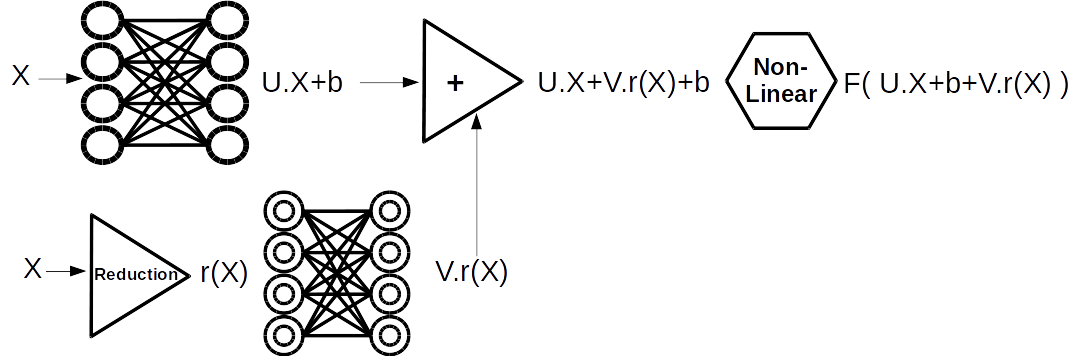
\includegraphics[width=\linewidth]{average_layer}
    \caption{Single layer of the datasetwise neural network. U and V are 2 matrices of the same shape. r(X) is the result of the reduction of the input data X. In practivce the + operator is relying on broadcasting to sum V.r(X) to each sample of X.}
    \label{fig:average_layer}
\end{figure}


\victor{Ecrire + en détails les formules}








\subsection{Sample weights} % (fold)
\label{sub:sample_weights}

\topic{Weighted instances requires weighted reduction functions}

When the studied process includes some very rare events the simulation uses importance sampling. 
The simulation output includes importance weights to allow many rare events to be produced while keeping the distribution of events similar to reality.
The neural network must take into account the importance weights to accurately regress the parameters.
Which leads to use weighted average instead of simple average for example. (and makes maximum and other unweighted reduction ill-suited to this setting)

More precisely, for 2 datasets $D$ and $D^\prime$ if the associated empirical distribution are equal then the neural network output should also be equal.

\begin{equation}
    \forall x, p_D(x) = p_{D^\prime}(x) \implies f(D; \phi) = f(D^\prime; \phi)
\end{equation}

with,
\begin{equation}
    p_D(x) = \sum_{v \in D} w_i \delta (x - v)
\end{equation}
and $\delta$ is the Dirac distribution function.

\begin{figure}[htb]
    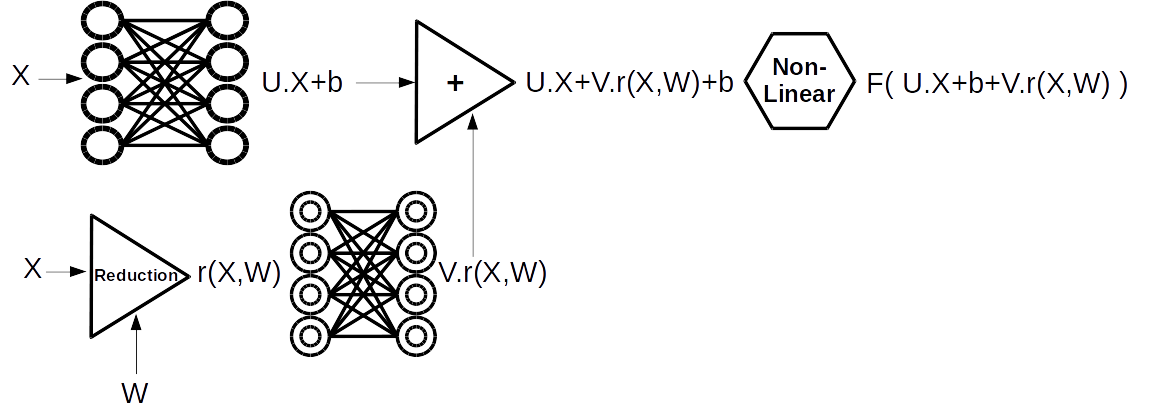
\includegraphics[width=\linewidth]{weighted_average_layer}
    \caption{Single layer of the weighted datasetwise neural network. The reduction function takes into account the sample weights.}
    \label{fig:weighted_average_layer}
\end{figure}


\subsection{Handle nuisance parameter} % (fold)
\label{sub:handle_nuisance_parameter}


\subsubsection{Ignore them} % (fold)
\label{subsub:ignore_them}

\topic{The model can simply learn the marginal posteriors "like a boss"}






\subsubsection{Marginalization} % (fold)
\label{subsub:marginalization}

\topic{Nuisance parameters are marginalized using Monte Carlo integral approximation.}

The objective is to infer the parameter $\mu$ of a model that describes a stochastic system from experimental data $D$.
However $\mu$ alone is not enough to describe the experimental data.
More causal parameters, noted $\alpha$, are required.
Since the parameters $\alpha$ are not the object of study they are tagged as \emph{nuisance} parameters in opposition to the parameter \emph{of interest} $\mu$.

The nuisance parameters have to be marginalized.
\begin{equation}
    p(\mu | x) = \int d\alpha ~ p(\alpha | x) ~ p(\mu | x, \alpha)
\end{equation}

This integral can be approximated with Monte Carlo.

\begin{equation}
  \int d\alpha ~ p(\alpha) ~ f(\alpha)
  \approx \sum_i w_i ~ f(\alpha_i)
\end{equation}

Where $p(\mu | x, \alpha)$ is approximated using a trained MDN as seen previously.
The neural network $f$ produces the mixture parameters $m_i, y_i, \sigma_i$ from the experimental data $x^\star$ and sampled $\alpha$.

\begin{algorithm}[H]
 \For{$i \in [0, N]$}{
  $\alpha_i, w_i$ $\gets$ MC sample from $p(\alpha)$ \;
  $m_j, y_j, \sigma_j = f(x^\star, \alpha; \phi^\star)$ \;
  $\bar\mu = \sum_{j=0}^K m_j y_j $ \;
  $\Delta\mu = \sum_{j=0}^K m_j \left [ \sigma_j^2 + y_j^2 - \bar \mu^2 \right ]$ \;
  $\hat\mu$  $\gets$ $\hat\mu + w_i \times \bar\mu$ \;
  $\hat\sigma$  $\gets$ $\hat\sigma + w_i \times (\bar\mu^2 + \Delta\mu^2)$ \;
 }
$\hat\sigma$  $\gets$ $\hat\sigma - \hat\mu^2$ \;
\caption{Marginalizing the nuisance parameters $\alpha$ using MC to compute the integral.}
\end{algorithm}







\section{Discussing the related work} % (fold)
\label{sec:discussing_the_related_work}



\subsection{INFERNO} % (fold)
\label{sub:inferno}

Using a neural network to directly map the dataset to the estimated parameter distribution can be viewed as an extension of the work done in INFERNO \cite{DECASTRO2019170inferno}. 
Indeed the current state of the art is using a classifier score histogram to produce summary static while INFERNO includes the summary statistic production in the neural network.
In this work the next step, maximum likelihood fit to retrieve the parameter of interest, is also left to the neural network.


\cite{DECASTRO2019170inferno} is the closest work of this study in which the authors optimize a neural network to produce of summary statistics that reduces the uncertainty on the parameters of interest estimation.



\subsection{Neural statistician} % (fold)
\label{sub:neural_statistician}

Neural Statistician \cite{Edwards17neuralstatistician} is also relying on a similar neural network architecture to compute summary statistics.
The idea in Neural Statistician is that similar datasets can be gathered as originating from the same generative model including a global parameter to control the shift between domains.
In this work the architecture is slightly improved to take into account importance weights.
Moreover the objective is completely different since we consider supervised regression.

Causal parameters are often related to properties of the distribution of the data in statistical simulations.
The architecture should reflect this link in order for a neural network to capture the relevant information.
This work is using Mixture density network \cite{Bishop94mixturedensity} combined with neural network architectures design to learn summary statistics on datasets.
Such architecture is shown in \cite{Edwards17neuralstatistician}, in the context of transfer learning and one shot learning, where the neural network is producing summary statistics to embed the link between similar datasets.



\subsection{Others} % (fold)
\label{sub:others}

\victor{Related to Amortized VI ?}
\victor{Related to simple Gaussian fit ?}


\subsection{Limitations} % (fold)
\label{sub:limitations2}


The variance is learned meaning it should be tested as well.
The classic method can measure their variance (from math).
Coverage test ?

Training can be coslty.
The regressor eats datasets, not samples.

 %Domain adaptation
%!TEX root = ../thesis.tex
%*******************************************************************************
%****************************** Fourth Chapter *********************************
%*******************************************************************************

\chapter{Benchmark}
\label{chap:benchmark}
\ifpdf
    \graphicspath{{Chapter4/Figs/Raster/}{Chapter4/Figs/PDF/}{Chapter4/Figs/}}
\else
    \graphicspath{{Chapter4/Figs/Vector/}{Chapter4/Figs/}}
\fi

\topic{Il faut un benchmark solide pour comparer les méthodes}

\section{Constitution du benchmark} % (fold)
\label{sec:constitution_du_benchmark}

\content{Weak baselines, too many (too complex or specific) objective functions and other problems in presenting ML results.}

\victor{Ce que j'essaie de faire c'est mettre un peu d'ordre. Donc je doit décrire les métriques utilisée par les autres papier. Décrire ce que je veux ranger}




\section{Higgs data} % (fold)
\label{sec:higgs_data}




\subsection{Simulation} % (fold)
\label{sub:simulation}

Precise simulation is not only used for training machine learning models.
Simulation is critical for the design of the apparatus itself or planning an upgrade of the apparatus.
Simulation allows to predict how the data should be according to a given version of the standard model.
Theorists updates on the standard model can be validated or rejected efficiently by comparing their predictions through simulation to the data.

Of course simulation of an experiment at the LHC requires tremedous work.
For example the ATLAS simulation \cite{Aad_2010} can be broken down into 3 major steps.
First the event simulation that takes care of the collision, the particles creation, the particle interactions between themselves and their decay to other particles.
Second the interaction between the particles and matter (the apparatus) which is done using Geant4 \cite{AGOSTINELLI2003250}, \cite{1610988}, \cite{ALLISON2016186}.
This is the part I find the most impressive.
Sensors, magnetic field generated by the electronics, cables, even the air or the cooling liquids are taken into account.
Finally digitization deals with what numbers will come out of the previous interaction to be finally stored for later analysis.
Although very accurate simulations of all parts and phenomena is technically possible the computation power often limits its usage to more approximative ones. 
This leads to creating a custom tradeoff for each analysis to focus computation on the most relevant parts.

Interaction between particles and the sensors are again fundamentally stochastic.
A very large number of sensors is required to reach a high enough resolution to make accurate measurements.
As a consequence each sensor interaction with a particle creates a latent variable in the modeling of a single event.
Therefore 100 000 detector pieces lead to 100 000 latent variables making the marginal likelihood intractable (see \autoref{sub:inverse_problem}).

Simulation is expensive and possible processes include very rare events like Higgs boson creation.
Without \emph{importance sampling}\needcite it would be impossible to simulate enough events to get a representative sample of those rare processes.
Simulation runs independently for every processes.
Then the data are gathered with importance weights reprensenting their relative probability of occurrence.





\subsection{HiggsML challenge} % (fold)
\label{sub:higgsml_challenge}


The data were initially produced for the HiggsML challenge \cite{Adam-Bourdarios2014}.
It was a the most successfull challenge of its time with (some number of teams and submissions).
The data is now publicly available \needcite.
\victor{TODO : citer les autres articles qui ont utilisés HiggsML}

The HiggsML dataset is composed of 818238 events described by 17 primary features and 13 features derived from the primaries.
Near the end of the challenge X more constructed features known as "cooked features" became popular \needcite.
The cooked features help getting good classification perfomances\needcite in some context (what context ?).
The label designing if the event is a signal ($H\to \tau \tau$) or a backgroud (any other process) is of course available in the dataset as well.

Sample weights used for the kaggle challenge is not the same ... why again ?




\subsection{Fast re-simulator} % (fold)
\label{sub:fast_re_simulator}


In order to ease experiments, the first part of this work is to build a fast re-simulator of the events.
Indeed one event require on min of CPU time to be generated.
Regenerating the entire dataset for all the set of parameters values we might want to try would be too expensive.
However the parameters considered in this work only affect some of the final parts of the simulation and can be computed a posteriori.

A small library was published\needcite and a more recent version is available here\needcite.
This rest of this section will briefly explain how the event are re-generated for a different set of parameters.

The parameter of interest $\mu$ is the deviation of the expected number of signal from the predictions of the standard model.
Recomputing the data only requires to multiply the sample weights of the signal events with $\mu$.
This is already enough to build a complete workflow of the inference without nuisance parameter.

5 nuisance parameters are considered : tau energy scale, lepton energy scale, jet energy scale, soft term, nasty backgrounds.

\subsubsection{Energy scales} % (fold)
\label{ssub:energy_scales}

The tau energy scale is comming from apparatus imperfections leading to a slightly wrong scale of the measured energy of tau particle.
The lepton and jet energy scale are exactly analogus but with lepton particle and jets.
The 3 energy scales are independant from each other leading to 3 nuisance parameters $\alpha_{tes}, \alpha_{les}, \alpha_{jes}$. 
This nuisance parameter is basically a proportional factor on one or several primary features (eg. PRI\_tau\_pt) stained with non negligeable uncertainty.
Recomputing the events for a different value of the energy scale requires not only to multiply the primary features with the updated value but also all the features derived from this primaries.

\subsubsection{Soft term} % (fold)
\label{ssub:soft_term}

The missing energy transverse (met) is perturbated by a random vector sampled from a normal distribution which standard deviation is our nuisance parameter $\alpha_{st}$.
This is a more difficult systematic effect to infer from the data.
Just like the parameter of interest it isby definition impossible to infer the soft term from one example.


\subsubsection{Nasty background} % (fold)
\label{ssub:nasty_background}

The background distribution is a mixture of several processes.
The mixture coefficient of one of these processes is not known with enough precision.
\victor{c'est celui avec un detailLabel = W}
This nuisance parameter $\alpha_{nb}$ only requires to recompute the weights.
Since the parameter of interest is also linked with the sample weights, ie the amount of events, this nuisance parameter directly leads to an increase of the variance of our estimator $\hmu$.
Indeed a larger number of events in a bin can now be explained by an increase of $\mu$ or an increase of $\alpha_{nb}$.



\subsubsection{Mass MMC} % (fold)
\label{ssub:mass_mmc}

Unfortunately the MMC mass (what the hell is it ?) cannot be easilly recomputed from primaries.
Computing the MMC mass involves an expensive optimization step \victor{More details ?}.
Although DER\_Mass\_MMC is the a relevant feature (\textbf{see missing figure}) for classification it is removed from the dataset.

\victor{TODO : figure top 5 or top 10 feature importances}




\subsubsection{Bootstraping} % (fold)
\label{ssub:boostraping}


Re-generating the data is not the same as re-running the simulation.
\victor{Results on boostrapping that says when it is OK to do it ?}

Training the direct regression method requires way more data than training a classifier since a sample for a regressor is composed of thousands of events.
With boostrapping and considering the re-generation as data augmentation the finite HiggsML dataset can be turned into an almost infinite generator of events.




\section{Toy datasets} % (fold)
\label{sec:toy_datasets}


Toy datasets allow a full control of the generative process and the properties of the data.
It is a necessary step to produce a test bed of the program code.
But also to evaluate the influence of many parameter (eg. number of dimension, number of sample, signal/background separability, etc) on the performances to help explain the performances on real data.






\subsection{Toy 1D} % (fold)
\label{sub:toy_1d}

The first toy is a very simple case of estimation of a mixture coefficient in the presence of one systematic effect.
The likelihood is known and tracktable making maximum likelihood and bayesian inference possible.
Comparing the inference methods to the best possible inference is a first step to validate them.


The toy generative process is a mixture of 2 distributions with one observable $x \in \RR$.
The background distribution is a gamma distribution versus a gaussian distribution for the signal process.
\autoref{fig:minitoy_distrib} presents the data distribution.
To make the problem non trivial and correspond more to reality the signal distribution is overlapping with the background distribution.

The parameter of interest is the mixing coefficient $\mu$ of the 2 distributions.
The nuisance parameter $\alpha$ is a rescaling of the observable $x$.

Without nuisance parameter $\alpha$ the likelihood is :
$$
    p(x | \mu) = \mu \mathcal N(x|a, d) + (1-\mu) \Gamma(x|k, l)
$$

with $N(x|a, d)$ a gaussian with mean $a$ and standard deviation $d$ and $\Gamma(x|k, l)$ a gamma distribution with $k$ ... and $l$ the localization  ... ????
The chosen values are : $a = 5, d=0.5, k=2, l=0$.


Including nuisance parameter $\alpha$ the likelihood becomes :
$$
    p(x | \mu, \alpha) = \mu \mathcal N(x|\alpha a, \alpha d) + (1-\mu) \Gamma(x|\alpha k, l)
$$

\begin{figure}[htb]
    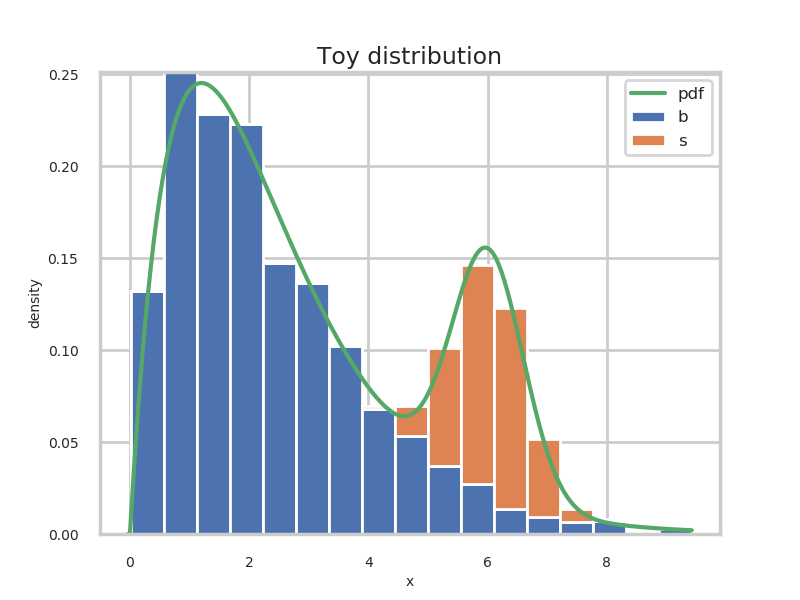
\includegraphics[width=\linewidth]{minitoy/distrib.png}
    \caption{Data distribution of the 1D toy for a 10,000 instances sampling}
    \label{fig:minitoy_distrib}
\end{figure}






\subsection{Toy 3D} % (fold)
\label{sub:toy_3d}

To get closer to reality the toy example introduced in \cite{DECASTRO2019170inferno} is also included.
It is a mixture of 2 processes : $f_b$ for the backgrounds and $f_s$ for the signals.

\begin{equation}
	f_b (x|r, \lambda) = \mathcal N \left ( (x_0, x_1) | (2+r, 0) 
	\begin{bmatrix} 5 & 0 \\ 0 & 9 \end{bmatrix} \right ) Exp((x_2| \lambda)
\end{equation}
\begin{equation}
	f_s (x|r, \lambda) = \mathcal N \left ( (x_0, x_1) | (1, 1) 
	\begin{bmatrix} 1 & 0 \\ 0 & 1 \end{bmatrix} \right ) Exp((x_2| 2)
\end{equation}

Leading to the likelihood :
\begin{equation}
	p(x | r, \lambda, \mu ) = (1-\mu) f_b(x|r, \lambda) + \mu f_s(x|r, \lambda)
\end{equation}

This toy is multi dimensional, more complex and includes 2 nuisance parameters.
The nuisance parameters affects only the background distribution.
Once again the background and signal distribution are overlapping.
\autoref{fig:s3d2_pairgrid} shows the distributions of a sampled dataset.

\begin{figure}[htb]
    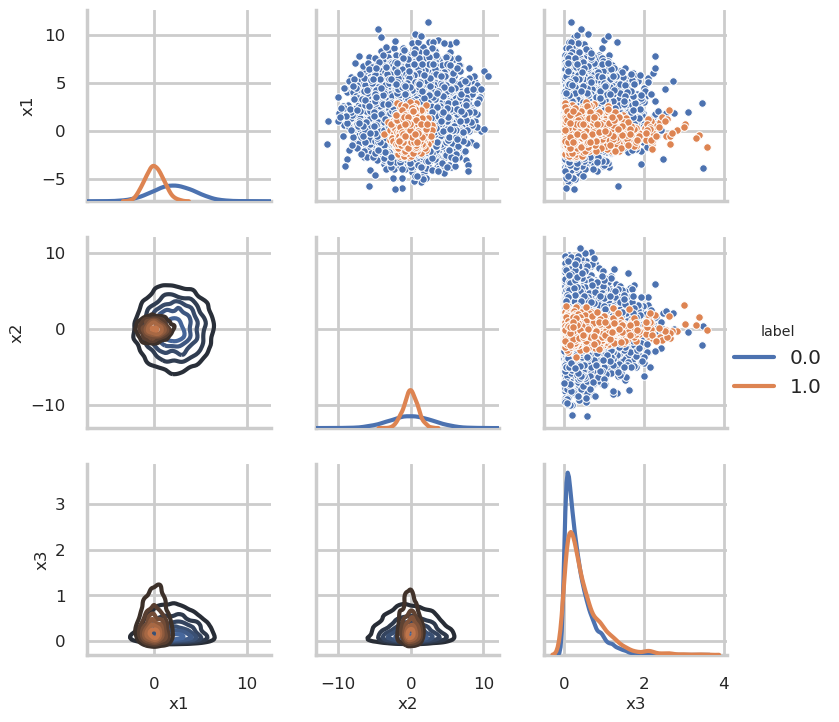
\includegraphics[width=\linewidth]{s3d2/pairgrid}
    \caption{Data distribution of the 3D toy}
    \label{fig:s3d2_pairgrid}
\end{figure}






\section{Bayesian inference on toys} % (fold)
\label{sec:bayesian_inference_on_toys}


The toy problems (see \autoref{sub:toy_1d} and \autoref{sub:toy_3d} ) do not suffer from intractable likelihood making it possible to compute the posterior probability using standard bayesian inference.
The computed posterior is the best possible inference and will be compared with the other methods that assumes the samplewise likelihood is intractable.

\subsection{Computing the posterior} % (fold)
\label{sub:computing_the_posterior}

The posterior probability density function of the parameter of interest $p(\mu|D)$ can be computed from the likelihood and a prior.
The prior is chosen as uniform over the domain of possible values of $\mu$.

From Bayes theorem : 
\begin{equation}
    p(\mu, \alpha | D) = \frac{p(D|\mu, \alpha) p(\mu, \alpha)}{p(D)}
\end{equation}
and
\begin{equation}
	p(\mu|D) = \int_{\alpha} p(\mu, \alpha | D) p(\alpha|D) d\alpha
\end{equation}



Computing the integral by hand can be tedious.
The simple method proposed allow to avoid it.

Start with a grid, fine enough, going through the possible values. $\mu_i, \alpha_j$.
\begin{equation}
    p(\mu_i, \alpha_j | x) = \frac{p(x|\mu_i, \alpha_j) p(\mu_i, \alpha_j)}{p(x)}
\end{equation}


The 2 following tensor can be computed from the simulator.
\begin{itemize}
  \item likelihood : $L_{ij} = p(x|\mu_i, \alpha_j)$
  \item prior : $K_{ij} = p(\mu_i, \alpha_j)$ 
\end{itemize}

giving the tensor $ R_{ij} = p(x|\mu_i, \alpha_j) p(\mu_i, \alpha_j) $ 
which after renormalization gives the posterior tensor $ T_{ij} = p(\mu_i, \alpha_j | x)$.

The marginal probabilities are computed from $T_{ij}$ :
\begin{itemize}
  \item $p(\mu_i | x) = \sum_j T_{ij} = Y_i$
  \item $p(\alpha_j | x) = \sum_i T_{ij} = A_j$
\end{itemize}

the neural network should compute : $p(\mu_i | x, \alpha_j) = \frac{p(\mu_i, \alpha_j | x)}{p(\alpha_j | x)} = \frac{T_{ij}}{A_j} = N_{ij}$

We then obtain the quantities we are interested in :
\begin{itemize}
  \item $ \VV(\mu|x) = \VV(\mu_i, Y_i) $
  \item $ \EE_{\alpha \sim p(\alpha|x)}[ \VV(\mu|x, \alpha) ] = \sum_j \VV(\mu|x, \alpha_j) p(\alpha_j | x) = \sum_j \VV_i(\mu_i, N_{ij}) A_j$
  \item $\EE_{\alpha \sim p(\alpha|x)} \left ((\EE [\mu|x, \alpha]  - \EE[\mu|x])^2\right ) = \VV(\mu|x) - \EE_{\alpha \sim p(\alpha|x)}[ \VV(\mu|x, \alpha) ] = \VV(\mu_i, Y_i) - \sum_j \VV_i(\mu_i, T_{ij}) A_j$
\end{itemize}


\subsubsection{Note 1}

For the computations it is necessary to remember that the tensors contain probabilities !
Meaning $<\mu|x>= \EE[\mu|x] = \sum_i y_i Y_i$ because $Y_i$ only contains probability densities, not values of $y$ !

Same applies for $\VV(\mu|x) = \sum_i \mu_i^2 Y_i - <\mu|x>^2 = \VV(\mu_i, Y_i)$


\subsubsection{Note 2}

For numerical stability it is best to work with log probabilities.

Indeed $x$ is a dataset so $p(x | \mu_i, \alpha_j) = \prod_k^N p(x_k | \mu_i, \alpha_j)$ for N big enough to obtain too small number to be stored in 64 bits.

It is smarter to compute : $\log p(x | \mu_i, \alpha_j) = \sum_k^N log p(x_k | \mu_i, \alpha_j) = \ell(x | \mu_i, \alpha_j)$
Then $\ell(\mu_i, \alpha_j| x) = \log p(x|\mu_i, \alpha_j) + \log p(\mu_i, \alpha_j)$

And renormalizing using a softmax :
$$ 
    T_{ij} = p(\mu_i, \alpha_j | x) = \frac{e^{\ell(\mu_i, \alpha_j| x)} }{\sum_{n,m} e^{\ell(\mu_n, \alpha_m| x)} }
$$


\subsubsection{Note 3}

If there is multiple nuisance parameters $\alpha$, $\beta$, etc the tensor are simply n-dimensional : $L_{ijk...}$, $T_{ijk...}$, $K_{ijk...}$, etc.
And all sums over $j$ become summs over $j,k, ...$ which is easily handle with broadcasting in modern numeric libraries.



\section{Evaluation metric} % (fold)
\label{sec:evaluation_metric}

\topic{The evaluation metric is the empirical mean squared error on the estimated parameters including variances}

Many methods to estimate the parameter of interest and its variance are available.
If changing the set of hyper parameter for the learning procedure is considered as changing the method then countless methods are to be evaluated.
Automating the measure of the performances of a proposed method is crucial to select the best method.
In this section is described a simple but general procedure to measure the performances of a given method.

The usual criterions to evaluate an estimator $\htheta$ are the bias, the variance and the mean squared error defined as follow :
\begin{equation}
  Bias(\htheta) = \EE[\htheta] - \thetas
\end{equation}
\begin{equation}
  Var(\htheta) = \EE[ (\htheta - \EE[\htheta])^2 ] = \EE[\htheta^2] - (\EE[\htheta])^2
\end{equation}
\begin{equation}
  MSE(\htheta) = \EE[(\htheta - \thetas)^2] = Var(\htheta) + [Bias(\htheta)]^2
\end{equation}

To evaluate these criterion we need to repeat the experiement $N$ times leading to many estimation of the parameters $\hmu^{(k)}$ and $\hshmu^{(k)}$.
Repeating the experiment can be done through cross-validation methods.


\subsection{Evaluation of the parameter of interest estimator} % (fold)
\label{sub:evaluation_of_the_parameter_of_interest_estimator}

First, let's focus on evaluating the estimator of the parameter of insterest $\hmu$.
The true value of $\mu$, noted $\mus$, is available during tests since it is an input of the simulator.

From the estimation of its expected value
\begin{equation}
  \EE[\hmu] \approx <\hmu^{(k)}>_k = \frac{1}{N} \sum_{k} \hmu^{(k)}
\end{equation}
it is possible to estimated the criterions

\begin{equation}
  Bias(\hmu) \approx <\hmu^{(k)}>_k - \mus
\end{equation}
\begin{equation}
  \label{eq:var_hmu}
  Var(\hmu) \approx <\hmu^{(k)} \times \hmu^{(k)}>_k - (<\hmu^{(k)}>_k)^2
\end{equation}
\begin{equation}
  MSE(\hmu) = Var(\hmu) + [Bias(\hmu)]^2
\end{equation}




\subsection{Evaluation of the variance estimator} % (fold)
\label{sub:evaluation_of_the_variance_estimator}

The evaluation of the variance estimator $\hshmu$ could be done in the same way if the true variance $Var(\hmu)$ can be computed.
If this is not the case an approximation is available using \autoref{eq:var_hmu}.

\begin{equation}
  Bias(\hshmu) \approx <\hshmu^{(k)}>_k - Var(\hmu)
\end{equation}
\begin{equation}
  Var(\hshmu) \approx <\hshmu^{(k)} \times \hshmu^{(k)}>_k - (<\hshmu^{(k)}>_k)^2
\end{equation}
\begin{equation}
  MSE(\hshmu) = Var(\hshmu) + [Bias(\hshmu)]^2
\end{equation}


 %New methods : INFERNO, Mining gold, etc
%!TEX root = ../thesis.tex
%*******************************************************************************
%******************************  5th  Chapter **********************************
%*******************************************************************************

\chapter{Experimental results}
\label{chap:xp}
% **************************** Define Graphics Path **************************
\ifpdf
    \graphicspath{{Chapter5/Figs/Raster/}{Chapter5/Figs/PDF/}{Chapter5/Figs/}}
\else
    \graphicspath{{Chapter5/Figs/Vector/}{Chapter5/Figs/}}
\fi




\section{Technical difficulties} % (fold)
\label{sec:technical_difficulties}

Where do I write about the numerous issues ?
\begin{itemize}
  \item Inferno is unstable
  \item Pivot is unstable
  \item TP requires Jacobian vector product or takes crazy amount of time to train
  \item Regressor requires slow Adam and is probably a pain to train with gaussian mixture
  \item 
\end{itemize}



The benchmark is controlled with many parameters
\begin{itemize}
  \item Number of test samples
  \item Parameter of the toy model
  \item True value of the parameter of interest and nuisance parameters
  \item Sampling random seed
  \item TODO finish this list
\end{itemize}








\section{Performances on toys} % (fold)
\label{sec:performances_on_toys}

The idea is to do one subsection for one result 
\begin{itemize}
  \item Result 1 : The more test samples the better the inference
  \item Result 2 : Calib > Prior as expected
  \item Result final : Who is the best ? 
  \item 5. Regressor estimated variance is probably broken
\end{itemize}


Let's start with the results on the two toy problems (see \autoref{sec:toy_datasets} for details).
Toys provides a fully controled environement on various parameters of the problem to confront the proposed methods against different difficulties.
The first one is the small number of samples to do inference (\autoref{sub:performance_according_to_sample_size}).










\subsection{Performance according to sample size} % (fold)
\label{sub:performance_according_to_sample_size}

Here is summaried the performances measured according to the number of sample of the test set.

On the nominal test set (\autoref{fig:gg_baseline_nominal_n_samples_mse}) the MSE behave as expected \ie decreases fast ($\frac{1}{\sqrt{N}}$) as the size of the test set increase.
Only direct regression seems to not depend on the test size.
This is unexpected and cannot only be explained by the fact that the neural network is trained with fixed dataset size and did not learn to improve as the test set size increase...



\begin{figure}[ht!]
  \centering
  \begin{subfigure}[t]{0.49\linewidth}
    \includegraphics[width=\linewidth]{COMPARE/GG-prior/GradientBoostingModel/profusion_nominal_n_samples_mse.png}
    \caption{Gradient boosting}
    % \label{fig:gg-prior_GB_profusion_nominal_n_samples_mse}
  \end{subfigure}%
  \hfill
  \begin{subfigure}[t]{0.49\linewidth}
    \includegraphics[width=\linewidth]{COMPARE/GG-prior/NeuralNetClassifier/profusion_nominal_n_samples_mse.png}
    \caption{Neural network classifier}
    % \label{fig:gg-calib_best_average_errplot_mse}
  \end{subfigure}

  \begin{subfigure}[t]{0.49\linewidth}
    \includegraphics[width=\linewidth]{COMPARE/GG-prior/DataAugmentation/profusion_nominal_n_samples_mse.png}
    \caption{Data augmentation}
    % \label{fig:gg-prior_GB_profusion_nominal_n_samples_mse}
  \end{subfigure}%
  \hfill
  \begin{subfigure}[t]{0.49\linewidth}
    \includegraphics[width=\linewidth]{COMPARE/GG-prior/TangentPropClassifier/profusion_nominal_n_samples_mse.png}
    \caption{Tangent Prop}
    % \label{fig:gg-calib_best_average_errplot_mse}
  \end{subfigure}

  \begin{subfigure}[t]{0.49\linewidth}
    \includegraphics[width=\linewidth]{COMPARE/GG-prior/Inferno/profusion_nominal_n_samples_mse.png}
    \caption{Inferno}
    % \label{fig:gg-prior_GB_profusion_nominal_n_samples_mse}
  \end{subfigure}%
  \hfill
  \begin{subfigure}[t]{0.49\linewidth}
    \includegraphics[width=\linewidth]{COMPARE/GG-prior/PivotClassifier/profusion_nominal_n_samples_mse.png}
    \caption{Pivot classifier}
    % \label{fig:gg-calib_best_average_errplot_mse}
  \end{subfigure}

  \begin{subfigure}[t]{0.49\linewidth}
    \includegraphics[width=\linewidth]{COMPARE/GG-prior/Regressor/profusion_nominal_n_samples_mse.png}
    \caption{Regressor}
    % \label{fig:gg-prior_GB_profusion_nominal_n_samples_mse}
  \end{subfigure}%
  \hfill
  \begin{subfigure}[t]{0.49\linewidth}
    \includegraphics[width=\linewidth]{COMPARE/GG-marginal/Regressor/profusion_nominal_n_samples_mse.png}
    \caption{Regressor marginal}
    % \label{fig:gg-calib_best_average_errplot_mse}
  \end{subfigure}


  \caption{MSE of $\hmu$ according to the number of samples on nominal data only. Each curve correspond to a model with a specific set of hyper-parameter.}
  \label{fig:gg_baseline_nominal_n_samples_mse}
\end{figure}


This is less obvious on the calibrated data where increasing the number of samples does not help that much (\autoref{fig:gg_baseline_n_samples_mse}).

The 1D toy problem (named GG) is asymetric in $\alpha$.
Indeed increasing $\alpha$ will move appart the center of the signal and the background distribution.
Also when comparing the nominal distribution and the one with a decreased $\alpha$ with a small amount on signal the signal spike could be confused with a flucuation making inference harder.
This is why blue curves $\alpha=0.8$ are way above the $\alpha=1.2$ curves in most models.

Inferno and the marginal Regressor are not affected by this assymetry.
Maybe those 2 neural networks are measuring $\alpha$ then correcting it ?
The marginal Regressor is expected to do so at least.

\victor{TODO : Wait for new Pivot runs to comment on it.}


\begin{figure}[ht!]
  \centering
  \begin{subfigure}[t]{0.49\linewidth}
    \includegraphics[width=\linewidth]{COMPARE/GG-prior/GradientBoostingModel/profusion_n_samples_mse.png}
    \caption{Gradient boosting}
    % \label{fig:gg-prior_GB_profusion_n_samples_mse}
  \end{subfigure}%
  \hfill
  \begin{subfigure}[t]{0.49\linewidth}
    \includegraphics[width=\linewidth]{COMPARE/GG-prior/NeuralNetClassifier/profusion_n_samples_mse.png}
    \caption{Neural network classifier}
    % \label{fig:gg-calib_best_average_errplot_mse}
  \end{subfigure}

  \begin{subfigure}[t]{0.49\linewidth}
    \includegraphics[width=\linewidth]{COMPARE/GG-prior/DataAugmentation/profusion_n_samples_mse.png}
    \caption{Data augmentation}
    % \label{fig:gg-prior_GB_profusion_n_samples_mse}
  \end{subfigure}%
  \hfill
  \begin{subfigure}[t]{0.49\linewidth}
    \includegraphics[width=\linewidth]{COMPARE/GG-prior/TangentPropClassifier/profusion_n_samples_mse.png}
    \caption{Tangent Prop}
    % \label{fig:gg-calib_best_average_errplot_mse}
  \end{subfigure}

  \begin{subfigure}[t]{0.49\linewidth}
    \includegraphics[width=\linewidth]{COMPARE/GG-prior/Inferno/profusion_n_samples_mse.png}
    \caption{Inferno}
    % \label{fig:gg-prior_GB_profusion_n_samples_mse}
  \end{subfigure}%
  \hfill
  \begin{subfigure}[t]{0.49\linewidth}
    \includegraphics[width=\linewidth]{COMPARE/GG-prior/PivotClassifier/profusion_n_samples_mse.png}
    \caption{Pivot classifier}
    % \label{fig:gg-calib_best_average_errplot_mse}
  \end{subfigure}

  \begin{subfigure}[t]{0.49\linewidth}
    \includegraphics[width=\linewidth]{COMPARE/GG-prior/Regressor/profusion_n_samples_mse.png}
    \caption{Regressor}
    % \label{fig:gg-prior_GB_profusion_n_samples_mse}
  \end{subfigure}%
  \hfill
  \begin{subfigure}[t]{0.49\linewidth}
    \includegraphics[width=\linewidth]{COMPARE/GG-marginal/Regressor/profusion_n_samples_mse.png}
    \caption{Regressor marginal}
    % \label{fig:gg-calib_best_average_errplot_mse}
  \end{subfigure}

  \caption{MSE of $\hmu$ according to the number of samples. Each curve correspond to a model with a specific set of hyper-parameter and a value of $\alpha^\star$. The colors correspond to the values of $\alpha^\star$. Here only the value of $\mu^\star$ is kept as nominal.}
  \label{fig:gg_baseline_n_samples_mse}
\end{figure}



\victor{Evolution de la variance stat et syst en fonction de N\_samples.}







\subsection{Calibration influence} % (fold)
\label{sub:calibration_influence}


In this benchmark two way of calibrating the data is used.
\begin{enumerate}
  \item Trust a given prior
  \item Infer the nuisance parameter distribution using a regressor
\end{enumerate}

Here we show that the later is a better choice and improves significantly the performances of all methods.
Indeed using only a poorly informed prior leads the baseline to a biased estimator.
\autoref{fig:gg_baseline_compare_calib_estimator} shows the estimation of a neural net classifier.
It is clear that the estimation depends on $\alpha^\star$ and is biased if $\alpha^\star$ is not the nominal value.
\victor{TODO : GB \& TP \& REG show the same behaviour. INFERNO is not affected. DA is more robust. Waiting for PIVOT results}

Using the given data to improve calibration leads to an unbiased estimator.
\victor{TODO : Someone may argue that it is because my prior calibration is bad. But my simulator cannot do better...}



\begin{figure}[ht!]
  \centering
  \begin{subfigure}[t]{0.49\linewidth}
    \includegraphics[width=\linewidth]{COMPARE/GG-prior/NeuralNetClassifier/profusion_true_mu_target_mean.png}
    \caption{Prior calibration}
    % \label{fig:gg-prior_GB_profusion_n_samples_mse}
  \end{subfigure}%
  \hfill
  \begin{subfigure}[t]{0.49\linewidth}
    \includegraphics[width=\linewidth]{COMPARE/GG-calib/NeuralNetClassifier/profusion_true_mu_target_mean.png}
    \caption{Using data in calibration to infer $\alpha$}
    % \label{fig:gg-calib_best_average_errplot_mse}
  \end{subfigure}
  \caption{Many estimations of neural net classifier. Each point is colored according to the value of $\alpha^\star$. The x-axis is representing the value of $\mu^\star$. Each point is the average of the estimated interest parameter ($\hmu$) over cross validation of one neural network classifier (one hyper-parameter set).}
  \label{fig:gg_baseline_compare_calib_estimator}
\end{figure}


The 1D toy problem is asymetric by definition which leads to an asymetry in performances when using the prior calibration.
This asymetry tends to disapear when the calibration is done on the data (see \autoref{fig:gg_baseline_compare_calib_n_samples_mse}).


\begin{figure}[ht!]
  \centering
  \begin{subfigure}[t]{0.49\linewidth}
    \includegraphics[width=\linewidth]{COMPARE/GG-prior/NeuralNetClassifier/profusion_n_samples_mse.png}
    \caption{Prior calibration}
    % \label{fig:gg-prior_GB_profusion_nominal_n_samples_mse}
  \end{subfigure}%
  \hfill
  \begin{subfigure}[t]{0.49\linewidth}
    \includegraphics[width=\linewidth]{COMPARE/GG-calib/NeuralNetClassifier/profusion_n_samples_mse.png}
    \caption{Using data in calibration to infer $\alpha$}
    % \label{fig:gg-calib_best_average_errplot_mse}
  \end{subfigure}
  \caption{Calibration is the main influence on the inference.}
  \label{fig:gg_baseline_compare_calib_n_samples_mse}
\end{figure}









\subsection{Compare methods} % (fold)
\label{sub:compare_methods}


The good news is that systematic aware learning and the direct approach is giving better results that the baseline (\autoref{fig:compare_gg_best_mse}).

\begin{figure}[ht!]
  \centering
  \begin{subfigure}[t]{0.49\linewidth}
    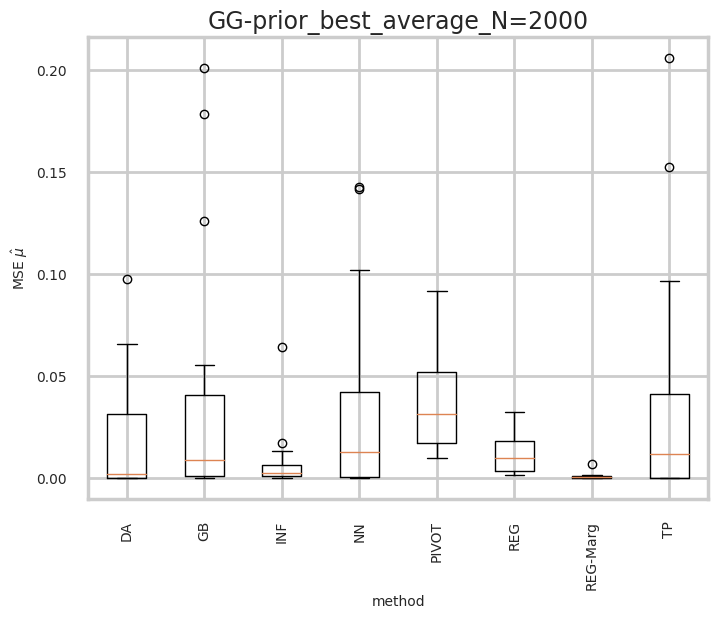
\includegraphics[width=\linewidth]{COMPARE/GG-prior/BEST_MSE/GG-prior_best_average_N=2000-boxplot_mse.png}
    \caption{Boxplot of MSE on Prior}
    % \label{fig:gg-prior_best_average_boxplot_mse}
  \end{subfigure}%
  \hfill
  \begin{subfigure}[t]{0.49\linewidth}
    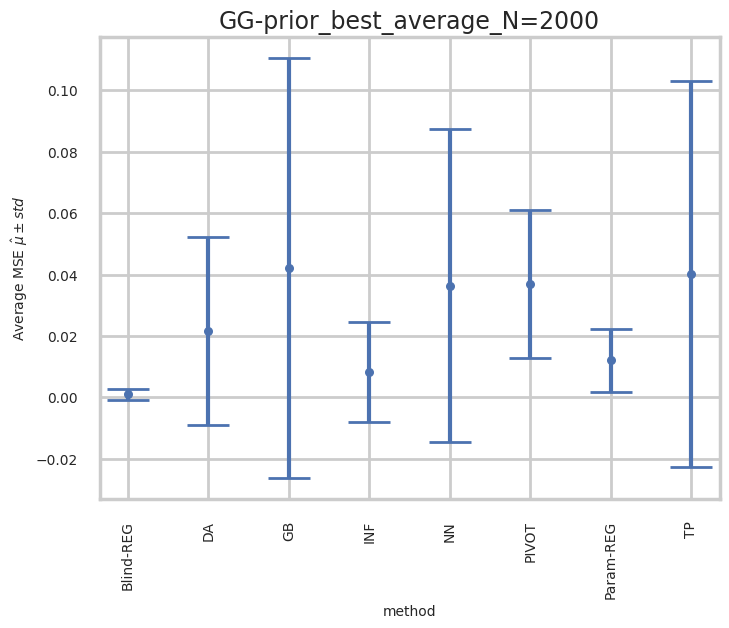
\includegraphics[width=\linewidth]{COMPARE/GG-prior/BEST_MSE/GG-prior_best_average_N=2000-errplot_mse.png}
    \caption{Average MSE $\pm$ variance on Prior}
    % \label{fig:gg-prior_best_average_errplot_mse}
  \end{subfigure}

  \begin{subfigure}[t]{0.49\linewidth}
    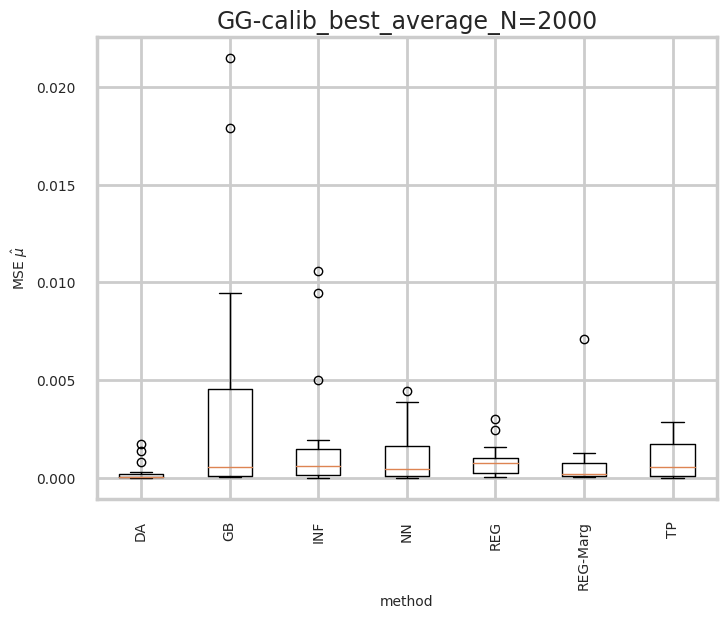
\includegraphics[width=\linewidth]{COMPARE/GG-calib/BEST_MSE/GG-calib_best_average_N=2000-boxplot_mse.png}
    \caption{Boxplot of MSE on Calibrated GG}
    % \label{fig:gg-prior_best_average_boxplot_mse}
  \end{subfigure}%
  \hfill
  \begin{subfigure}[t]{0.49\linewidth}
    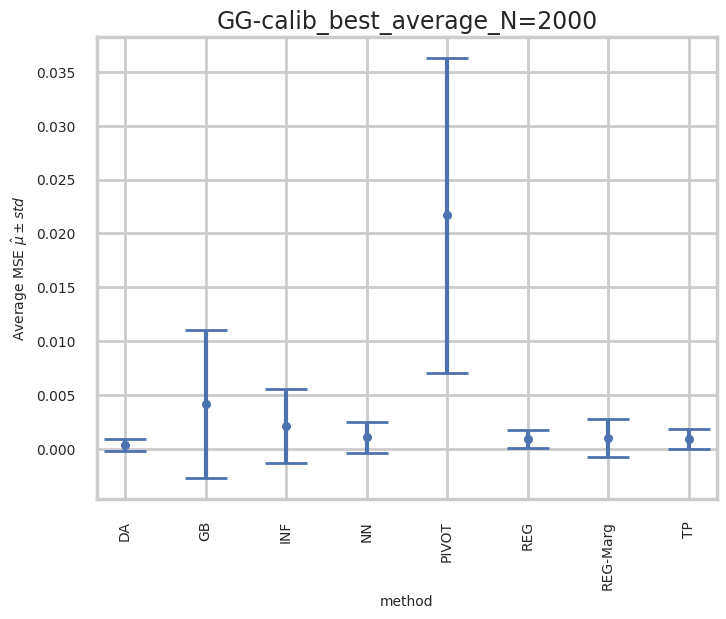
\includegraphics[width=\linewidth]{COMPARE/GG-calib/BEST_MSE/GG-calib_best_average_N=2000-errplot_mse.png}
    \caption{Average MSE $\pm$ variance on Calibrated GG}
    % \label{fig:gg-calib_best_average_errplot_mse}
  \end{subfigure}

  \caption{Best MSE on GG with 2000 test samples. Distribution according to $\mu^\star$ and $\alpha^\star$.}
  \label{fig:compare_gg_best_mse}
\end{figure}

Reg-Marginal is very good on the 1D toy problem which may be explained by the simplicity of the problem.
The average of the only observable $x$ is linearly connected to the parameter of interest (see \autoref{fig:gg_mean_link}).
The only extra work the marginal regressor has to do is to infer $\alpha$ to adjust itsinference which is also very simple in this toy.

\begin{figure}[ht!]
  \centering
  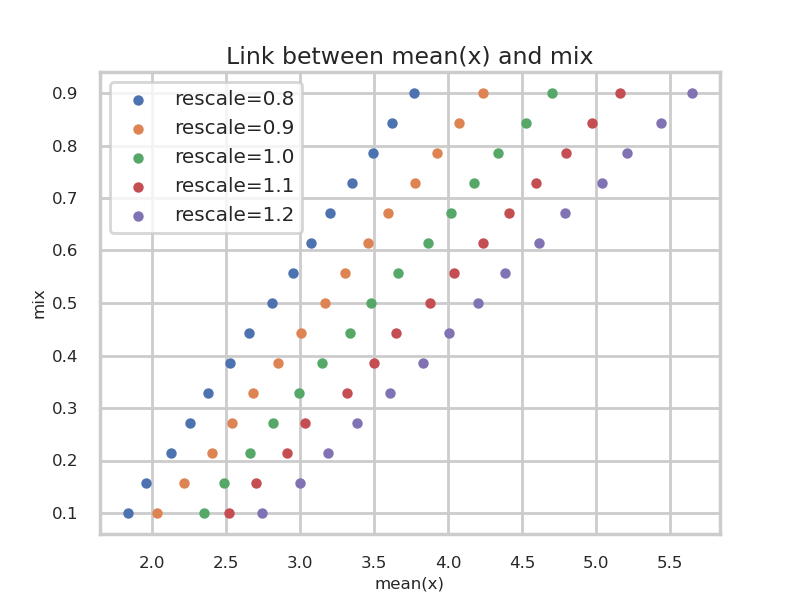
\includegraphics[width=0.49\linewidth]{GG/mean_link.png}
  \caption{link between $\mu^\star$ and the average of $x$ on GG toy problem}
  \label{fig:gg_mean_link}
\end{figure}


Inferno is doing very well including on the Prior calibration.

Tangent propagation is failing to learn a robust distribution.
This is expected as the only feature $x$ is both very correlated to the parameter of interest but also to the nuisance parameter.
Making the classification good and independant from $\alpha$ at the sample level is not possible.

Data augmentation is very good !
Data augmentation is learning to be less confident about the classification which spread the score distribution of the signals.
This spreading leads to splitting signal events into 2 bins instead on one (see \autoref{fig:gg_prior_distrib_summaries}).
\textbf{But how is it helping inference ???}

\begin{figure}[ht!]
  \centering
  \begin{subfigure}[t]{0.49\linewidth}
    \includegraphics[width=\linewidth]{GG-prior/NN/valid_distrib.png}
    \caption{NN score distribution}
    % \label{fig:gg-prior_best_average_boxplot_mse}
  \end{subfigure}%
  \hfill
  \begin{subfigure}[t]{0.49\linewidth}
    \includegraphics[width=\linewidth]{GG-prior/DA/valid_distrib.png}
    \caption{DA score distribution}
    % \label{fig:gg-prior_best_average_errplot_mse}
  \end{subfigure}

  \begin{subfigure}[t]{0.49\linewidth}
    \includegraphics[width=\linewidth]{GG-prior/NN/valid_summaries.png}
    \caption{NN summaries}
    % \label{fig:gg-prior_best_average_boxplot_mse}
  \end{subfigure}%
  \hfill
  \begin{subfigure}[t]{0.49\linewidth}
    \includegraphics[width=\linewidth]{GG-prior/DA/valid_summaries.png}
    \caption{DA summaries}
    % \label{fig:gg-calib_best_average_errplot_mse}
  \end{subfigure}

  \caption{Score distribution and bin counts for NN classifier and data augmentation}
  \label{fig:gg_prior_distrib_summaries}
\end{figure}



\victor{TODO : Compare methods also according to number of samples ! REG and DA are very good with small test size}
The regressor and data augmentation are very good with small test size \autoref{fig:compare_gg_best_mse50_samples} even when using only prior calibration.

\begin{figure}[ht!]
  \centering
  \begin{subfigure}[t]{0.49\linewidth}
    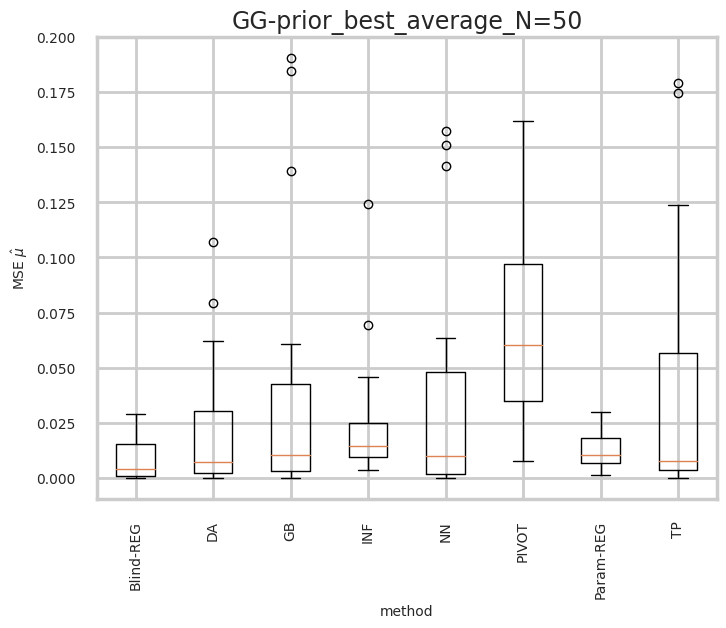
\includegraphics[width=\linewidth]{COMPARE/GG-prior/BEST_MSE/GG-prior_best_average_N=50-boxplot_mse.png}
    \caption{Boxplot of MSE on Prior}
    % \label{fig:gg-prior_best_average_boxplot_mse}
  \end{subfigure}%
  \hfill
  \begin{subfigure}[t]{0.49\linewidth}
    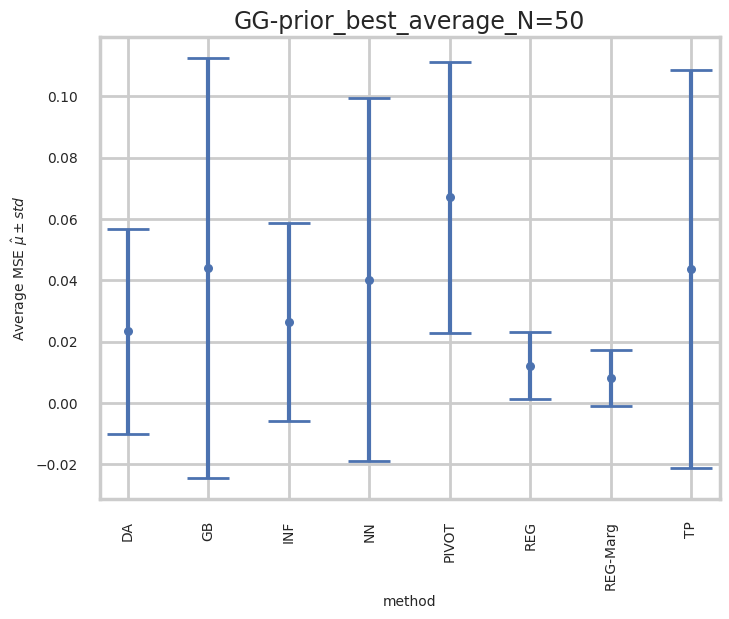
\includegraphics[width=\linewidth]{COMPARE/GG-prior/BEST_MSE/GG-prior_best_average_N=50-errplot_mse.png}
    \caption{Average MSE $\pm$ variance on Prior}
    % \label{fig:gg-prior_best_average_errplot_mse}
  \end{subfigure}

  \begin{subfigure}[t]{0.49\linewidth}
    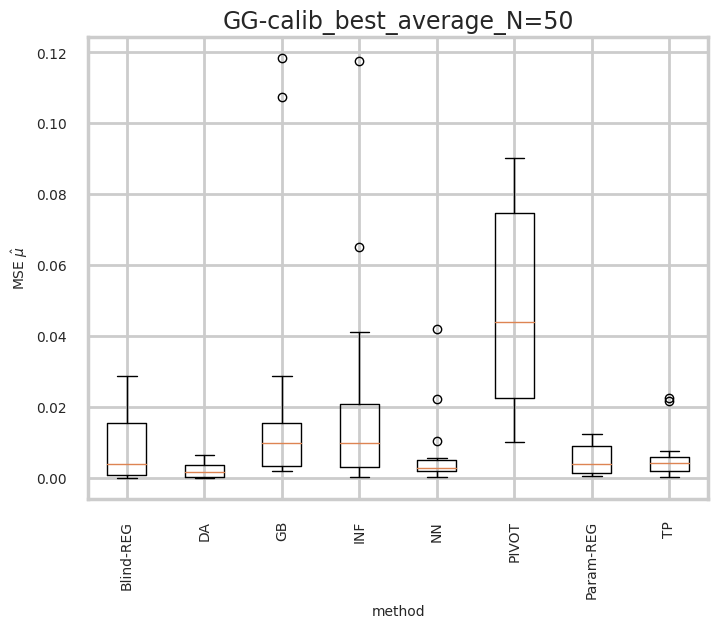
\includegraphics[width=\linewidth]{COMPARE/GG-calib/BEST_MSE/GG-calib_best_average_N=50-boxplot_mse.png}
    \caption{Boxplot of MSE on Calibrated GG}
    % \label{fig:gg-prior_best_average_boxplot_mse}
  \end{subfigure}%
  \hfill
  \begin{subfigure}[t]{0.49\linewidth}
    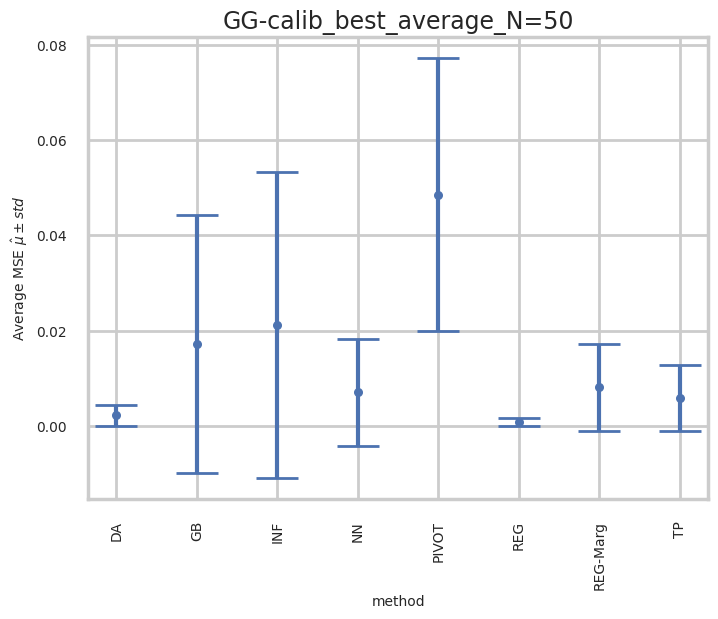
\includegraphics[width=\linewidth]{COMPARE/GG-calib/BEST_MSE/GG-calib_best_average_N=50-errplot_mse.png}
    \caption{Average MSE $\pm$ variance on Calibrated GG}
    % \label{fig:gg-calib_best_average_errplot_mse_}
  \end{subfigure}

  \caption{Best MSE on GG with 50 test samples. Distribution according to $\mu^\star$ and $\alpha^\star$.}
  \label{fig:compare_gg_best_mse50_samples}
\end{figure}


\victor{TODO : ajouter les méthodes qui utilisent la vrai likelihood et Bayes.}




\subsection{V stat and V syst} % (fold)
\label{sub:v_stat_and_v_syst}

Stuff about v stat and v syst.

Inferno is bad at v stat but always the best at v syst !
















\section{Real data} % (fold)
\label{sec:real_data}


\victor{Find out why this is does not work : \url{https://arxiv.org/pdf/1909.03081.pdf} ??}
\victor{La simulation est trop précise. cf resultat sur l'impossibilité de séparer les domaines créé}








\subsection{Nothing beats the baseline} % (fold)
\label{sub:nothing_beats_the_baseline}

\content{Show results on Higgs}







\subsection{Impossible to separate between domains} % (fold)
\label{sub:impossible_to_separate_between_domains}

\content{Show results of classifier trying to separate events between "extreme" values of nuisance params}









\subsection{Results with or without calibration} % (fold)
\label{sub:results_with_or_without_calibration}

\content{Compare results with or without using the current data in the calibration}







\subsection{Too rare signals} % (fold)
\label{sub:too_rare_signals}


\content{Explain and show that the issue comes from the imbalance between signals and backgrounds}

The scatter plot properties is much more dependent to noise or nuisance parameters than to the parameter of interest.



 %Direct regression
%!TEX root = ../thesis.tex
%*******************************************************************************
%****************************** sixth Chapter **********************************
%*******************************************************************************
\chapter{Discussion and conclusion}
\label{chap:conclusion}
% **************************** Define Graphics Path **************************
\ifpdf
    \graphicspath{{Chapter6/Figs/Raster/}{Chapter6/Figs/PDF/}{Chapter6/Figs/}}
\else
    \graphicspath{{Chapter6/Figs/Vector/}{Chapter6/Figs/}}
\fi


\victor{L'idée que c'est un graphical model mais les z sont dans le simulateur}
\victor{L'idée que si c'est sans params de nuisance alors c'est trop facile. On aurait que l'erreur statistique. On ne peut l'améliorer qu'en améliorant le classifieur. D'où vient la variance alors ?}
\victor{Sur les vrais données on doit utiliser une méthode numérique}
\victor{Quel est le budget accessible ? Combien coute la méthode normale en théorie et dans la vrai vie ? On refait vraiment tourner la simulation à chaque fois ? Combien coute ma méthode ?}
\victor{Neural network as Estimator \& estimate its variance}


\section{Calibration} % (fold)
\label{sec:calibration}

\subsection{Common calibration} % (fold)
\label{sub:common_calibration}


Multiple study using data comming from the same experiment should have the same nuisance parameter estimation.




\subsection{Prior vs posterior} % (fold)
\label{sub:prior_vs_posterior}

\content{Show the difference between the 2 formulas}
\content{The posterior of one is the prior of others}





\subsection{Update calibration} % (fold)
\label{sub:update_calibration}

Should we use the data to improve inference on the nuisance parameters ?

Technically maximum likelihood inference is doing it through maximizing the likelihood.
\victor{Oui ça semble être une totologie mais en fait c'est pas évident}


\section{Further works} % (fold)
\label{sec:further_works}

Ideas for the next steps

\subsection{Real simulator} % (fold)
\label{sub:real_simulator}

Use a real simulator instead of a trick to get a fast simulator.
Improve it with minong gold idea if possible.
Add calibration steps in the simulation.

This way the entire workflow is under control and monitoring.



\subsection{Estimate the progression margin} % (fold)
\label{sub:estimate_the_progression_margin}

Ideas to find a method to measure the maximum information that can be extracted from the given data.






 %resultats
%%!TEX root = ../thesis.tex
%*******************************************************************************
%****************************** Third Chapter **********************************
%*******************************************************************************
\chapter{Behind the scene}
\label{chap:behind}
% **************************** Define Graphics Path **************************
\ifpdf
    \graphicspath{{Chapter7/Figs/Raster/}{Chapter7/Figs/PDF/}{Chapter7/Figs/}}
\else
    \graphicspath{{Chapter7/Figs/Vector/}{Chapter7/Figs/}}
\fi

% The detailed plan is prospective at this stage


% Find a few meta parameter to evaluate the performances, and explain why it varies like that
% \begin{itemize}
% \item "learning curve" depending on number of training domain seen
% \item number of guided dropout block added
% \item show some experiments on simplified grid without production disconnections
% \item Une expérience d'apprentissage que j'aimerai voir et qui me semblerait être une bonne illustration de ce que permet l'architecture GD: montrer qu'il est possible d'apprendre incrémentalement ou séquentiellement de nouvelles conditions unitaires par rapport à un modèle déjà appris autour de conditions existantes, avec d'aussi bonnes perfs qu'un apprentissage où tout est réappris jointement sur un gros volume de données (Antoine)
% \end{itemize}

\section{Description of the data} %resultats
%%!TEX root = ../thesis.tex
%*******************************************************************************
%****************************** Third Chapter **********************************
%*******************************************************************************

\chapter{Conclusion and discussion}
\label{chap:discussion}
% **************************** Define Graphics Path **************************
\ifpdf
    \graphicspath{{Chapter8/Figs/Raster/}{Chapter8/Figs/PDF/}{Chapter8/Figs/}}
\else
    \graphicspath{{Chapter8/Figs/Vector/}{Chapter8/Figs/}}
\fi

\section{A}
\subsection{A.1} 
\subsection{A.2} 
\section{B}
\subsection{B.1} 
\subsection{B.2} 
\section{C}
\subsection{C.1} 
\subsection{C.2} 
\section{D}
\subsection{D.1} 
\subsection{D.2} 
 %conclusion and further work





% ********************************** Back Matter *******************************
% Backmatter should be commented out, if you are using appendices after References
%\backmatter

% ********************************** Bibliography ******************************
\begin{spacing}{0.9}

% To use the conventional natbib style referencing
% Bibliography style previews: http://nodonn.tipido.net/bibstyle.php
% Reference styles: http://sites.stat.psu.edu/~surajit/present/bib.htm

\bibliographystyle{apalike}
%\bibliographystyle{unsrt} % Use for unsorted references  
%\bibliographystyle{plainnat} % use this to have URLs listed in References
\cleardoublepage
\bibliography{References/references} % Path to your References.bib file


% If you would like to use BibLaTeX for your references, pass `custombib' as
% an option in the document class. The location of 'reference.bib' should be
% specified in the preamble.tex file in the custombib section.
% Comment out the lines related to natbib above and uncomment the following line.

%\printbibliography[heading=bibintoc, title={References}]


\end{spacing}

% ********************************** Appendices ********************************

\begin{appendices} % Using appendices environment for more functunality

%!TEX root = ../thesis.tex
% ******************************* Thesis Appendix A ****************************
\ifpdf
    \graphicspath{{Appendix1/Figs/Raster/}{Appendix1/Figs/PDF/}{Appendix1/Figs/}}
\else
    \graphicspath{{Appendix1/Figs/Vector/}{Appendix1/Figs/}}
\fi

\chapter{Experimental details} 


Here is gathered the details of the experiment to help reproduce the esulst prpesented in this document.


\section{What distinguish runs} % (fold)
\label{sec:what_distinguish_runs}

There is several way of estimating the parameter of interest.
These ways may differ from each other because of the pipeline, classifier training, architecture, hyper-parameters and cross-validation.
The experiments are organized as follow.

A \textbf{run} is a combinason of a \emph{problem}, a \emph{method}, a \emph{calibration}, a set of \emph{hyper-parameters}, a \emph{cross-validation} seed, and a set of \emph{true parameter}.

A \textbf{problem} is a generative process with a mixture coefficient to be infered.
Problems are assumed to be completelly determined by a set of input parameters including the parameter of interest.
The parameter of interest is the mixture coefficient or a quantity link to it by a bijective function.
List :
\begin{itemize}
	\item Gamma-Gauss [GG] : a 1D toy (see \autoref{sub:toy_1d})
	\item Synthetic 3D data [S3D2] : a replication of the 3D toy in the inferno paper (see \autoref{sub:toy_3d})
	\item Higgs ML data [HIGGS] : the data from higgsML challenge + the re-simulator (see \autoref{sec:higgs_data})
\end{itemize}

A \textbf{dataset} is a finite sampled realization of a problem given some \textbf{input parameters}.
The \textbf{nominal dataset} is a dataset produced with the most probable input parameters according to our prior knowledge.
Our prior knowledge usually consist of the calibration output and previous experiments.


A \textbf{method} is represented by a training algorithm and a pipeline.
Actually once the training algorithm is chosen there is only one pipeline that fits with the produced model.
Indeed classifiers can only use the classic worklow with maximum likelihood (see \autoref{sub:workflow}) and regressor can only use the direct approach (see \autoref{chap:direct_approach}).

List of every methods :
\begin{itemize}
	\item Gradient Boosting [GB] : a gradient boosting classifier from scikit-learn trained on the nominal data.
	\item Neural Network Classifier [NN] : a neural network trained as a classifier trained on the nominal data.
	\item Data augmentation [DA] : a neural network classifier trained on a mixture of simulated data with 1000 differents input parameters.
	\item Tangent Propagation [TP] : a neural network classifier with the tangent propagation regularization.
	\item Pivotal neural network [Pivot] : a neural network classifier with adversarial training.
	\item Inferno [INFERNO] : a neural network summary computer trained with inferno method.
	\item Regressor [REG] : a dataset wise mixture density neural network regressor taking both the data and nuisance parameter as input.
	\item Marginal Regressor [REG-Marginal] : a dataset wise mixture density neural network regressor taking only the data as input.
\end{itemize}

On a second level is the \textbf{calibration} restriction.
All method at some points requires information about the nuisance parameters.
The regressor requires to sample the nuisance parameters from a distribution for marginalization.
The optimizer requires initial values and uncertainty for all parameters and the likelihood also include constrains on the nuisance parameters.
The experiments test two calibration : the given prior knowledge and the estimation of the nuisance parameters on the test data using previously trained regressors.
Method names are decorated with "-Prior" or "-Calib" (exm : GB-Prior, REG-Calib). The marginal regressor is not concerned since it is not using calibration at all.
More realistic calibrations are left for future work.

On a third level is the \textbf{hyper-parameters} and \textbf{architecture} of the models.
The hyper-parameter setting is quite straitforward : a grid search on the most relevant hyper-parameters is done.
The resolution of the grid is quite low to avoid the need of expensive computing ressources.
The architecture choice is more complicated since there is an infinite way of desining one.
It is devellopped in a later section\needcite.

The experiments are reapeated several times to accuratelly measure the variance of the performances according to data sampling.
This is called \textbf{cross-validation} in this document although it is not allways a crossing of bunches of the same dataset as in classic cross-validation practices.
Three datasets are used in the process.
The \emph{training} set is the data used to train our model.
The \emph{validation} set is the data used to produce summary statistics (is it the azimov dataset ?).
The \emph{test} set is the data on which inference is done.

On the toy problems the generative process is cheap.
Toy datasets are generated as required and a change of the \emph{seed} is creating new train, valid and test sets.
On the higgsML data the data is first randomly splited into 3 sets see \autoref{sub:fast_re_simulator} for the details.

The final level is the choice of the \textbf{true parameters} used to generate the test set.
A combinatorial grid of possible parameters is the simplest choice to study their influence on the performances.
Again to avoid too expensive computation due to combinatorial explosion the true values of the nuisance parameters takes only 3 values :
the nominal - deviation, nominal and nominal + deviation.
The parameter of interest may be given more values.
Finally the number of samples in the test set is also evolving to measure its impact on the quality of the inference.

\victor{Ecrire exactement la variabilité restante : le train set, le test set et l'initialisation des NN}

\section{Measured quantities for performance evaluation} % (fold)
\label{sec:measured_quantities_for_performance_evaluation}


Here is given more details than in \autoref{sec:evaluation_metric}.
\victor{Donc il faudra probablement en injecter une bonne partie dans \autoref{sec:evaluation_metric} à terme.}
For each set of \emph{true parameters} several performances metrics are measured.
\victor{True parameters : donner la définition des paramètres ie $\mu$ et $\alpha$}

The main performance evaluation is the \emph{mean squared error} on the two estimated quantities : the parameter of interest and its confidence interval.
\victor{Définition de confidence interval comme interval centré (50\% à droite et à gauche)}
There is two sources of randomness in the estimated values.
The first one is the variance of the nuisance parameters which all methods is supposed to handle and include in its estimated a variance or a confidence interval of the estimated parameter of interest $\hshmu$.
The second is the data sampling which is empirically measured by repeating the experiment with cross-validation.
Altough the given variance/CL $\hshmu$ is assumed to be correct the variance of $\hmu$ is measured for comparison.
\victor{Oui mais du coup ces 2 quantités ne mesure pas vraiment la même chose, si ?}


Recall that :
\begin{eqnarray}
\label{eq:total_variance_law_2}
    \VV[Y] =& \EE_X \left (\VV[Y|X] \right ) &+ \VV_X \left (\EE[Y|X]\right ) \\
    \VV[Y] =& \EE_X \left (\VV[Y|X] \right ) &+ \EE_X \left ( (\EE [Y|X]  - \EE[Y])^2\right )
\end{eqnarray}
Giving :
\begin{equation}
\label{eq:stat_and_syst_variance_definition_2}
\mathbb{V}[\hat \mu] 
	= \underbrace{\mathbb{E}_{\alpha \sim p(\alpha)} \left (\mathbb{V}[\hat \mu, \alpha] \right )}_{V_{stat}} 
	+ \underbrace{\mathbb{V}_{\alpha \sim p(\alpha)} \left ( \mathbb{E} [\hat \mu, \alpha] \right )}_{V_{syst}}
\end{equation}
\victor{Voilà c'est là que j'ai un doute. Mon interrogation est sur la distribution de $\alpha$, on prend $p(\alpha | D)$ ou bien $p(\alpha)$ ? }
The variance can be splitted between the part coming from the nuisance parameter and the part coming from the data sampling.
The inference done asuming the value of $\alpha$ is known with $\alpha$ varying along a regular grid.
To see the influence of nuisance parameters on the inference but also to compute $V_{stat}$ and $V_{syst}$ assuming a uniform prior on $\alpha$.

Moreover we expect $V_{stat}$ to decerase in $\mathcal O \frac{1}{\sqrt{\#samples}}$ and $V_{syst}$ to be quite independant from $\#samples$.

The number predictions made by the model is also reported as a proxy of computation cost.















\section{Details} % (fold)
\label{sec:details}

Here are given the details to be able to reproduce the experiments.

\subsection{Global constants} % (fold)
\label{sub:global_constants}

The chosen global seed is 42.
This number has become famous with the popularity of H2G2\needcite.
I've seen it used quite often in codes as an easter egg.


The number of cross-validation is always 30.



\subsection{List of methods} % (fold)
\label{sub:list_of_methods}


Here is the list of all methods with a short description and their short names.
\begin{itemize}
	\item Gradient Boosting [GB] : a gradient boosting classifier from scikit-learn trained on the nominal data.
	\item Neural Network Classifier [NN] : a neural network trained as a classifier trained on the nominal data.
	\item Data augmentation [DA] : a neural network classifier trained on a mixture of simulated data with 1000 differents input parameters.
	\item Tangent Propagation [TP] : a neural network classifier with the tangent propagation regularization.
	\item Pivotal neural network [Pivot] : a neural network classifier with adversarial training.
	\item Inferno [INFERNO] : a neural network summary computer trained with inferno method.
	\item Regressor [REG] : a dataset wise mixture density neural network regressor taking both the data and nuisance parameter as input.
	\item Marginal Regressor [REG-Marginal] : a dataset wise mixture density neural network regressor taking only the data as input.
\end{itemize}



\subsection{Neural network architectures} % (fold)
\label{sub:neural_network_architectures}


The choice of neural network architecture is a critical hyper-parameter but also the most difficult to tune because of its complexity.
Automatization of neural network architecture search is still an open problem \needcite.
Although better architectures will leads to better performances, neural network architecture is not the focus of this study.
To give a fair comparison between methods at an affordable computation cost the chosen architectures are splited into 3 classes.

\emph{Small} architectures to give base performances of maybe undersized networks.
\emph{Large} architectures are expected to provide good if not best performances.
\emph{Huge} architecture which are deliberately over-sized to make sure that bigger won't be better.


Each layers have the exact same amount of neurons which is the only hyper-parameter of the architecture.
In hope to better limit the inlfuence of the architecture on the performances residual conections are used in large network.
Networks are built using simple blocs :
\begin{itemize}
	\item \textbf{Linear} layers are simple neural networks $o = W.x + b$
	\item \textbf{Residual} blocs are 2 simple layers with an intermediate space half the size of the input and separated with an activation. $o = x + W_2 . a(W_1.x + b)$
	\item \textbf{Average} layers are described \autoref{sub:datasetwise_input} $o = U.X+b+V.r(X)$
	\item \textbf{Residual Average} blocs are 2 average layers with an intermediate space half the size of the input and separated with an activation. $o^\prime = a( U_1.X+b+V_1.r(X) )$ and $o = x + U_2.o^\prime + V_2.r(o^\prime) $
\end{itemize}
Making the intermediate space half the size of the input in residual blocs is assumed to encourage the network to learn simpler functions.
This way the residual blocs are learning a simple correction of the input.
Chaining these corrections should allow the network to produce arbitrarily complex functions but encourage it toward ones close to a linear function.

All architectures names follow a simple code :
\begin{itemize}
	\item L = Linear
	\item R = Residual block
	\item M = Mean operation (reduction)
	\item A = Average layer
	\item AR = Average Residual block
\end{itemize}
Followed by a number representing the number of layers.
Since residual blocs includes 2 layers a single residual bloc is always followed by a even number representing twice the number of blocs.

The classic architectures is used for classifiers
\begin{itemize}
	\item \textbf{L4} [small] : simple feed forward neural network with 4 layers with ReLU activations.
	\item \textbf{L1R8L1} [large] : a linear layer followed by 4 residual blocs and a final linear layer.
	\item \textbf{L1R20L1} [huge] : a linear layer followed by 10 residual blocs and a final linear layer.
\end{itemize}

The average architectures is an addition to INFERNO.
INFERNO training can leverage the datasetwise architecture so additional architectures were included to see what happens.
\begin{itemize}
	\item \textbf{L1A2L1} [small] : a linear layer followed by 2 average layers and a final linear layer.
	\item \textbf{A1AR8L1} [large] : an average layer followed by 4 average residual blocs and a final linear layer.
	\item \textbf{A1AR20L1} [huge] : an average layer followed by 10 average residual blocs and a final linear layer.
\end{itemize}

The regressor architectures are a bit bigger because the learned functions are expected to be more complex.
\begin{itemize}
	\item \textbf{A3ML3} [small] : 3 average layers an average reduction and 3 linear layers.
	\item \textbf{A1AR2ML1} [small] : an average layer followed by 1 average residual bloc, an average reduction and a final linear layer.
	\item \textbf{A1AR8MR8L1} [large] : an average layer followed by 4 average residual blocs then an average reduction followed by 4 residual blocs and a final linear layer.
	\item \textbf{A1AR18MR4L1} [huge] : an average layer followed by 9 average residual blocs, an average reduction followed by 2 residual blocs and a final linear layer.
\end{itemize}

Finaly the choice of activation determines the smoothness of a network.
Only relying on ReLU will likely end in a piecewise linear function while a sigmoid of tanh activation may lead more curves.
Morover ReLU is never saturating which led to some gradient explosion is preliminary experiments. 
To avoid having to test many activations the default activation is applying ReLU6 to the first half of the neurons and tanh to the rest of the neurons.
This is assumed to allow the network to use the best of both world.






\subsection{Hyper-parameter grid} % (fold)
\label{sub:hyper_parameter_grid}

\content{Donner la grille pour chaque modèle et \textbf{expliquer pourquoi ces HP sont choisis}}


\begin{table}[ht!]
\centering
\begin{tabular}{||c c c c||} 
 \hline
 \multicolumn{4}{|c|}{Gradient boosting}\\
 \hline
 Problem & GG & S3D2 & HiggsML \\ [0.5ex] 
 \hline
 \# estimators & [100, 300, 1000] & [100, 300, 1000] & [500, 1000, 2000] \\ 
 max-depth     & [3, 5, 10] & [3, 5, 10] & [3, 5, 10] \\
 learning-rate & [0.1, 0.05, 0.01] & [0.1, 0.05, 0.01] & [0.1, 0.05, 0.01] \\
 \hline
\end{tabular}
\caption{Table of hyper-parameters for Gradient boosting}
\label{table:HP_GB}
\end{table}


\begin{table}[ht!]
\centering
\begin{tabular}{||c c c c||} 
 \hline
 \multicolumn{4}{|c|}{Neural network classifier}\\
 \hline
 Problem & GG & S3D2 & HiggsML \\ [0.5ex] 
 \hline
 \# units & [50, 100, 200, 500] & [50, 100, 200, 500] & [50, 100, 200, 500] \\ 
 \# steps & [2000, 5000] & [2000, 5000] & [2000, 5000, 10 000] \\
 batch-size &  20 &  20 & 20 \\
 learning-rate & [1e-3] & [1e-3] & [1e-3] \\
 Optimizer & Adam & Adam & Adam \\
 $\beta_1$ & 0.9 & 0.9 & 0.9 \\
 $\beta_2$ & 0.999 & 0.999 & 0.999 \\
 \hline
\end{tabular}
\caption{Table of hyper-parameters for Neural network classifier}
\label{table:HP_NN}
\end{table}


\begin{table}[ht!]
\centering
\begin{tabular}{||c c c c||} 
 \hline
 \multicolumn{4}{|c|}{Data Augmentation}\\
 \hline
 Problem & GG & S3D2 & HiggsML \\ [0.5ex] 
 \hline
 \# units & [50, 100, 200, 500] & [50, 100, 200, 500] & [50, 100, 200, 500] \\ 
 \# steps & [2000, 5000] & [2000, 5000] & [2000, 5000, 10 000] \\
 batch-size &  20 &  20 & 20 \\
 learning-rate & [1e-3] & [1e-3] & [1e-3] \\
 Optimizer & Adam & Adam & Adam \\
 $\beta_1$ & 0.9 & 0.9 & 0.9 \\
 $\beta_2$ & 0.999 & 0.999 & 0.999 \\
 \hline
\end{tabular}
\caption{Table of hyper-parameters for Data Augmentation}
\label{table:HP_DA}
\end{table}


\begin{table}[ht!]
\centering
\begin{tabular}{||c c c c||} 
 \hline
 \multicolumn{4}{|c|}{Tangent propagation}\\
 \hline
 Problem & GG & S3D2 & HiggsML \\ [0.5ex] 
 \hline
 \# units & [50, 100, 200, 500] & [50, 100, 200, 500] & [50, 100, 200, 500] \\ 
 \# steps & [2000, 5000] & [2000, 5000] & [2000, 5000, 10 000] \\
 batch-size &  20 &  20 & 20 \\
 learning-rate & [1e-3] & [1e-3] & [1e-3] \\
 Optimizer & Adam & Adam & Adam \\
 $\beta_1$ & 0.9 & 0.9 & 0.9 \\
 $\beta_2$ & 0.999 & 0.999 & 0.999 \\
 trade-off & [1, 0.1, 1e-2, 1e-3] & [1, 0.1, 1e-2, 1e-3] & [1, 0.1, 1e-2, 1e-3] \\
 \hline
\end{tabular}
\caption{Table of hyper-parameters for Tangent Propagation}
\label{table:HP_TP}
\end{table}


\begin{table}[ht!]
\centering
\begin{tabular}{||c c c c||} 
 \hline
 \multicolumn{4}{|c|}{Pivot}\\
 \hline
 Problem & GG & S3D2 & HiggsML \\ [0.5ex] 
 \hline
 \# units & [50, 100, 200, 500] & [50, 100, 200, 500] & [50, 100, 200, 500] \\ 
 \# steps & [2000, 5000] & [2000, 5000] & [2000, 5000, 10 000] \\
 batch-size &  20 &  20 & 20 \\
 learning-rate & [1e-3] & [1e-3] & [1e-3] \\
 Optimizer & Adam & Adam & Adam \\
 $\beta_1$ & 0.9 & 0.9 & 0.9 \\
 $\beta_2$ & 0.999 & 0.999 & 0.999 \\
 trade-off & [1, 0.1, 1e-2, 1e-3] & [1, 0.1, 1e-2, 1e-3] & [1, 0.1, 1e-2, 1e-3] \\
 \hline
\end{tabular}
\caption{Table of hyper-parameters for Pivot}
\label{table:HP_PIVOT}
\end{table}


\begin{table}[ht!]
\centering
\begin{tabular}{||c c c c||} 
 \hline
 \multicolumn{4}{|c|}{INFERNO}\\
 \hline
 Problem & GG & S3D2 & HiggsML \\ [0.5ex] 
 \hline
 \# units & [50, 100, 200, 500] & [50, 100, 200, 500] & [50, 100, 200, 500] \\ 
 \# steps & [2000, 5000] & [2000, 5000] & [2000, 5000, 10 000] \\
 batch-size &  1 &  1 & 1 \\
 sample-size &  1000 &  1000 & 1000 \\
 learning-rate & [1e-3] & [1e-3] & [1e-3] \\
 Optimizer & Adam & Adam & Adam \\
 $\beta_1$ & 0.5 & 0.5 & 0.5 \\
 $\beta_2$ & 0.9 & 0.9 & 0.9 \\
 temperature & 1 & 1 & 1 \\
 \hline
\end{tabular}
\caption{Table of hyper-parameters for INFERNO}
\label{table:HP_INF}
\end{table}



\begin{table}[ht!]
\centering
\begin{tabular}{||c c c c||} 
 \hline
 \multicolumn{4}{|c|}{Regressor}\\
 \hline
 Problem & GG & S3D2 & HiggsML \\ [0.5ex] 
 \hline
 \# units & [50, 100, 200, 500] & [50, 100, 200, 500] & [50, 100, 200, 500] \\ 
 \# steps & [2000, 5000] & [2000, 5000] & [2000, 5000, 10 000] \\
 batch-size &  1 &  1 & 1 \\
 sample-size &  1000 &  1000 & 1000 \\
 learning-rate & [1e-3] & [1e-3] & [1e-3] \\
 Optimizer & Adam & Adam & Adam \\
 $\beta_1$ & 0.5 & 0.5 & 0.5 \\
 $\beta_2$ & 0.9 & 0.9 & 0.9 \\
 \hline
\end{tabular}
\caption{Table of hyper-parameters for Neural network datasetwise regressor}
\label{table:HP_REG}
\end{table}





\subsection{True parameter grid} % (fold)
\label{sub:true_parameter_grid}


\begin{table}[ht!]
\centering
\begin{tabular}{||c c||} 
 \hline
 \multicolumn{2}{|c|}{1D Toy GG true parameter grid}\\
 \hline
 $\mu$ & [0.1, 0.3, 0.5, 0.7, 0.9] \\ 
 $\alpha$ & [0.8, 1. , 1.2] \\ 
 \hline
\end{tabular}
\caption{Table of true parameter grid for the 1D Toy GG}
\label{table:GG_true_grid}
\end{table}

The fine range of $\alpha$ for systematic/statistical variance estimation is 31 equidistant values in $[0.5, 1.5]$ . 


\subsection{Prior distributions} % (fold)
\label{sub:prior_distributions}


\victor{TODO !}



\subsection{Data size} % (fold)
\label{sub:data_size}


\begin{table}[ht!]
\centering
\begin{tabular}{||c c c c||} 
 \hline
 \multicolumn{4}{|c|}{Data size}\\
 \hline
 Problem & GG & S3D2 & HiggsML \\ [0.5ex] 
 \hline
 \# training samples & 10 000 & 30 000 & ?? \\ 
 \# validation samples & 5 000 & 30 000 & ?? \\
 \# test samples & [50, 100, 300, 500, 2000] & [??] & [??] \\
 \hline
\end{tabular}
\caption{Table of the base number of samples in training, validation or testing datasets. }
\label{table:data_sizes}
\end{table}






%!TEX root = ../thesis.tex
% ******************************* Thesis Appendix B ********************************

\ifpdf
    \graphicspath{{Appendix2/Figs/Raster/}{Appendix2/Figs/PDF/}{Appendix2/Figs/}}
\else
    \graphicspath{{Appendix2/Figs/Vector/}{Appendix2/Figs/}}
\fi

\chapter{Lost and found}

\content{Details, sections and parts that do not fit the current plan}


\section{Simulator limitation} % (fold)
\label{sec:simulator_limitation}

Est si tout ces problèmes c'était parce que le simulateur ne va pas ? cf p(nuisance | data) vs p(nuisance) ... ???
% section simulator_limitation (end)

\section{Chap1-old Background}


\subsection{High energy physics} % (fold)
\label{sub:high_energy_physics}

\subsection{CERN} % (fold)
\label{sub:cern}


\subsection{Systematics} % (fold)
\label{sub:systematics}



\section{Chap1-old Motivation} % (fold)
\label{sec:motivation}

Limitations des méthodes actuelles

\subsection{Accuracy} % (fold)
\label{sub:accuracy}


\subsection{computation} % (fold)
\label{sub:computation}

\subsection{Understanding and methodology} % (fold)
\label{sub:understanding_and_methodology}

Levée de confusion entre mesure et découverte.

Évaluation quantitative empirique des résultats => test statistique "non parametrique"

+ justifications théorique




\section{ TODO Papers }

Found this paper \url{https://arxiv.org/pdf/1903.10563.pdf} which review ML + Physics.

So let's dive into the state of the art of inference in Physics using ML.
Especially in the inverse problem setting.

\begin{itemize}
    \item \url{https://arxiv.org/abs/1506.02169} : Approximating Likelihood Ratios with Calibrated Discriminative Classifiers
    \item \url{https://arxiv.org/abs/1601.07913} : Parameterized Machine Learning for High-Energy Physics
    \item \url{https://arxiv.org/abs/1610.08328} : Event generator tuning using Bayesian optimization
    \item \url{https://arxiv.org/abs/1611.01046} : Learning to Pivot with Adversarial Networks
    \item \url{https://arxiv.org/abs/1706.04008} : Recurrent Inference Machines for Solving Inverse Problems
    \item \url{https://arxiv.org/abs/1707.07113} : Adversarial Variational Optimization of Non-Differentiable Simulators
    \item \url{https://arxiv.org/abs/1801.01497} : Massive optimal data compression and density estimation for scalable, likelihood-free inference in cosmology
    \item \url{https://arxiv.org/abs/1802.03537} : Automatic physical inference with information maximising neural networks
    https://arxiv.org/abs/1805.03961
    \item \url{https://arxiv.org/abs/1805.03961} : Study of constraint and impact of a nuisance parameter in maximum likelihood method
    \item \url{https://arxiv.org/abs/1805.07226} : Sequential Neural Likelihood: Fast Likelihood-free Inference with Autoregressive Flows
    \item \url{https://arxiv.org/abs/1805.00020} : A Guide to Constraining Effective Field Theories with Machine Learning
    \item \url{https://arxiv.org/abs/1805.00013} : Constraining Effective Field Theories with Machine Learning
    \item \url{https://arxiv.org/abs/1805.12244} : Mining gold from implicit models to improve likelihood-free inference
    \item \url{https://arxiv.org/abs/1806.11484} : Deep Learning and its Application to LHC Physics
    \item \url{https://arxiv.org/abs/1903.01473} : Nuisance hardened data compression for fast likelihood-free inference
    \item \url{} : 
    \item \url{} : 
    \item \url{} : 
    \item \url{https://cds.cern.ch/record/1099977/files/p111.pdf} : Computing Likelihood Functions for High-Energy Physics Experiments when Distributions are Defined by Simulators with Nuisance Parameters
    \item \url{https://arxiv.org/abs/1007.1727} : Asymptotic formulae for likelihood-based tests of new physics
    \item \url{https://www.pp.rhul.ac.uk/~cowan/stat/aachen/cowan_aachen14_1.pdf} : Cours de Glen 2012 part 1
    \item \url{https://www.pp.rhul.ac.uk/~cowan/stat/aachen/cowan_aachen14_2.pdf} : Cours de Glen 2012 part 2
    \item \url{https://www.pp.rhul.ac.uk/~cowan/stat/aachen/cowan_aachen14_3.pdf} : Cours de Glen 2012 part 3
    \item \url{https://www.pp.rhul.ac.uk/~cowan/stat/aachen/cowan_aachen14_4.pdf} : Cours de Glen 2012 part 4
    \item \url{https://www.pp.rhul.ac.uk/~cowan/stat/aachen/cowan_aachen14_5.pdf} : Cours de Glen 2012 part 5
    \item \url{https://arxiv.org/pdf/1503.07622.pdf} : Practical Statistics for the LHC
    \item \url{} : 
    \item \url{} : 
    \item \url{} : 
    \item \url{} : 
\end{itemize}


\section{ ABC }

Approximate Bayesian Computation is ...

\section{ Inferno }
\section{ Learning to become }

\section{ Mining gold }

\begin{itemize}
	\item The paper for Machine learner  : https://arxiv.org/abs/1805.12244
	\item The paper for physicist : https://arxiv.org/abs/1805.00013 and https://arxiv.org/abs/1805.00020
	\item The ALICES paper : https://arxiv.org/pdf/1808.00973.pdf
    \item The general paper about simulation base inference ! https://arxiv.org/pdf/1911.01429.pdf
\end{itemize}

Augment the simulated data with the likelihood ratio ...





\section{Disentangling} % (fold)
\label{sec:disentangling}


\begin{itemize}
    \item \url{https://arxiv.org/pdf/1611.03383.pdf} : Disentangling factors of variation in deep representations using adversarial training
    \item \url{https://arxiv.org/pdf/1811.12359.pdf} : Challenging Common Assumptions in the Unsupervised Learning of Disentangled Representations
\end{itemize}



\section{Variational} % (fold)
\label{sec:variational}

\begin{itemize}
    \item \url{https://arxiv.org/pdf/1601.00670.pdf} : Variational Inference: A Review for Statisticians
    \item \url{} : VAE with a VampPrior
\end{itemize}


\section{Uncertainty} % (fold)
\label{sec:uncertainty}

\begin{itemize}
    \item \url{https://arxiv.org/pdf/1906.02530.pdf} : Can You Trust Your Model's Uncertainty? Evaluating Predictive Uncertainty Under Dataset Shift
\end{itemize}




\section{Introduction} % (fold)
\label{sec:introduction}

\begin{itemize}
	\item \url{https://www.osti.gov/servlets/purl/1469751} Nature paper about how much ML help HEP.
\end{itemize}


\section{Plan and structure} % (fold)
\label{sec:plan_and_structure}

Suivant le conseil de François je commence par le "steak", ie ce dont je veux parler / les sujets principaux du manuscrit.

\textbf{Contributions :}
\begin{itemize}
    \item Décrire certaines limites de l'adaptation de domaine pour réduire l'influence des effets systeméatiques
    \item (Application de la regression directe sur un dataset pondéré à HEP)
    \begin{itemize}
        \item inspiration : PointNet, papier de correntin, Neural statistician, papier de Théo (bio-stat en général) ?
    \end{itemize}
    \item Décrire certaines limites à l'inférence par régression directe
\end{itemize}


\textbf{Pour pouvoir en parler je dois introduire :}
\begin{itemize}
    \item Un tout petit peu de physique
    \begin{itemize}
        \item description minimaliste du systeme
        \item mais quand même insister sur le fait que c'est bien + compliqué
    \end{itemize}
    \item Les techniques d'inférence
    \begin{itemize}
        \item Inférence bayesienne
        \item maximum de vraisemblance
    \end{itemize}
    \item Le probleme inverse
    \item Les effets systématiques et leur conséquence
\end{itemize}

\textbf{Il faut aussi parler des solutions actuelles et autres empreints à la litterature}
\begin{itemize}
    \item data augmentation
    \item tangent propagation
    \item pivot
    \item inferno
\end{itemize}

\textbf{Que je me positionne par rapport à d'autres alternatives non explorées:}
\begin{itemize}
    \item Variationnal inference
    \item ABC methods
    \item Bayesian networks
    \item Disentagling
    \item Fairness
    \item Mining gold
\end{itemize}


\textbf{Présentation du benchmark ie des données, des XP, etc}
\begin{itemize}
    \item Présenter les jeux de données
    \begin{itemize}
        \item Toy 1D
        \item Toy inferno
        \item HiggsML
    \end{itemize}
    \item Workflow pour l'inférence
    \item Workflow pour la sélection de l'outil ie exp data = simulator($\theta^\star$) (car les données xp ne sont utilisée qu'une fois)
    \item Présenter la métrique pour comparer les méthodes
    \item Présenter les résultats sur ces données
    \begin{itemize}
        \item Tout marche bien jusqu'à un certain point
        \item Classement difficile mais : Bayes \& likelihood > classifier and inerno > direct regression
        \item Rien ne semble battre la baseline sur HiggsML
    \end{itemize}
    \item Approfondir l'interprétation de ces résultats avec les XP auxilières
    \begin{itemize}
        \item Forest robustness
        \item Toy trop facile (linear correlation with mu)
        \item No correlation with higgs
        \item Signal too weak => regression learning impossible
        \item Separation between domain in higgs very difficult (at sample size)
        \item Autres ???
    \end{itemize}
    \item Rien ne marche ici mais systematic aware learning ça marche dans d'autre cas.
\end{itemize}


\textbf{Discussion sur les limites et les perspectives}
\begin{itemize}
    \item limite minimal pour la réduction de la variance systématique (pas de démêlage parfait possible)
    \item Amélioration du simulateur
    \item Probabilistic programming ?
    \item Calibration commune pour de multiples analyses
    \item Calibration and Prior vs posterior ? (territoire glissant) 
    \item j'ai envie de donner un regard critique sur l'obscurantisme autour des statistiques
    \item j'ai envie de donner un regard critique sur la méthodologie pour mesurer les performances
\end{itemize}


\textbf{Remarques Isabelle : }
\begin{itemize}
    \item Introduire le pb du comptage bcp + tôt.
    \item Pas forcément un ordre chronologique
    \item Mais plutôt quel est ce que je veux dire et contruire autour 
    \item Résoudre le comptage et prendre en compte les systématiques
    \begin{itemize}
        \item être insensible au systématique
        \item les évaluer
        \item Il faut être clair sur ce que l'on fait avec ces systématiques
    \end{itemize}
    \item On veut sortir un $\mu$ aussi indépendant de $\alpha$ que possible
    \item Chercher en background process la punchline de ma thèse.
\end{itemize}



\section{Thoughts on calibration} % (fold)
\label{sec:thoughts_on_calibration}

According to "something-I-have-not-found-anywhere-yet" we should not use the data to infer the nuisance parameters \ie improve the calibration.
Indeed trying to narrow down the distribution of the nuisance params $p(\alpha|x)$ using the given data $x^\star$ is considered dangerous.

But I do not understand why.

Here is the problem : if the calibration is nearly perfect then $p(\alpha|x)$ is narrow (\ie very small variance) the simulation data $x|\alpha$ is close to the true data used for inference $x^\star$. Then the classifier (or any other method) output is not going to change much according to $\alpha$ because all $\alpha$ are very close to each other.

If the calibration is not perfect $p(\alpha|x)$ is not a narrow distribution. Then the simulation data $x|\alpha$ will vary enough for the classifier/method to change its output. But if the classifier can "feel it" then how the calibration does not ?


example : tau energy scale.
It is quite simple to measure the tau energy scale from the data. Take the tau feature, average it and compare to the simulation. This gives a perfect estimator of the tau enery scale. This is doing calibration on the given data $x^\star$.
I do not see how it is dangerous to rescale the data... We do it all the time in Machine Learning before doing linear regression or feeding the data to the neural network. Usually it is done sample-wise but here a sample is simply a dataset. One dataset is one $x$.


What I do understand is that the data will be used to infer many parameters in different studies. 
If all these studies uses a home made re-calibration then 2 studies using the same experiment will use different values for the nuisance param which seems foolish and can probably leads to wrong conclusions.
Example : the tau energy scale has one value (one distrib) for the entire experiment. If Paul finds 1.2 with its method and Jean find 1.1 with another method they may find different conclusion for the exact same study on the exact same data !

To avoid this problem the calibration is done in a controled region where no studies will look because other parameters have little influence there.
This should makes the calibration as powerfull as possible meaning the proba $p(\alpha|x)$ as narrow as possible.

Now we have a $p(\alpha|x)$ that should not be modified in studies using this experiment.
Meaning we cannot improve the second part of the variance : 
$$\EE_{\alpha \sim p(\alpha|x)} \left ((\EE [y|x, \alpha]  - \EE[y|x])^2\right )$$
which measures the deviation of the estimator according to the average value of the estimator.


Unless we improve the estimator itself to be resilient to change in the values of $\alpha$.

My intuition is that it is impossible if the estimator is well built (\ie not broken).
This seems to lead to the bias-variance trade-off.

$$
\VV[y|x] = \EE_{\alpha \sim p(\alpha|x)} \left (\VV[y|x, \alpha] \right ) + \EE_{\alpha \sim p(\alpha|x)} \left ( (\EE [y|x, \alpha]  - \EE[y|x])^2\right )
$$

If I improve the second term the first one (representing the average variance of the estimator) will get bigger.
In other words what we win in systematic error we will loose it in statistical error.

I get that disantangling the nuisance from the interest param is the goal. 
But I think a classifier is already doing it (probably not by chance, cross entropy is deeply linked to the objective function) in the higgs dataset.


What I still do not understand completly is why we don't improve the frozen calibration ?
According to Bayes theorem we can (carefully) improve knowledge on a parameter with multiple experiment.


If my intuition is wrong and the controled region calibration is the best way of doing calibration. 
Then all inference aware methods are dangerous since the neural network can learn to calibrate.

This is exactly what I allow my big neural net to do with all the reduction functions inside it.
And INFERNO-like methods can indeed use one bin to calibrate on the data.


Reminder of my thoughts :
\begin{itemize}
	\item Rescaling the dataset is like rescaling a feature in ML. It is not dangerous in usual ML. Is it really dangerous here ?
	\item Multiple home-made calibration on same dataset may lead to wrong conclusions
	\item Calibration done in a controled region is a workaround to freeze calibration for every study using this data
	\item Can we improve this frozen calibration ? cf bayes theorem to improve our knowledge in view of new observations
\end{itemize}



\subsection{Apple and pears} % (fold)
\label{sub:apple_and_pears}

Let's start with a toy problem and make it gradually more complex.
The study is about finding the proportion $\mu$ of apples and pears in a bag.
The only information available is the total number of fruits in the bag and the weight of each individual fruit.
Apples and pears weights are normally distributed and slightly different.
The dataset is a set of real values $D = \{ x_i \in \RR \} $

From the average weight of the fruits in the bag a linear regression is enough to find the link between $D$ and the parameter of interest $\mu$.
The model can be trained if enough bags in which the proportion is known is available for training.
This simplicity is wanted to test the method.

Since the weight of a fruit is stochastic, two bags of fruits with the same number of apples and pears may have a different average weight.
Leading to some uncertainty in the predicted proportion that must be reported.


\subsection{Simulation} % (fold)
\label{sub:simulation}


Vulgarization on atlas simulation :
\begin{itemize}
	\item \url{https://atlas.cern/updates/atlas-blog/defending-your-life-part-1}
	\item \url{https://atlas.cern/updates/atlas-blog/defending-your-life-part-2}
	\item \url{https://atlas.cern/updates/atlas-blog/defending-your-life-part-3}
\end{itemize}




\section{Math} % (fold)
\label{sec:math}

This section develops what I understand so far about the theory.
It is also an opportunity to gather all the quantities at the same place to give them unique names and notations.

For now I skip the latent variables that describes what happen between the collision and the measurement.
For now I also skip the trigger because it only add more complexity to the problem without fundamental changes.

\subsection{Notation and context} % (fold)
\label{sub:notation_and_context}

Notation :
\begin{itemize}
	\item $\alpha$ = nuisance parameter
	\item $\beta$ = poisson law parameter for the number of backgrounds
	\item $\gamma$ = Poisson law parameter for the number of signals according to current theory
	\item $\mu$ = deviation from the expected number of signals from theory
	\item $z$ or $z_i$ = latent variables describing 
	\item $n$ = number of event
	\item $s$ = number of signals
	\item $b$ = number of backgrounds
	\item p(x) = probability density of an event $x$
	\item p(x|S) = conditional probability density of an event $x$ knowing it is a signal ie signal likelihood
	\item p(x|B) = conditional probability density of an event $x$ knowing it is a background ie background likelihood
\end{itemize}

Let's consider a counting exepriment in a collider.
Inside the collider two bunch of particles are meeting at some point.
From this meeting two types of collisions are possible :
\begin{itemize}
	\item Soft collision which does not produce interesting physics
	\item Hard collision which produces interesting physics called \textbf{event}
\end{itemize}

The hard collisions (events) are way rarer than the soft one.
The process creating the high energy particles is fundamentally stochastic.
Meaning that the nature and properties (eg. kinematics) of the process producing particles are not fully predictable but follow probability distributions whose shapes and properties are deterministics.

The data can be modeled by counting iid Bernouilli rare process which is well approximated by a Poisson distribution \needcite (cf wikipedia) when the number of samples is large.
\begin{equation}
	n \sim Poisson(\text{some parameter})
\end{equation}


The events are splitted into 2 categories the background events and the background events.
The signal events are events generated with a peculiar process (e.g. $H\to \tau^+ \tau^-$) that we want to study.
The backgroud events gather all the other processes.
The expected amount of background events $\beta$ is known (with high precision) thanks previous studies/experiments and to measurements made in the data space where few or no signals can be found.



\subsection{Estimate mu in a simple case} % (fold)
\label{sub:estimate_mu_in_a_simple_case}

Let's first write everything without nuisance parameters.

The total number of events is the sum of signal events and background events.
\begin{equation}
	n = s + b
\end{equation}
The number of signal events is following a poisson distribution of parameter $\mu \gamma$.
\begin{equation}
	s \sim Poisson(\mu \gamma)
\end{equation}
The number of background events is following a poisson distribution of parameter $\beta$.
\begin{equation}
	b \sim Poisson(\beta)
\end{equation}
Since the sum of Poisson random variables is also Poisson distributed \needcite (cf wikipedia) :
\begin{equation}
	n \sim Poisson(\mu \gamma + \beta)
\end{equation}

The objective of the study is to infer $\mu$ from data.
The objective of this document is to clarify a few questions :
\begin{itemize}
	\item What is the link between the probability density of an event $p(x)$ and the number of events $n$ ?
	\item Why is it better to divide the data space into bins ?
	\begin{itemize}
		\item What is the link between signal purity (ie maximum $s/b$) and the variance of the estimator of $\mu$ ?
		\item Is it better to keep only the bin with maximum signal purity (ie maximum $s/b$) ?
		\item Is signal purity $s/b$ or $\gamma / \beta$ ? Are those definition equivalent ?
	\end{itemize}
\end{itemize}



Let's start with the link between the number of events ($s$, $b$, $n$) and the number of events in a bin ($s_i$, $b_i$, $n_i$).
A bin is a subspace of the data space where the event can appear.
We define $\Omega_i$ the subspace of the i-th bin and $\Omega_{tot} = \bigcup_i^K \Omega_i $ the full data space as the union of my $K$ bins.
Begining with the obvious quantity :
\begin{equation}
	n = |D| = \sum_{x\in D} 1
\end{equation}
The number of events in a bin is simply the fraction of events that falls inside a bin.
\begin{equation}
	n_i = \sum_{x\in D} \mathbbm{1} [x\in \Omega_i]
\end{equation}



On average (or in the infinite sample case) an event falls inside the i-th bin with probability $p(x \in \Omega_i)$ defined as:
\begin{equation}
	p(x \in \Omega_i) = \int_{x \in \Omega_i} p(x) dx
\end{equation}
Leading to :
\begin{equation}
	\label{eq:nb_events_in_bin}
	\EE [n_i] = \EE [n] \times p(x \in \Omega_i)  = \EE[n] \times \int_{x \in \Omega_i} p(x) dx
\end{equation}
Let's keep pushing open doors for clarity.
An event is either a signal event $S$ or a background event $B$.
Therefore we can decompose the density into two parts :
\begin{equation}
	p(x) = p(x|S) p(S) + p(x|B) p(B)
\end{equation}
Injecting this into \autoref{eq:nb_events_in_bin}
\begin{align}
	\EE [n_i] &= \EE[n] \times \int_{x \in \Omega_i} p(x) dx \\
	\EE [n_i] &= \EE[n] \times \int_{x \in \Omega_i} p(x|S) p(S) + p(x|B) p(B) dx \\
	\EE [n_i] &= \EE[n] \times \left ( \int_{x \in \Omega_i} p(x|S) p(S) dx + \int_{x \in \Omega_i}  p(x|B) p(B) dx \right )\\
	\EE [n_i] &= \EE[n] \times \int_{x \in \Omega_i} p(x|S) p(S) dx \quad+\quad \EE[n] \times \int_{x \in \Omega_i}  p(x|B) p(B) dx \\
	\EE [n_i] &= \EE[n] \times p(S) \int_{x \in \Omega_i} p(x|S) dx \quad+\quad \EE[n] \times p(B) \int_{x \in \Omega_i}  p(x|B) dx \\
	\EE [n_i] &= \EE[s] \int_{x \in \Omega_i} p(x|S) dx \quad+\quad \EE[b] \int_{x \in \Omega_i}  p(x|B) p(B) dx \\
\end{align}
We find that $\EE[s] = \EE[n] \times p(S)$ and $\EE[b] = \EE[n] \times p(B)$ which is again obvious statement since the expected number of signal events is the expected total number of event times the probability of an event to be a signal.
Replacing expenctancies of the number of events with their values according to our Poisson parameter
\begin{equation}
	\EE[n_i] = (\mu\gamma + \beta) \times \int_{x \in \Omega_i} p(x) dx
\end{equation}
\begin{equation}
	\EE[s_i] = \mu\gamma \times \int_{x \in \Omega_i} p(x|S) dx
\end{equation}
\begin{equation}
	\EE[b_i] = \beta \times \int_{x \in \Omega_i} p(x|B) dx
\end{equation}

The answer to the question : what is the link between $p(x)$ and $n$ is \autoref{eq:nb_events_in_bin}.





\section{Discussion sur modern ML and deep learning} % (fold)
\label{sec:discussion_sur_modern_ml_and_deep_learning}


\url{https://arxiv.org/abs/1812.11118} and 
\url{https://openai.com/blog/deep-double-descent/}

il manque neural tangeant kernel.






% Bibliography for convenience when sending appendix parts by email.
\bibliography{References/references} % Path to your References.bib file

\end{appendices}



% *************************************** Index ********************************
\printthesisindex % If index is present

%\cleardoublepage
%!TEX root = ../thesis.tex
%*******************************************************************************
%****************************** Third Chapter **********************************
%*******************************************************************************
\thispagestyle{empty}
\newgeometry{
left=12mm,
top=30mm,
right=12mm,
bottom=30mm
}

\begin{textblock*}{61mm}(16mm,3mm)
	\noindent\includegraphics[height=24mm]{ed_doc/\logoEd.jpeg}
\end{textblock*}

%\begin{changemargin}{-3cm}{-3cm}

\begin{footnotesize}
%%%Titre de la thèse en français / Thesis title in french
\begin{center}
\fcolorbox{bordeau}{white}{\parbox{0.95\textwidth}{
{\bf Titre:} \PhDTitleFR 
%\medskip

%%%Mots clés en français, séprarés par des ; / Keywords in french, separated by ;
{\bf Mots clés:} \keywordsFR 
\vspace*{-4mm}

%%% Résumé en français / abstract in french
\begin{multicols}{2}
{\bf Résumé:} 
\abstractFR 
\end{multicols}
}}
\end{center}

\vspace*{0mm}

%%%Titre de la thèse en anglais / Thesis title in english
\begin{center}
\fcolorbox{bordeau}{white}{\parbox{0.95\textwidth}{
{\bf Title:} \PhDTitleEN 
%\medskip

%%%Mots clés en anglais, séprarés par des ; / Keywords in english, separated by ;
{\bf Keywords:}  \keywordsEN %%3 à 6 mots clés%%
\vspace*{-4mm}
\begin{multicols}{2}
	
%%% Résumé en anglais / abstract in english
{\bf Abstract:} 
\begin{footnotesize}
\abstractEN
\end{footnotesize}
\end{multicols}
}}
\end{center}
\end{footnotesize}

\begin{textblock*}{161mm}(10mm,270mm)
\color{bordeau}
{\bf\noindent Université Paris-Saclay	         }

\noindent Espace Technologique / Immeuble Discovery 

\noindent Route de l’Orme aux Merisiers RD 128 / 91190 Saint-Aubin, France 
\end{textblock*}

\begin{textblock*}{20mm}(182mm,255mm)

\includegraphics[width=20mm]{ed_doc/UPSACLAY-petit}
\end{textblock*}



\restoregeometry 

% \begin{small}
% \vspace*{-3.5cm}
% \section*{Summary}
% This thesis addresses problems of security in the French grid operated by RTE, the French ``Transmission System Operator'' (TSO). Progress in sustainable energy, electricity market efficiency, or novel consumption patterns push TSO's to operate the grid closer to its security limits. To this end, it is essential to make the grid ``smarter''. To tackle this issue, this work explores the benefits of artificial neural networks. \\
% We propose novel deep learning algorithms and architectures to assist the decisions of human operators (TSO dispatchers) that we called “guided dropout”. This allows the predictions on power flows following of a grid willful or accidental modification. This is tackled by separating the different inputs: continuous data (productions and consumptions) are introduced in a standard way, via a neural network input layer while discrete data (grid topologies) are encoded directly in the neural network architecture. This architecture is dynamically modified based on the power grid topology by switching on or off hidden units activation's.  \\
% The main advantage of this technique lies in its ability to predict the flows even for previously unseen grid topologies. The "guided dropout" achieves a high accuracy (up to 99\% of precision for flow predictions) with a 300 times speedup compared to physical grid simulators based on Kirchoff's laws even for unseen contingencies, without detailed knowledge of the grid structure. We also showed that guided dropout can be used to rank contingencies that might occur in the order of severity. In this application, we demonstrated that our algorithm obtains the same risk as currently implemented policies while requiring only 2\% of today's computational budget. The ranking remains relevant even handling grid cases never seen before, and can be used to have an overall estimation of the global security of the power grid.
% \vspace*{-0.5cm}
% \section*{Résumé}
% Cette thèse porte sur les problèmes de sécurité sur le réseau électrique français exploité par RTE, le Gestionnaire de Réseau de Transport (GRT). Les progrès en matière d'énergie durable, d'efficacité du marché de l'électricité ou de nouveaux modes de consommation poussent les GRT à exploiter le réseau plus près de ses limites de sécurité. Pour ce faire, il est essentiel de rendre le réseau plus "intelligent". Pour s'attaquer à ce problème, ce travail explore les avantages des réseaux neuronaux artificiels. \\
% Nous proposons de nouveaux algorithmes et architectures d'apprentissage profond pour aider les opérateurs humains (dispatcheurs) à prendre des décisions que nous appelons " guided dropout ". Ceci permet de prévoir les flux électriques consécutifs à une modification volontaire ou accidentelle du réseau. Pour se faire, les données continues (productions et consommations) sont introduites de manière standard, via une couche d'entrée au réseau neuronal, tandis que les données discrètes (topologies du réseau électrique) sont encodées directement dans l'architecture réseau neuronal. L’architecture est modifiée dynamiquement en fonction de la topologie du réseau électrique en activant ou désactivant des unités cachées. \\
% Le principal avantage de cette technique réside dans sa capacité à prédire les flux même pour des topologies de réseau inédites. Le "guided dropout" atteint une précision élevée (jusqu'à 99\% de précision pour les prévisions de débit) tout en allant 300 fois plus vite que des simulateurs de grille physiques basés sur les lois de Kirchoff, même pour des topologies jamais vues, sans connaissance détaillée de la structure de la grille. Nous avons également montré que le "guided dropout" peut être utilisé pour classer par ordre de gravité des évènements pouvant survenir. Dans cette application, nous avons démontré que notre algorithme permet d'obtenir le même risque que les politiques actuellement mises en œuvre tout en n'exigeant que 2\% du budget informatique. Le classement reste pertinent, même pour des cas de réseau jamais vus auparavant, et peut être utilisé pour avoir une estimation globale de la sécurité globale du réseau électrique.

% \end{small}
%\end{changemargin}

\end{document}
